%%%%%%%%%%%%%%%%%%%%%%%%%%%%%%%%%%%%%%%%%
% Masters/Doctoral Thesis
% LaTeX Template
% Version 2.5 (27/8/17)
%
% This template was downloaded from:
% http://www.LaTeXTemplates.com
%
% Version 2.x major modifications by:
% Vel (vel@latextemplates.com)
%
% This template is based on a template by:
% Steve Gunn (http://users.ecs.soton.ac.uk/srg/softwaretools/document/templates/)
% Sunil Patel (http://www.sunilpatel.co.uk/thesis-template/)
%
% Template license:
% CC BY-NC-SA 3.0 (http://creativecommons.org/licenses/by-nc-sa/3.0/)
%
%%%%%%%%%%%%%%%%%%%%%%%%%%%%%%%%%%%%%%%%%

%----------------------------------------------------------------------------------------
%	PACKAGES AND OTHER DOCUMENT CONFIGURATIONS
%----------------------------------------------------------------------------------------

% Pages (from the internal page numbering) to be printed in color - 3, 4, 5, 11, 12, 13, 14, 17, 18, 20, 21, 23, 25, 27.

\documentclass[
hidelinks,
12pt, % The default document font size, options: 10pt, 11pt, 12pt
oneside, % Two side (alternating margins) for binding by default, uncomment to switch to one side
english, % ngerman for German
doublespacing, % Single line spacing, alternatives: onehalfspacing or singlespacing
%draft, % Uncomment to enable draft mode (no pictures, no links, overfull hboxes indicated)
%nolistspacing, % If the document is onehalfspacing or doublespacing, uncomment this to set spacing in lists to single
%liststotoc, % Uncomment to add the list of figures/tables/etc to the table of contents
%toctotoc, % Uncomment to add the main table of contents to the table of contents
%parskip, % Uncomment to add space between paragraphs
%nohyperref, % Uncomment to not load the hyperref package
headsepline, % Uncomment to get a line under the header
chapterinoneline, % Uncomment to place the chapter title next to the number on one line
% consistentlayout, % Uncomment to change the layout of the declaration, abstract and acknowledgements pages to match the default layout
]{MastersDoctoralThesis} % The class file specifying the document structure

\usepackage[utf8]{inputenc} % Required for inputting international characters
\usepackage[T1]{fontenc} % Output font encoding for international characters
\usepackage{subcaption}
\usepackage{mathpazo} % Use the Palatino font by default
\usepackage{booktabs}
\usepackage{colortbl}
\usepackage[final]{pdfpages}
\usepackage{xcolor}
\usepackage{balance}
\usepackage{epigraph}
\usepackage{alltt} % for code snippet
\usepackage{listings}
\usepackage{hyperref}
\usepackage{amsmath}
\usepackage[backend=bibtex,style=authoryear,natbib=true]{biblatex} % Use the bibtex backend with the authoryear citation style (which resembles APA)
%\usepackage[backend=bibtex,style=authoryear,natbib=true,backref=true]{biblatex} % use this line instead of the previous one if you want to use back references

\addbibresource{biblio.bib} % The filename of the bibliography


\usepackage[autostyle=true]{csquotes} % Required to generate language-dependent quotes in the bibliography

%----------------------------------------------------------------------------------------
%	MARGIN SETTINGS
%----------------------------------------------------------------------------------------

\geometry{
	paper=a4paper, % Change to letterpaper for US letter
	inner=4.0cm, % Inner margin
	outer=3.0cm, % Outer margin
	bindingoffset=.5cm, % Binding offset
	top=2.5cm, % Top margin
	bottom=2.5cm, % Bottom margin
	%showframe, % Uncomment to show how the type block is set on the page
}

%----------------------------------------------------------------------------------------
%	THESIS INFORMATION
%----------------------------------------------------------------------------------------

\thesistitle{Transparency in the Machine: Applying \& Evaluating Explainable AI in Legal Decision Making} % Your thesis title, this is used in the title and abstract, print it elsewhere with \ttitle
\supervisor{Professor Michael \textsc{Choi}} % Your supervisor's name, this is used in the title page, print it elsewhere with \supname
\examiner{Dr/Pr. FirstName \textsc{LastName}} % Your examiner's name, this is not currently used anywhere in the template, print it elsewhere with \examname
\degree{B.Sc (Hons) and L.L.B (Hons)} % Your degree name, this is used in the title page and abstract, print it elsewhere with \degreename
\author{Tristan \textsc{Koh}} % Your name, this is used in the title page and abstract, print it elsewhere with \authorname
\addresses{} % Your address, this is not currently used anywhere in the template, print it elsewhere with \addressname

\subject{Mathematical, Computational and Statistical Sciences} % Your subject area, this is not currently used anywhere in the template, print it elsewhere with \subjectname
\keywords{Insert, keywords, here} % Keywords for your thesis, this is not currently used anywhere in the template, print it elsewhere with \keywordnames
\university{\href{https://www.yale-nus.edu.sg/}{Yale-NUS College}} % Your university's name and URL, this is used in the title page and abstract, print it elsewhere with \univname
\department{{}} % Your department's name and URL, this is used in the title page and abstract, print it elsewhere with \deptname
\group{{}} % Your research group's name and URL, this is used in the title page, print it elsewhere with \groupname
\faculty{{}} % Your faculty's name and URL, this is used in the title page and abstract, print it elsewhere with \facname

\AtBeginDocument{
\hypersetup{colorlinks=false}
\hypersetup{pdftitle=\ttitle} % Set the PDF's title to your title
\hypersetup{pdfauthor=\authorname} % Set the PDF's author to your name
\hypersetup{pdfkeywords=\keywordnames} % Set the PDF's keywords to your keywords
\hypersetup{hypertexnames=true}
}

\begin{document}

\frontmatter % Use roman page numbering style (i, ii, iii, iv...) for the pre-content pages

\pagestyle{plain} % Default to the plain heading style until the thesis style is called for the body content

%----------------------------------------------------------------------------------------
%	TITLE PAGE
%----------------------------------------------------------------------------------------

\begin{titlepage}
% Fill out the titlepage.docx document, then save it as a pdf for inclusion here
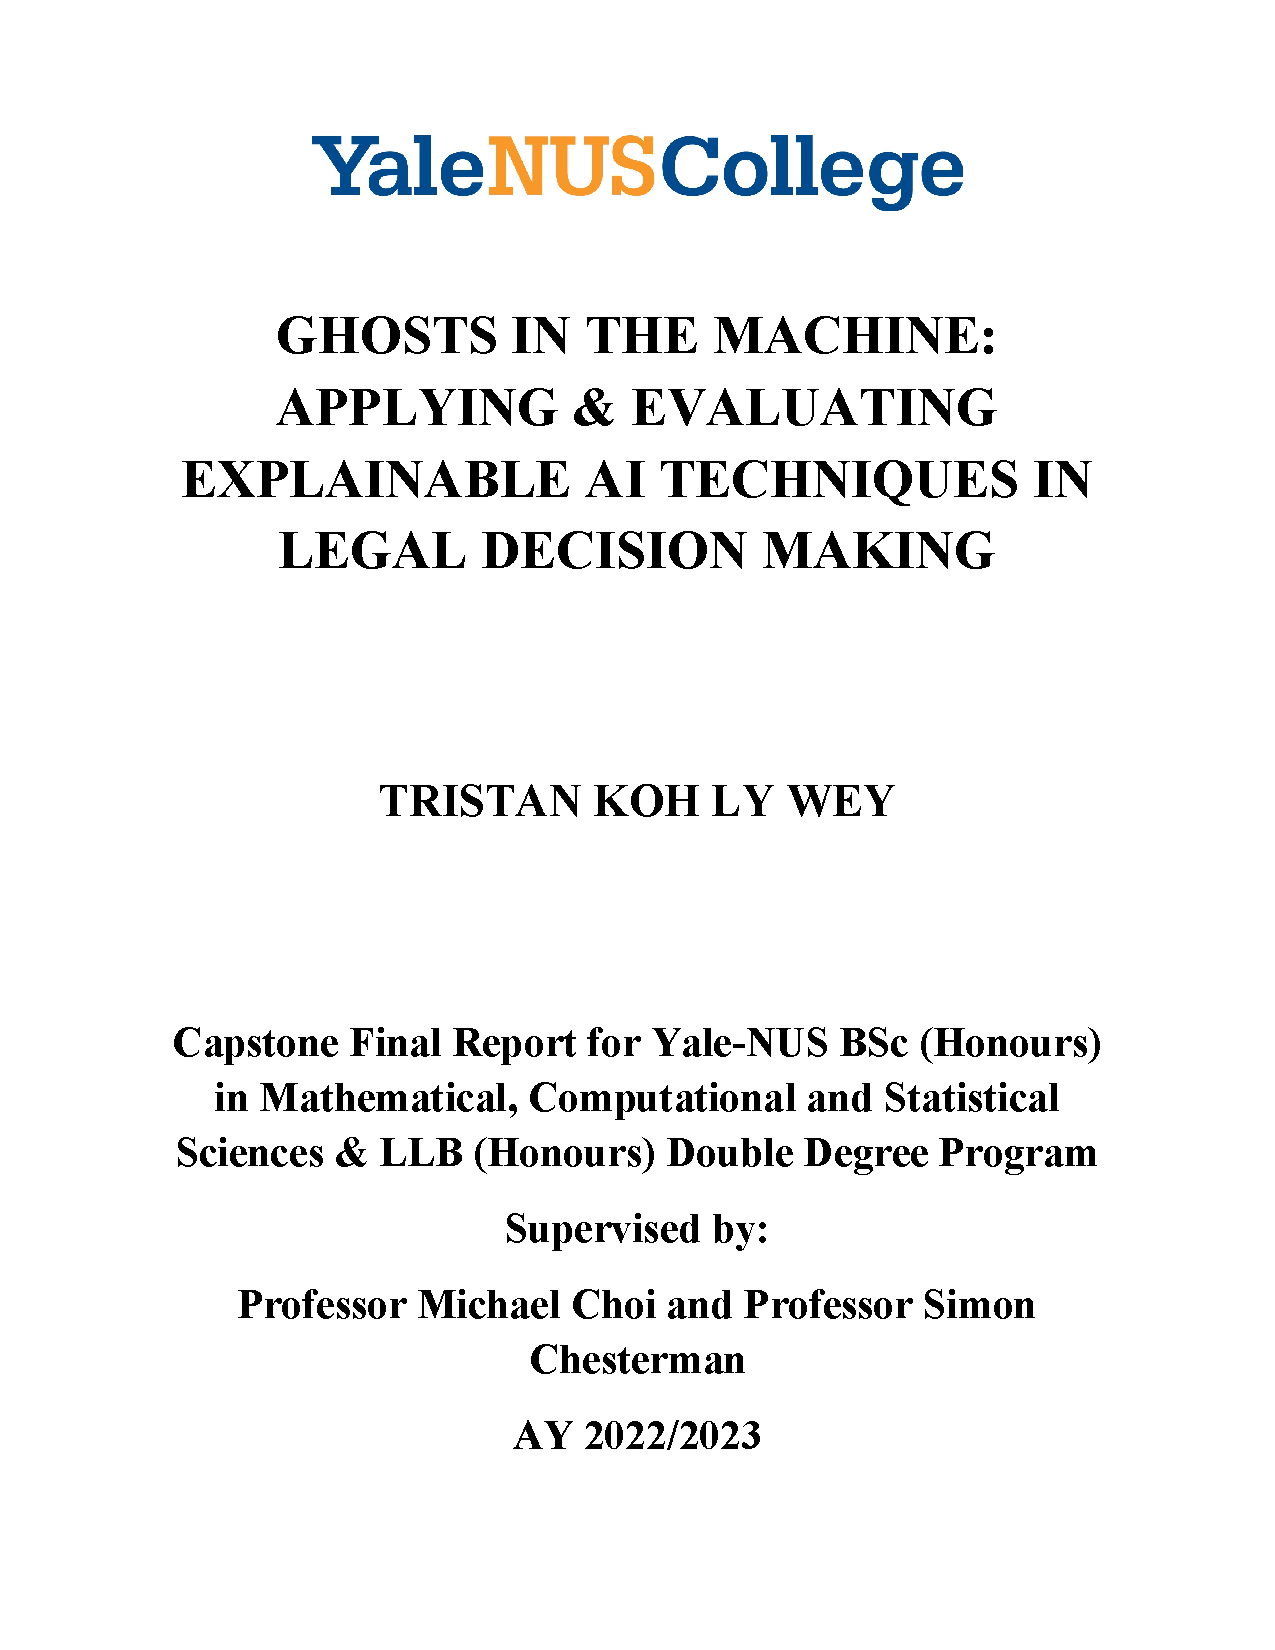
\includepdf[pages=-,pagecommand={},width=\textwidth]{titlepage.pdf}

\end{titlepage}

%----------------------------------------------------------------------------------------
%	DECLARATION & CONSENT
%----------------------------------------------------------------------------------------

% print, sign, and scan the declaration form, then include it here
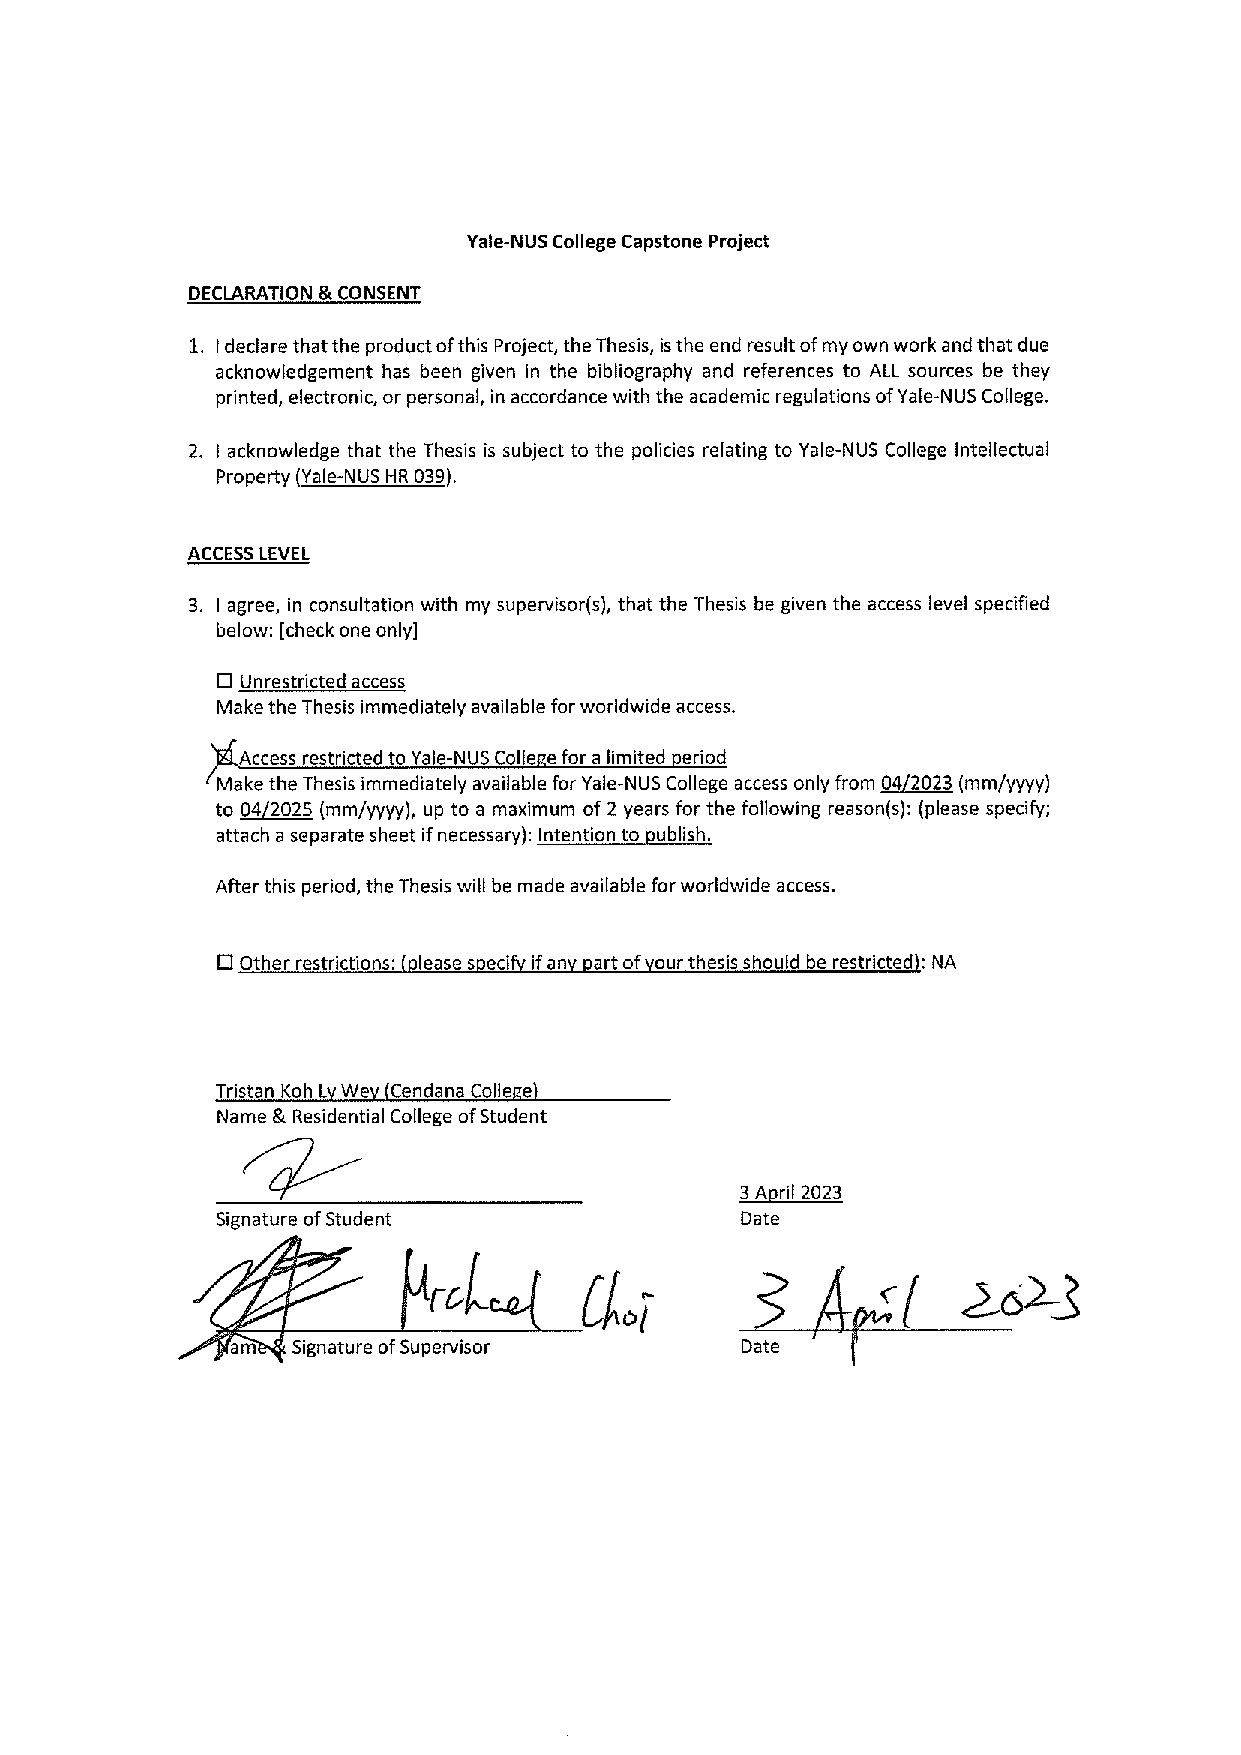
\includepdf[pages=-,pagecommand={},width=\textwidth]{declaration.pdf}

%----------------------------------------------------------------------------------------
%	ACKNOWLEDGEMENTS
%----------------------------------------------------------------------------------------

\begin{acknowledgements}
\addchaptertocentry{\acknowledgementname} % Add the acknowledgements to the table of contents
This capstone would not be possible if not for the gracious provision of the following individuals and groups, and most of all, God.
\end{acknowledgements}

%----------------------------------------------------------------------------------------
%	ABSTRACT PAGE
%----------------------------------------------------------------------------------------

\begin{abstract}
\addchaptertocentry{\abstractname} % Add the abstract to the table of contents
This capstone assesses the explainability of the visualisations of machine learning models that were trained to identify data practices within apps' data privacy policies. 

In recent years, the performance of machine learning models have increased but have come at the cost of decreased explainability. Machine learning has been gradually adopted in the legal industry to assist with low level legal analysis. This lack of explainability could be a significant hindrance towards greater adoption of artificial intelligence (AI) because the lawyer and law firm that use these models ultimately bear the responsibility of ensuring that their advice is legally accurate.

Separately, data privacy has been subjected to increased regulative oversight. With more ways to collect and use personal data, organisations are more likely to misuse such data. Therefore, users' awareness about how their data is collected and used should be heightened. Similarly, regulators and organisations have increased obligations to ensure that data is being collected and used responsibly.

This capstone uses this data privacy context to train reasonably performing models that are able to detect data practices within apps' data privacy practices. As the predictions of these models could be helpful to users, regulators and organisations, Explainable AI (XAI) techniques are applied on these models to produce visualisations that aim to explain these predictions to these stakeholders that may not be experts in data science. Finally, the effectiveness of these visualisations are assessed by surveying current students and the general public about their self-reported levels of trust, fairness and perceptions of effectiveness of these visualisations.
\end{abstract}


%----------------------------------------------------------------------------------------
% CONTRIBUTIONS
%----------------------------------------------------------------------------------------

% \chapter{Claims}
%
% This paper presents the following original contributions:
%
% \begin{enumerate}
% 	\item A hardware device for haptic sensory substitution along with designs for the construction of such a system.
% 	\item Two implementations of sensory substitution using haptic feedback, continuous and delayed feedback-based spatial navigation tasks, each of which include:
% 		\begin{enumerate}
% 			\item a front-end for providing visual input to the user during the training phase with useful readouts to the researcher,
% 			\item a transmission protocol, which maps information from the task at hand (spatial coordinates, velocity information, etc) to time-based sensor actuation signals (20$^{\circ}$ on servo 1, 35$^{\circ}$ on servo 2, etc) in real-time.
% 		\end{enumerate}
% 	\item An evaluation framework for measuring the performance of a sensory substitution system, which provides sample tasks that can be used to standardise and compare performance across the board for future research.
% 	\item A review of existing hardware and software stacks as well as possible avenues for development based on the developed metrics.
% \end{enumerate}
%
% In addition, code for displaying results in real-time, modules for managing servo overload, network latency and other factors were also written by the author.


% %----------------------------------------------------------------------------------------
% %	DECLARATION PAGE
% %----------------------------------------------------------------------------------------
%
% \begin{declaration}
% \addchaptertocentry{\authorshipname} % Add the declaration to the table of contents
%
% \noindent I, \authorname, hereby declare that this Project, the Capstone Report and associated work listed herein, is the end result of my own work and that due acknowledgement has been given in the bibliography and references to ALL sources printed, electronic, or personal, in accordance with the academic regulations of Yale‐NUS College.
% I acknowledge that the Thesis is subject to the policies relating to Yale‐NUS College Intellectual  Property (Yale‐NUS HR 039).
%
%
% % I confirm that:
% %
% % \begin{itemize}
% % \item This work was done wholly or mainly while in candidature for a research degree at this University.
% % \item Where any part of this thesis has previously been submitted for a degree or any other qualification at this University or any other institution, this has been clearly stated.
% % \item Where I have consulted the published work of others, this is always clearly attributed.
% % \item Where I have quoted from the work of others, the source is always given. With the exception of such quotations, this thesis is entirely my own work.
% % \item I have acknowledged all main sources of help.
% % \item Where the thesis is based on work done by myself jointly with others, I have made clear exactly what was done by others and what I have contributed myself.\\
% % \end{itemize}
%
% \noindent Signed:\\
% \rule[0.5em]{25em}{0.5pt} % This prints a line for the signature
%
% \noindent Date:\\
% \rule[0.5em]{25em}{0.5pt} % This prints a line to write the date
% \end{declaration}
%
% \cleardoublepage

%----------------------------------------------------------------------------------------
%	QUOTATION PAGE
%----------------------------------------------------------------------------------------

\vspace*{0.2\textheight}

\noindent\enquote{\itshape In the doorway of my Father's house I'm Home.}\bigbreak

\hfill Psalm 84 (I'm Home) by Shane and Shane

%----------------------------------------------------------------------------------------
%	LIST OF CONTENTS/FIGURES/TABLES PAGES
%----------------------------------------------------------------------------------------

\tableofcontents % Prints the main table of contents

\listoftables % Prints the list of tables
\label{lst:tabs}

\listoffigures % Prints the list of figures
\label{lst:figs}
%----------------------------------------------------------------------------------------
%	ABBREVIATIONS
%----------------------------------------------------------------------------------------

% \begin{abbreviations}{ll} % Include a list of abbreviations (a table of two columns)
%
% \textbf{LAH} & \textbf{L}ist \textbf{A}bbreviations \textbf{H}ere\\
% \textbf{WSF} & \textbf{W}hat (it) \textbf{S}tands \textbf{F}or\\
%
% \end{abbreviations}

%----------------------------------------------------------------------------------------
%	PHYSICAL CONSTANTS/OTHER DEFINITIONS
%----------------------------------------------------------------------------------------

% \begin{constants}{lr@{${}={}$}l} % The list of physical constants is a three column table
%
% % The \SI{}{} command is provided by the siunitx package, see its documentation for instructions on how to use it
%
% Speed of Light & $c_{0}$ & \SI{2.99792458e8}{\meter\per\second} (exact)\\
% %Constant Name & $Symbol$ & $Constant Value$ with units\\
%
% \end{constants}

%----------------------------------------------------------------------------------------
%	SYMBOLS
%----------------------------------------------------------------------------------------

% \begin{symbols}{lll} % Include a list of Symbols (a three column table)
%
% $a$ & distance & \si{\meter} \\
% $P$ & power & \si{\watt} (\si{\joule\per\second}) \\
% %Symbol & Name & Unit \\
%
% \addlinespace % Gap to separate the Roman symbols from the Greek
%
% $\omega$ & angular frequency & \si{\radian} \\
%
% \end{symbols}

%----------------------------------------------------------------------------------------
%	DEDICATION
%----------------------------------------------------------------------------------------

% \dedicatory{}

%----------------------------------------------------------------------------------------
%	THESIS CONTENT - CHAPTERS
%----------------------------------------------------------------------------------------

\mainmatter % Begin numeric (1,2,3...) page numbering

\pagestyle{thesis} % Return the page headers back to the "thesis" style

% Include the chapters of the thesis as separate files from the Chapters folder
% Uncomment the lines as you write the chapters

% Chapter 1

\chapter{Introduction} % Main chapter title

\label{chapter1} % For referencing the chapter elsewhere, use \ref{Chapter1}

%----------------------------------------------------------------------------------------
\section{Motivation and significance}
A question was posed in 2017: "Will there be a software service for the generation of explanations and arguments in law that will assist in structuring explanations of answers and supportive legal arguments?" (\cite{ashley_2017}). This question seems close to getting an answer in 2023 with the release of ChatGPT (\cite{openai}) to the general public. Consider the following conversation with ChatGPT where I documented some of its legal writing abilities\footnote{The question prompts and the names of the specific writing techniques were adapted from \cite{bishop2023computer}.}: 
\begin{enumerate}
  \item Explaining technical concepts. 
  \begin{itemize}
    \item[Q:] Explain what the eggshell skull rule means in negligence law. 
    \item[A:] The "eggshell skull" rule is a principle in tort law that states that a defendant is liable for all damages suffered by a plaintiff, even if the plaintiff's injuries are unusually severe or unexpected. The rule means that the defendant must take the plaintiff as they find them, meaning that they cannot argue that the plaintiff's injuries would not have been so severe if they were a "normal" person.
  \end{itemize}
  \item Adjusting for level and tone. 
  \begin{itemize}
    \item[Q:] Explain the eggshell skull rule like I'm five.
    \item[A:] The "eggshell skull" rule means that if someone hurts another person, they are responsible for all the harm they cause, even if the person they hurt is more easily hurt than most people. It's like if you accidentally hit someone on the head and they have a very fragile skull, you would be responsible for all the damage, even if it's worse than if you hit someone with a normal skull. So you have to be extra careful not to hurt someone, even if they seem more delicate or breakable than most people.
  \end{itemize}
  \item Providing a legal opinion. 
  \begin{itemize}
    \item[Q:] I think that the eggshell skull rule is unfair. Can you make that sound academic?
    \item[A:] Certainly. One could argue that the eggshell skull rule is inequitable, as it places an undue burden on defendants to anticipate and accommodate a plaintiff's pre-existing condition or vulnerability. By imposing liability on defendants for the full extent of the harm caused, regardless of the extent to which the harm would have been suffered by a normal person, the rule ignores the fact that the plaintiff's fragile condition is not the fault of the defendant. Additionally, the rule may incentivize plaintiffs to conceal pre-existing conditions, thereby undermining the efficiency of the tort system.
  \end{itemize} 
\end{enumerate}

In 2017, some commentators opined that AI would be unlikely to take over higher-value roles of the lawyer such as advising clients, writing legal briefs, negotiating and appearing in court (\cite{legaltech_nytimes}). However, as seen from the above, ChatGPT seems to have the ability to automate (or at least assist) these areas of legal practice, except perhaps negotiation and court appearances since ChatGPT does not have a physical presence. Indeed, most recently, ChatGPT has been said to have "the markings of an advocate" (\cite{legaltech_reuters}).

ChatGPT is the most recent AI model that uses advanced natural language processing (NLP). Natural language forms the bread and butter of the legal industry, as it is expressed in contracts, judgements and legislation. The legal industry has been adopting more machine learning tools to automate and assist low level legal analysis. Worldwide legal tech market revenues were at 27.6 billion USD and is projected to to grow at a compound annual growth rate of 4\% to 35.6 billion USD by 2027 (\cite{statista}). As early as 2018, LawGeex, a contract review startup, compared the performance of lawyers vs LawGeex's machine learning model in reviewing standard template Non-Disclosure Agreements (NDA). The model beat the humans both in terms of accuracy and time, with the model having a 94\% accuracy rate and taking 26 seconds to complete the review. In comparison, the lawyers had an average accuracy of 85\% and took 92 minutes to finish the task (\cite{lawgeex}). More significantly, at the end of 2022, OpenAI's AI model GPT (Generative Pre-trained Transformer)\footnote{The GPT is also used for ChatGPT.} took the US bar examination and got 50\% of the questions correct, and performed at a passing rate for both Evidence and Torts (\cite{bommarito2022}).

Like the models that were trained by LawGeex and OpenAI, most legal tech tools that conduct low level legal analysis use natural language processing (NLP) techniques. NLP is a branch of AI that gives computers the ability to understand text and spoken words as how human beings would understand (\cite{ibm_nlp}). While NLP techniques have substantially increased in performance in recent years, it has come at the cost of the explainability of their predictions because of models that are architecturally more complex (\cite{zini2022}). This issue of explainability is exemplified by the last question I posed to ChatGPT about its view on the egg-shell skull rule:

\begin{itemize}
  \item[Q:] How did you think of that answer?
  \item[A:] As an AI language model, I was programmed to provide responses based on a given prompt. In this case, I generated a response to your prompt based on my training data and my understanding of the English language.
\end{itemize}

ChatGPT does not seem to be able to explain its views like how a typical human would\footnote{Further prompting led ChatGPT to provide a list of academic papers that support its view.}. This lack of explainability could potentially be a significant hindrance towards NLP's further adoption within the legal industry because the lawyer and the law firm which use these models still ultimately bear the legal responsibility of ensuring that the analysis is legally sound. For example, r5(2)(c) of the Legal Profession (Professional Conduct) Rules 2015 states that a legal practitioner must act with reasonable diligence and competence in the provision of services to the client. A lawyer that relies on the analysis of legal tech tools and does not understand how the analysis was produced could be considered as lacking in diligence and competence.

Nevertheless, the intersection in skillset between data science and legal analysis is still nascent and it is unrealistic to expect all legally trained personnel to be trained in data science to the extent required to interpret the predictions of machine learning models without aid. At the same time, explainable AI (XAI) techniques and research have been rising in popularity since 2020 (\cite{linardatos2020}) but have not been specifically applied onto legal text. Therefore, this capstone aims to bridge the gap between the lawyer and the data scientist by using XAI techniques to explain the predictions of machine learning models. 

Separately, the widespread collection and use of data by organisations in recent years has led to an increase of regulations governing data privacy. This "datafication" of society includes the "transformation of interactions into data that can be valued and used for predictive analysis". Governments have therefore stepped up their efforts to guarantee privacy, with 145 countries having enacted data protection legislation in 2021 (\cite{gstrein2022}). With more sophisticated regulation comes increased difficulties for organisations to ensure that they are complying with these regulations, and for governments to enforce them. A possible area of legal tech would be tools to aid in the compliance of these regulations. Therefore, I focus on NLP and XAI in the specific context of data privacy. This context provides a realistic evaluation of the interpretability of models that are trained on legal texts relating to data privacy\footnote{All code and analysis used in this capstone can be found at \url{https://github.com/TristanKoh/capstone-repo/}.}.

\subsection{The increasing opacity of NLP and the rise of XAI}
\label{chap1:increasing_opacity}
In NLP, there are inherent difficulties in translating natural language to a mathematical representation that can be understood by the computer. Consider the sentence: "I am cow." Using a Bag-of-Words approach which represents words in terms of their frequency in the sentence, the word "cat" can be represented as:

\begin{lstlisting}
  cow = [0, 0, 1]
\end{lstlisting}

Therefore every word in this sentence can be encoded as: 

\begin{lstlisting}
  I = [1, 0, 0]
  am = [0, 1, 0]
  cow = [0, 0, 1]
\end{lstlisting}

Each word can then be represented as a point with $x, y, z$ coordinates in a three-dimensional space. The plane that passes through all three points would be a graphical representation of the sentence "I am cow". Mathematically, the equation $x + y + z - 1 = 0$ describes the sentence. Clearly there is a big difference in abstraction between the original sentence and the mathematical representation of the same sentence! Without knowing the process of how this equation was derived from the sentence, this equation could possibly refer to any other 3D object, such as the surface of a table.

Further, the Bag-of-Words approach only represents the sentence by the number of occurrences of each word in the sentence. The semantic difference between "I am cat" and "I am cow" (both are four legged animals that are mammals) vs "I am book" and "I am cow" (a cow is a living thing while a book is non-living) is not captured at all by the Bag-of-Words representation\footnote{Furthermore, these two sentences cannot be represented graphically since it introduces a fourth dimension.}. To the computer, "I am cat" and "I am book" are equally different from "I am cow" since both sentences respectively contain an instance of "cat" and "book" which "I am cow" does not contain. In fact, the sentence "I am cow cow" would make sense to the computer even though it makes no sense semantically.

Evidently, even the simplest word representation in NLP poses significant limitations in capturing how humans understand language. Word representations have since progressed tremendously in capturing more semantic meaning, as exemplified by GPT being able to pass certain subjects in the US bar exam. However, to capture such semantic meaning requires more abstraction and further increases the opacity and decreases the interpretability of NLP models. Hence, there is an inverse relationship between performance / opacity and interpretability.  This is typically described as the "black-box" problem of AI: only the inputs and outputs to the system can be observed, but how the model derived the outputs from the inputs is not known (or at least not easily understood) because it is difficult to know exactly how the model is programmed (\cite{zednik2021}).

Therefore, XAI for NLP has been designed to combat such issues. Explainability in this context is seen "from the perspective of an end user whose goal is to understand how a model arrives at its result" (\cite{danilevsky2020}). XAI aims to reduce the abstraction and opacity of NLP techniques so that end users can understand how the model arrived at a decision, which makes the "black-box" more of a "glass-box". However, there is not much consensus about what "explainable" means. While the general agreed upon goal of XAI is to "completely, accurately and clearly quantify the [model's] logic", there is no consistent use of the terms "explainability, interpretability and transparency". Interpretability is sometimes used to describe the model's internal logic and explainability as the ability of the user to understand that logic. In other cases, explainability is the attempt to explain the model's logic post-hoc without necessarily being representative of the model's true decision (\cite{rosenfeld2021}). Since arguing what should be the "correct" definition of explainability is out of the scope of this capstone, I use explainability and interpretability to refer to the general goal of XAI as stated above.

Another growing area of discourse is differentiating what explainability means to different users of the model who have different objectives for the explanations. For example, what could be explainable to data scientists may not be explainable to laypersons. While data scientists may find that providing more technical details about the model would make the model more explainable, laypersons might be more confused if too many details are provided. Further, if a person wants the model to explain why it recommended a certain product over another to purchase on Amazon, the type and level of detail of explanation would be very different compared to a situation where the model predicts that the accused has a higher risk of recidivism which therefore warrants a longer prison term (\cite{rosenfeld2021}). Therefore, assessing the effectiveness of XAI is highly dependent on the specific context and needs of the users. As will be explained in the following section, I focus specifically on what explainability means to three different stakeholders, the consumer, organisation and state for the purposes of analysing apps' data privacy policies.

\subsection{The importance of XAI in data privacy regulation}
As with any regulatory activity, there are three stakeholders: The consumer, the organisation and the state. The importance of XAI in data privacy can also be analysed from the perspectives of these three stakeholders.

\subsubsection{The consumer}
It is uncontroversial that data privacy policies on websites and software are rarely read, and even if they are read, consumers are unlikely to fully understand them because of the use of extensive legalese. Using NLP, Wagner conducted a text analysis of privacy policies from 1996 - 2021, and made the following findings (\cite{wagner2022privacy}): 

\begin{enumerate}
  \item The length of the average policy has doubled in the last 10 years, with the introduction of the General Data Protection Regulation (GDPR) and the California Consumer Privacy Act (CCPA) leading to significant increases in length.
  \item In 2021, the average Flesch Reading Ease of the policies is roughly the same as compared to academic articles such as the Harvard Law Review.
  \item In 2021, the average policy takes 17 minutes to read, and the annual reading time per consumer is more than 400 hours which is more than an hour per day\footnote{Assuming that a consumer visits 1462 unique websites each year.}.
  \item Policies have including more vague wording and invasive data privacy practices, such as implicit collection of location data, no specification as to whether data is anonymised, no meaningful choice given to consumers when there is a change of policy, and generic wording about security measures used to protect data.
\end{enumerate}

The increasing unreadability of data privacy policies poses a significant challenge to the effectiveness of data privacy regulation given that the current model of regulation depends on the consumer giving consent that is informed and freely given (\cite{mantelero_2014})\footnote{Mantelero also discusses a different model of data regulation to combat the issues of the current informed consent paradigm, but that is out of the scope for this capstone.}. Combined with the datafication of society, consumers have diminishing control over how their data is collected and used. 

In view of the unreadability of data privacy policies, legal tech that leverages on XAI can be useful to reduce this unreadability. Legal tech able to analyse and explain the implications of data privacy policies in simple terms to the consumer would greatly aid making these policies more accessible to the consumer, help in allowing them to make informed consent, and saves them time and money as compared to seeking legal advice.

\subsubsection{The organisation}
Though there are many data privacy regulations globally, I focus my analysis on the EU and Singapore since EU's GDPR has the widest scope of any data privacy regulation. I also chose Singapore as this author is based in Singapore. The GDPR is applicable to any personal data processing linked to the EU, either when the entity processing the personal data is established within the EU or when an entity outside the EU offers goods and services to people within the EU (\cite{gdpr_art3}). Therefore, the GDPR is not limited to EU's geographic boundaries and can potentially apply to any entity in any country. Organisations in the EU are subjected to a data subject's "right to explanation". Under Recital 71, data subjects have the right to obtain an explanation of a decision reached solely through automated processing (\cite{gdpr_recital71}). This right could be said to be supported by Art. 22, where data subjects have the right not to be subject to a decision based solely on automated processing (\cite{gdpr_art22}). For example, a bank could use AI to predict the probability of a customer defaulting on a loan. This prediction could be used to justify a decision to deny a loan to the customer. Under the GDPR, the customer has the right to not be subjected to such automated processing and obtain an explanation as to why the model made such a prediction.

In Singapore, explanability of AI decision is found in the non-binding Model AI Governance Framework released by the Personal Data Protection Commission (PDPC) (\cite{ai_modelframework}). While this framework is not specifically about data privacy, AI governance is closely related to data protection as the development of AI models is dependent on how personal data is governed. As part of guidance on the operations management of AI models, organisations are advised to provide explanations on how AI models are incorporated into the decision making process of the organisations so as to build understanding and trust with those stakeholders that use their products. Explainability also forms part of stakeholder communication. In terms of communications with their stakeholders, organisations are advised to develop policies on the type of explanations and when to provide them. Such communication could include explanations as to how the AI model was used in a specific decision. In this regard, the Governance Framework also encompasses the GDPR's right to explanation.

Though there has been debate as to the scope of the GDPR's right to explanation, whether it is binding, and how it is balanced against other interests protected by the GDPR (\cite{chesterman2021_transparency}), such legislation in addition to Singapore's AI Governance Framework that create guidance with regard to the explanability of automated decision making supports the need for further development of XAI specifically in the context of data privacy. The models in this capstone can support the adoption of AI in organisations by providing explanations so as to aid the organisations in checking whether their privacy policies are in compliance with data privacy regulations.

\subsubsection{The state}
At a more macro level, the state's concern when AI is used in legal decision making is maintaining the integrity of the judicial system and regulatory activities. Three challenges arise because of opacity when AI is used in legal decision making in a data privacy context (\cite{chesterman2021_opacity}): 

\begin{enumerate}
  \item Inferior decision making as opacity reduces opportunities to identify wrongdoing or areas of reasoning which can be improved. 
  
  For example, TikTok's algorithm that recommends users' videos on their feed collects and aggregates user data to predict their interests. This algorithm is known to be much more aggressive compared to other social networks and has played a crucial role in its recent spike in popularity (\cite{tiktok_guardian}). It optimises for time spent viewing each video (including the time that the user returns to the same video) to recommend more videos that aim to keep the user scrolling on the app. While TikTok has disclosed the broad factors that the algorithm uses, the actual algorithm is much more nuanced as seen at how an internal company document describes recommending more "sad" content to increase watch time which could lead to videos involving self-harm (\cite{tiktok_nytimes}). With opacity in the algorithm, users (and regulators) do not know how their personal data is being used to recommend them videos. This could lead to adverse social consequences when the algorithm recommends controversial content such as religiously or politically partisan posts. Opacity also prevents regulators from pre-empting or intervening in such undesirable social consequences such as mandating that such recommendation algorithms must have limits to the type of content that can be recommended.
  
  \item Impermissible decisions such as reifying discrimination as opacity masks such decisions with the "objective" nature of AI predictions.
  
  A common example of this is using AI to predict which bank customers would default on their loans. AI models are trained to predict the risk of default based on demographic metrics, such as employment status and income level. If the model assesses the customer is likely to default, the bank would probably not allow the customer to take out a loan. In some jurisdictions, anti-discrimination legislation prevents banks from making such assessments with regard to race, gender, colour, religion etc. which are considered personal data under data privacy regulation\footnote{Such as the Fair Housing Act in the US that makes it unlawful for any lender to discriminate against any person because of race, colour, religion, national origin, sex, handicap or familial status (\cite{fairhousingact}).}. If opaque AI models are used, it would not be possible to ascertain whether these protected personal data are actually used for the prediction. It could be possible to justify a decision not to grant a loan just because the model made a prediction that the customer is likely to default. This prediction could be seen as "objective" as it was made by an algorithm rather than a human even though it actually perpetuates racism because it used race as a predictor (for example). Hence, opacity in AI models potentially pose societal and regulatory issues.

  \item Legitimacy of decisions since the legal system depends as much on the justification of decisions as it does on the decisions themselves.
  
  In the context of data privacy regulation in Singapore, Parliament enacts the PDPA while the PDPC is empowered to create regulations and enforce the PDPA\footnote{Per s65(1) of the PDPA.}. There is an appeal process for cases appearing before the PDPC and the higher courts can overturn the PDPC's decisions\footnote{Per s48Q, s48R and s54 of the PDPA.}. However, when overturning the PDPC's decisions, the higher courts do not disagree with the outcome but they disagree with the reasoning of the PDPC's decision. Assuming that AI models are sophisticated enough to write court judgements, if there was no explanation of the model's judgement, there would be no basis for the higher courts to overturn judgements made by lower courts. 
  
  Further, in common law systems, judges' decisions become part of case law and past decisions become binding on new cases with the same facts (i.e. the doctrine of \textit{stare decisis}). One of the benefits of case law is that it can be developed incrementally and adapted to suit real facts unlike legislation, so that the law actually meets the needs of the parties. While \textit{stare decisis} does not apply to PDPC cases at first instance, the same principle of incrementally developing and applying the law still applies. For example, the quantum of fine imposed on organisations in breach of the PDPA is determined according to how severe the breach is in comparison with similar past cases\footnote{An example would be \textit{RedMart Limited} [2022] SGPDPC 8 at [33].}. If opaque AI is used to write or aid in the writing of these decisions, there would be fewer opportunities to improve the law since the reasoning would likely to be insufficiently explicit. Hence the development of the law would also be impeded.
\end{enumerate}

Hence, the importance of XAI applies across all three stakeholders in data privacy. Consumers can benefit from XAI by making privacy policies more readable. Organisations can use XAI to be more accountable to consumers and regulators by providing explanations for automated decisions. XAI also provides the state with more transparency in regulating organisations' use of AI and aiding in judicial decision making.

\section{Problem statement}
The foregoing analysis of the issues in data privacy and the opacity of NLP models can be summarised as follows: NLP techniques are now much more advanced and can potentially automate some areas of substantive legal reasoning and writing, but has come at the cost of increased opacity of the models. More research has been put into XAI in an effort to combat this opacity, but it is an open question as to whether the explanations are effective to the different users and use cases of the models. Data privacy regulation can benefit from the use of more XAI in automated decision making. Thus, there is a gap in research where XAI is assessed and applied in data privacy. 

Hence, I choose to train AI models that are able to identify data privacy practices in apps' data privacy policies. A privacy practice describes a certain behaviour of an app that can have privacy implications\footnote{This will be further elaborated on when \hyperref[app350_corpus]{the dataset} is introduced.}. In this regard, these models function similarly to that of LawGeex's contract review models which are able to identify the type of clause, such as which party owns the intellectual property arising from the performance of the contract\footnote{Automated contract review models are also able to analyse the level of legal risk associated with any amendments made to the clause, such as if the counterparty amended the wording of the clause to state that only the counterparty owns the intellectual property instead of both contracting parties.}. XAI methods are then used to visualise why the models made such predictions. Such a legal tech tool saves consumers time by highlighting specific data privacy practices upfront so that they can make informed consent. 

I focus on these specific problems for the rest of the capstone:

\begin{enumerate}
  \item Which AI models perform the best on this dataset in terms of precision / recall / F1?
  \item Which models are the most explainable to an audience that includes laypersons and people with domain knowledge in data science and the law, and why?
  \item How would people rate the explainability of a selected XAI technique?
  \item Are there differences in how people rate explainability if they were asked to consider the predictions of these models from the perspective of a consumer, an organisation or the PDPC (as the regulatory authority for data privacy), and why?
\end{enumerate}

\section{Main findings and roadmap}
Chapter~\ref{chapter2} is a literature review of XAI methods of NLP and methods of assessing these XAI methods which forms the justification of the methodology and dataset used. Chapter~\ref{chapter3} presents an exploratory data analysis of the dataset. Chapter~\ref{chapter4} reports the performance of the models that were trained on the dataset. 
%TC:group tabular 0 1
\chapter{Literature review and methodology} % Main chapter title
\label{chapter2} % For referencing the chapter elsewhere, use \ref{Chapter1}

% Define some commands to keep the formatting separated from the content
\newcommand{\keyword}[1]{\textbf{#1}}
\newcommand{\tabhead}[1]{\textbf{#1}}
\newcommand{\code}[1]{\texttt{#1}}
\newcommand{\file}[1]{\texttt{\bfseries#1}}
\newcommand{\option}[1]{\texttt{\itshape#1}}

%----------------------------------------------------------------------------------------

There are four major components to this capstone: The dataset, model training, application of XAI techniques to the trained models and evaluating the effectiveness of these XAI techniques. I provide a literature review and describe the chosen methodology of these components below.

%----------------------------------------------------------------------------------------
%	SECTION 1
%----------------------------------------------------------------------------------------
\section{Dataset: The APP-350 Corpus}
\label{app350_corpus}
The APP-350 Corpus consists of 350 annotated Android app privacy policies. Each data practice ("practice") consists of a data type and a modality. A data type describes a certain behaviour of an app that can have privacy implications (e.g. collection of a phone's device identifier or sharing of its location with ad networks). There are two modalities: \texttt{PERFORMED} (i.e. a practice is explicitly described as being performed) and \texttt{NOT\_PERFORMED} (i.e. a practice is explicitly described as not being performed). Altogether, 57 different practices were annotated. As not all practices had sufficient numbers to train models of sufficient baseline performance, I focused on training models on the top 5 practices by frequency\footnote{The performance of the models of the top $n$ frequently occurring practices is later elaborated on in Chapter~\ref{chapter4}.}. The data types and modalities that are used for the rest of the capstone are provided in Table~\ref{tab:data_practices} and ~\ref{tab:modalities}.

\begin{table}[]
	\resizebox{\textwidth}{!}{%
	\begin{tabular}{|l|p{0.8\linewidth}|}
	\hline
	\textbf{Data Type}                 & \textbf{Description}                                                                                    \\ \hline
	Contact\_E\_Mail\_Address & Describes collection of the user's e-mail.                                          \\ \hline
	Identifier\_Cookie\_or\_similar\_Tech & Describes collection of the user's HTTP cookies, flash cookies, pixel tags, or similar identifiers. \\ \hline
	Identifier\_IP\_Address   & Describes collection of the user's IP address.                                      \\ \hline
	Location                  & Describes collection of the user's unspecified location data.                       \\ \hline
	\end{tabular}%
	}
	\caption{List of top 4 data types and their descriptions.}
	\label{tab:data_practices}
\end{table}

\begin{table}[]
	\resizebox{\textwidth}{!}{%
	\begin{tabular}{|l|p{0.8\linewidth}|}
	\hline
	\textbf{Party}                 & \textbf{Description}                                                                                    \\ \hline
	1stParty & Describes collection of data from the user by the app publisher.                                          \\ \hline
	3rdParty & Describes collection of data from the user by ad networks, analytics services, or other third parties. \\ \hline
	\end{tabular}%
	}
	\caption{List of modalities.}
	\label{tab:modalities}
\end{table}

The APP-350 Corpus was annotated and used in a broader project to train machine learning models to conduct a privacy census of 1,035,853 Android apps \cite{zimmeck2019}. The authors downloaded the data privacy policies of apps from the Play Store with more than 350 million installs (which totalled 247 apps) and 103 randomly selected apps with 5 million installs. In total, there were data privacy policies of 350 apps. All 350 policies were annotated by one of the authors, a lawyer with experience in data privacy law. To ensure reliability of annotations, 2 other law students were hired to double annotate 10\% of the corpus. With a mean of Krippendorff's $\alpha = 0.78$\footnote{Krippendorff's $\alpha$ is a measure of agreement, with $\alpha > 0.8$ indicating good agreement, $0.67 <= \alpha <= 0.8$ indicating fair agreement, and $\alpha < 0.67$ indicating doubtful agreement.}, the agreement between the annotations exceeded previous similar research.

Since the focus of this capstone is to assess XAI methods within a data privacy context, the APP-350 corpus was chosen as it contains real-world data privacy practices from the PlayStore apps. Training models and evaluating XAI techniques on this dataset would provide a realistic indication of their performance. APP-350 is also a labelled dataset, allowing supervised training which provides a better validation of model performance. 

The annotated privacy policies were originally in \texttt{.yml}, with one \texttt{.yml} file containing one app data privacy policy. Each data privacy policy is labelled at both the sentence and segment\footnote{A segment is similar to a paragraph.} level, but to limit the scope of this capstone I focus only on sentence level. The data was restructured from \texttt{.yml} to \texttt{.csv}.

\section{Text representations and models}
\label{sec:classifiers}
\subsection{Literature review}
In NLP, there are two components of a text classifier: The text representation, and the model. In this capstone, I distinguish between "model" and "classifier" for clarity. "Model" refers to the machine learning algorithm used to generate predictions, while "classifier" refers to the combination of a text representation and model that classifies a segment of text to a particular category. I make this distinction because part of this capstone's methodology is testing the explainability of the different combinations of models and text representations, of which both components are needed to form a classifier.

Text representations are methods that translate plain text to mathematical representations that can be understood by a computer. The easiest and most intuitive text representation is a purely count-based approach such as Bag-of-Words, where each word is represented by their frequency in the sentence. These can be categorised as sparse vector representations. However, they do not capture the semantic and syntactic differences of words \cite{liu2020word}. More advanced dense vector representations such as GloVe (Global Vectors) are better able to capture these differences. Generally, these dense vector representations are created through unsupervised learning. Neural networks are trained to predict the target word given surrounding words \cite{liu2020word}. However, to capture such semantic meaning requires more abstraction and further increases the opacity and decreases the interpretability of NLP models. Hence, there is an inverse relationship between performance / opacity and interpretability.  This is typically described as the "black-box" problem of AI: only the inputs and outputs to the system can be observed, but how the model derived the outputs from the inputs is not known (or at least not easily understood) because it is difficult to know exactly how the model is programmed \cite{zednik2021}. In generating text representations of the APP-350 corpus, \cite{zimmeck2019} used a union of Tf-IDF vectors and manually crafted features which were Boolean values indicating the presence or absence of frequently occurring keywords that occurred in each data practice.

Another component of a classifier is the model used to generate predictions. These models can be broadly categorised into classical machine learning models such as logistic regression and decision trees, and neural networks such as GPT. However, while neural networks are higher performing, if simpler models are able to produce reasonable performance, these simpler models should be used instead. Much depends on the complexity of the text corpus, and the engineering task that the model are made for. Classical models are much less complex and therefore more explainable than neural networks, and require much less data to train. For the APP-350 corpus, \cite{zimmeck2019} used support vector machines for classification (SVCs) to achieve reasonable performance. Individual models were then trained for every data practice. For all the classifications (except for four categories), they trained SVCs with a linear kernel and five-fold cross validation. For the four policy classifications, word-based rule classifiers were used instead because of the limited number of training data.

For the top 5 data practices that this capstone is concerned about, \cite{zimmeck2019} were able to achieve F1 scores ranging from 77\% (Identifier Cookie 1st Party), 91\% (Contact Email Address 1st Party) to around 90\% for location related data practices\footnote{Not all the data practices were used in training ($n = 188$) and testing ($n = 100$) these classifiers, so there is no reference performance for some of the data practices that are used in this capstone.}.

\subsection{Methodology}
Given that the focus is on explainability, and in any case the APP-350 corpus is probably too limited to train neural networks\footnote{For example, BERT was trained on the whole Wikipedia (and more), while GPT-2, the second iteration of GPT, was trained on 45 terabytes of data.}, I focus only on training classical models in this capstone. Since sparse vector representations and classical models have performed well for the APP-350 corpus as seen above, I use SVCs and Tf-IDF. For the sake of comparison, I also use logistic regression and pre-trained GloVe embeddings.

The idea behind Tf-IDF is that words that are frequent in a document but rare across the rest of the corpus are more important in distinguishing the document from others. The Tf-IDF metric for a word in a document is calculated by multiplying two different metrics:

\begin{enumerate}
	\item Term frequency (TF) of a word in a document. This is the number of times the word appears in a document.
	\item Inverse document frequency (IDF) of the word across a set of documents. This is calculated by taking the total number of documents and dividing it by the number of documents that contain the specific word. This calculates the rarity of the term across all the documents. The closer the IDF of a word is to 0, the more common the word is.
\end{enumerate}

In comparison, GloVe as a dense vector representation is able to better model semantic differences mathematically in the following way: $\text{King} - \text{Man} + \text{Woman} = \text{Queen}$ \cite{vector_differences_2015}. GloVe is an unsupervised learning algorithm for obtaining vector representations for words. The length-50 vectors used in this capstone are pre-trained using this algorithm on Wikipedia and news articles \cite{pennington2014glove}. The main idea behind GloVe is to learn text representations by considering the statistics of words that occur together in a corpus. These statistics capture how frequently different pairs of words occur together in the text. GloVe builds a matrix from these statistics, where each element represents the number of times two words appear together in the same context. The matrix is then factorized into a product of two low-rank matrices, where each row in one of the matrices represents a vector representation of a word. This results in dense, fixed-size vector representations for each word in the corpus that encode their meaning and relationships with other words in the corpus.

In terms of tokenisation, for both Tf-IDF and GloVe representations, text was lowercased and stop words were removed. No stemming and lemming was conducted. For Tf-IDF specifically, 1-gram to 4-grams were generated. For GloVe, length 50 pre-trained vectors were used to tokenise individual words, and then averaged across all of the words to represent one document.

In terms of models for prediction, I use SVC with a linear kernel. SVC works by finding the a linear hyperplane in a high-dimensional space that separates the different classes of data points with the maximum margin of separation (Figure~\ref{fig:svc_viz}). The hyperplane functions as a decision boundary and the margin is the distance between the hyperplane and the nearest datapoints from each class. I also use scikitlearn's SGDClassifier that implements linear SVC using gradient descent, which is another optimisation method apart from a linear kernel. Logistic regression is used as a baseline classifier for its simplicity. Logistic regression predicts the probability of a multi-class target variable as a function of the input features. The sigmoid function is usually used to transform the linear combination of features into a probability value between 0 and 1 (Figure~\ref{fig:log_reg_viz}). While I also trained ensemble classifiers (AdaBoost, GradientBoost, Random Forest), the performance of these models were roughly the same or less than logistic regression and SVC. Hence, I excluded them from further analysis.

\begin{figure}[!ht]
	\centering
	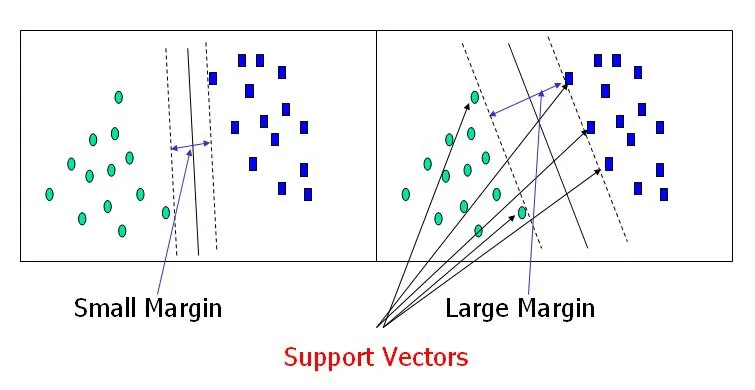
\includegraphics[width=1\linewidth]{figures/svc_viz.png}
	\caption{Finding the hyperplane in SVC \cite{svc_viz}.}   
    \label{fig:svc_viz}
\end{figure}

\begin{figure}[!ht]
	\centering
	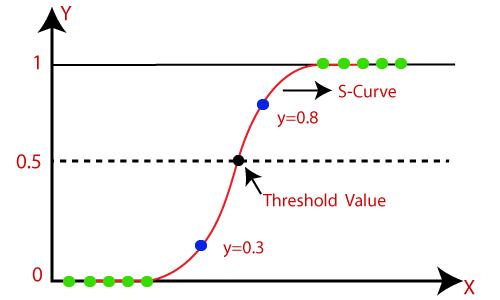
\includegraphics[width=1\linewidth]{figures/logistic_reg.png}
	\caption{Sigmoid function in logistic regression \cite{log_reg_viz}.}   
    \label{fig:log_reg_viz}
\end{figure}


%-----------------------------------
%	SECTION 2
%-----------------------------------
\section{XAI methods for NLP}
\subsection{Literature review}
XAI for NLP have two broad characteristics: Local vs global, and self-explaining vs post-hoc. Thus, there are four possible categories of XAI as seen in Table~\ref{tab:xai_methods}.

\begin{table}[!ht]
	\resizebox{\textwidth}{!}{
	\begin{tabular}{|l|p{0.8\linewidth}|}
	\hline
	\textbf{Category}      & \textbf{Description}                                                                                                                            \\ \hline
	Local Post-Hoc         & Explain a single prediction by performing additional operations (after the model has made a prediction)                                         \\ \hline
	Local Self-Explaining  & Explain a single prediction using the model itself (calculated from information made available from the model as part of making the prediction) \\ \hline
	Global Post-Hoc        & Perform additional operations to explain the entire model's predictive reasoning                                                                \\ \hline
	Global Self-Explaining & Use the predictive model itself to explain the entire model's predictive reasoning                                                              \\ \hline
	\end{tabular}
	}
	\caption{The four categories of XAI for NLP, adapted from \cite{danilevsky2020}.}
	\label{tab:xai_methods}
	\end{table}

Some classical models such as logistic regression can be considered local and global self-explaining models. The coefficients of the features show the relative importance of each feature towards making the prediction. These coefficients are generated as part of the model training process and make it self-explaining. Logistic regression is also globally explainable since it models a deterministic function (sigmoid function), and this function serves as the "reason" for any prediction by the model. However, neural networks are not self-explaining by nature, in part as they are non-linear and are fitted onto high-dimensional data, in additional to the large numbers of parameters that make it difficult to ascertain the interaction between different features when a prediction is made. Therefore, post-hoc methods of explanability have to be used instead. 

\begin{figure}[!ht]
	\centering
	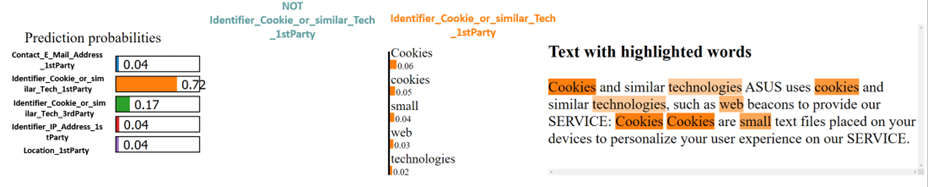
\includegraphics[width=1\linewidth]{figures/explanations_visualisations/section_4a/Picture1.png}
	\caption{Sample visualisation of LIME}   
    \label{fig:lime_sample}
\end{figure}

\subsection{Methodology}
I use LIME (Local Interpretable Model-agonistic Explanations), a local post-hoc XAI method that is also model agnostic \cite{lime}. Given a trained NLP model, LIME generates a set of perturbations on the input sentence by randomly replacing some of the words with similar words. These perturbed samples are passed to the NLP model for prediction. Using these predictions, LIME fits a simple self-explaining model (such as a linear regression or a decision tree) to explain these predictions. Through this local self-explaining model, LIME is able to generate the contribution of each feature to a particular prediction for a single sample. Figure~\ref{fig:lime_sample} is an example of how an explanation of LIME can be visualised. Since LIME is a local, post-hoc method that uses a surrogate model to generate explanations, one disadvantage is that it may not fully represent how the underlying model actually made its prediction. Nevertheless, LIME has been found to be able to generate explanations that are faithful to the underlying model even just by using linear models for the surrogate model \cite{lime}.

I chose to use LIME because it is model agnostic which allows easy experimentation with different combinations of text representations and models. Though logistic regression and SVC may be inherently self-explaining, I apply LIME on them because it visualises the feature importance without needing survey respondents to interpret coefficient scores of these models which can be inaccessible to those without a data science background. I apply LIME on the different combinations of text representations and models and compare the explainability of LIME's explanations. I presented these explanations to the survey respondents without any amendments to the code output, except for minor editing to the labels in the figure because some labels were cut-off.

\section{Evaluating the effectiveness of XAI methods}
\subsection{Literature review}
There is no consensus of the methods or standards of assessing XAI techiques \cite{vilone2021}. Standards of explainability are highly dependent on the purpose of generating the explanations. A few purposes have been suggested \cite{doshi-velez2017}:
\begin{enumerate}
	\item \textit{Global vs local:} A scientist inspecting a model predicting rainfall would require global explanation since he would be concerned with finding a long-term patterns, while a consumer who failed to obtain a loan would only require a local explanation to justify why the model made that specific decision.
	\item \textit{Area and severity of incompleteness of the problem:} A potential buyer of an autonomous vehicle (AV) would want a general overview of how AVs work, while a regulator may have specific explanation requirements such as whether a model detects a pedestrian 10 metres before collision.
	\item \textit{Nature of user expertise:} A layperson with no training in credit worthiness would not expect details of large complicated models in relation to the model's prediction of his credit rating, compared to an auditor that would expect explanations of comparable granularity and nuance as human auditors.
\end{enumerate}

Within the legal context, what could be insufficiently explainable for non-discrimination law \cite{vale2022explainable} might not apply \textit{mutatis mutandis} to the GDPR. Indeed, different standards for explainability have been argued to apply across contract, tort and banking law \cite{hacker2022varieties}. In any case, this capstone makes no claim as to the applicable standard for explainability for data privacy, and merely serves as empirical insight of explainability from the perspectives of the three stakeholders in data privacy.

In terms of methods of assessing XAI, human evaluation has been frequently utilised \cite{danilevsky2020}. This involves asking humans to evaluate the effectiveness of the explanations in various ways (Table~\ref{tab:human_eval_xai}). The metrics being evaluated include fidelity (how much the explanation reflects the actual workings of the model), comprehensibility (how easily understood are the explanations), and others. However, many studies also do not state what is being evaluated. 

\begin{table}[!ht]
	\resizebox{\textwidth}{!}{%
	\begin{tabular}{|p{0.2\linewidth}|p{0.85\linewidth}|}
	\hline
	\textbf{Method}                 & \textbf{Description}                                                                                                                                        \\ \hline
	Binary forced choice            & Humans are presented with pairs of explanation, and must choose the one that they find of higher quality.                                                   \\ \hline
	Forward simulation / prediction & Humans are presented with an explanation and an input, and must correctly simulate the model's output.                                                      \\ \hline
	Counterfactual simulation       & Humans are presented with an explanation, an input, and an output, and are asked what must be changed to change the model's prediction to a desired output. \\ \hline
	\end{tabular}
	}
	\caption{Methods of measuring human evaluation of XAI \cite{doshi-velez2017}.}
	\label{tab:human_eval_xai}
\end{table}

Human evaluation has been conducted within a legal context \cite{gorski2021}. The authors trained a CNN on a dataset that contained 50 decisions issued by the Board of Veterans' Appeals of the US Department of Veterans Affairs. Each sentence was annotated according to a type of legal reasoning (e.g. fact finding, legal reasoning, application of legal rule etc.). The focus of the research was to evaluate different XAI methods and lawyers' perceptions and expectations of XAI. Lawyers were asked to rate different XAI visualisations of the same 6 correctly classified sentences on a scale from 0 (worst) to 10 (best). Further, the lawyers that were surveyed were generally optimistic about the use of AI in law, with most agreeing that the explanations generated should be supplemented by further background knowledge, and that the model should be fair, lack bias, transparent and have awareness of the consequences of the AI-assisted / AI-automated decision. Lawyers also agreed that AI should increase automation and reduce their manual effort. 

In addition, there is no agreed upon definition of "explainability". Explainability could be influenced by other value-laden terms, such as, \textit{inter alia}, trust, effectiveness, fairness, bias, and the consequence of making a wrong prediction \cite{rosenfeld2021}. The relative importance of these values and overall requirement of explainability is necessarily dependent on the purpose and user of the explanation. Values such as fairness, bias, risk and trust could be argued to be of specific importance in a legal context which includes data privacy. The notion of "rule of law" encompasses these values and legal systems are arguably judged according to such values \cite{greenstein2022}. Nevertheless, there is no definitive position as to how these values can be used to evaluate XAI techniques that are specifically used within a legal context.

\subsection{Methodology}
With the foregoing discussion in mind, I expand upon the methodology of \cite{gorski2021} by testing the effectiveness of LIME by varying the different purposes of explanations and methods of evaluation that were identified above. The primary method of evaluating LIME in this capstone is human evaluation through a survey. The survey was designed containing the following parts\footnote{The full survey can be found \href{https://github.com/TristanKoh/capstone-repo/blob/448263a933ae787027298e266f9202e7b3077524/survey/survey_questions.pdf}{here}, and a summary of the responses can be found \href{https://github.com/TristanKoh/capstone-repo/blob/448263a933ae787027298e266f9202e7b3077524/survey/survey_responses.pdf}{here}. Visualisations that were of significance to the analysis are provided later in Chapter~\ref{chapter4}.}:
\begin{enumerate}
	\item \textbf{Part 1: Demographic data and beliefs relating to data privacy and AI.} Respondents were asked to provide their major or subject area expertise if they had graduated, and their level of experience with AI / data science and data privacy / law. This is used as a proxy for their level of expertise in AI or data science. Respondents are also asked to rate how much they think AI is useful, how far AI could be a risk, as well as how far they are concerned about their data privacy. This is used to understand the respondents' beliefs such that their assessment of LIME and the models can be evaluated in the context of these beliefs. Further cross-sectional analysis of the survey data can also be conducted using these data.
	\item \textbf{Part 2: Rating of explainability metrics from the perspectives of three stakeholders in data privacy.} After a brief explanation of the data practices and how NLP works, respondents were provided with three contexts (app developer, PDPC \& user). All three contexts relate to solely relying on the predictions of the classifier to make a decision in relation to a finding of a breach of the PDPA, and are meant to vary the purposes of the explanation according to the three purposes suggested by \cite{doshi-velez2017} above, as well as the legal \& programming expertise of the end-user of the explanation. The consequence of making a wrong decision was kept constant across the contexts by stating that a \$10,000 fine would be imposed as a consequence of a finding that the PDPA was breached.
	
	After reading each context, the respondents were required to rate their beliefs relating to the use of the classifier in that particular context across four metrics: Effectiveness of model, Fairness, Risk to society, and trust in the model. These metrics were chosen as they are values of importance specifically to a legal decision making context. The purpose is to investigate how these values that relate to explainability can vary according to the purposes of the explanation.
	\item \textbf{Part 3: Rating of LIME visualisations of four classifications by the same classifier (Logistic regression + Tf-IDF).} Respondents were asked to rate: (1) how far they understood why the model made the prediction, and (2) how far they found the visualisation easy to interpret. The intent is to evaluate both the underlying XAI technique (LIME) and the visualisation of the technique. For three classifications, respondents were given a counterfactual sentence replaced with words that were considered important by the classifier, and asked to predict whether the sentence would be classified under \texttt{Identifier Cookie 1st Party}. Counterfactual simulation is meant to provide another method to measure explainability, aside from self-reported scores.
	\item \textbf{Part 4 \& Part 5: Choosing the more interpretable visualisation from a pair of identically classified sentences.} This uses binary forced choice to evaluate which text representation and model are more interpretable. Part 4 of the survey presents 3 pairs of visualisations from SVC + GloVe and Logistic regression + GloVe (controlling for text representation) and Part 5 presents another 3 pairs of visualisations from SVC + Tf-IDF and SVC + GloVe (controlling for model). Respondents were not told that the visualisations were produced by different models or text representations. The respondents' choices are then totalled up and compared against performance metrics (P/R/F1) of the classifiers to with these metrics acting as a "ground truth". This is to investigate whether there is a relation between interpretability and model performance.
	\item \textbf{Part 6: Rating of the same explainability metrics for the same three contexts.} Respondents are finally asked to view the same three contexts and answer the same questions in Part 2, and their reported scores in Part 6 are tested for statistical increase / decrease compared to their initial scores in Part 2. This evaluates whether viewing the explanations significantly changed the respondents' beliefs of the use of the classifier in the three contexts according to the four metrics, and whether there are relations and trends between the individual metrics and contexts. Part 2 acts as a control variable in this comparison.
\end{enumerate}

The survey was hosted on Google Forms, and respondents were anonymously recruited through friends and acquaintances of this author. The only restriction on recruitment was an age requirement of 18 and over for NUS / Yale-NUS students, or 21 and over for the general public due to Yale-NUS Ethics requirements. No personal identifying information of the respondents were collected.
% Chapter Template

\chapter{EDA and classifier performance} % Main chapter title

\label{chapter3} % Change X to a consecutive number; for referencing this chapter elsewhere, use \ref{ChapterX}

\section{EDA}
There are a total of 18829 annotated sentences and the top 10 frequently occurring practices make up close to 60\% of all sentences (Figure~\ref{fig:eda_data_practice}). The bottom 10 frequently occurring practices make up approximately 1\% of the dataset. There does not seem to be much variation in sentence length for the top 10 frequently occurring practices, since the standard deviation for the mean is approximately 2.5 words and the median 1.9 words (Table~\ref{tab:summary_top_10_practices}) and as seen by similar interquartile range (IQR) (Figure~\ref{fig:boxplot_top_10}). This could indicate similar sentence complexity across the practices. The mean of the sentence lengths for all top 10 practices are slightly greater than the median, which suggest some outliers with very long sentences (Figure~\ref{fig:graph_sentence_length}) that cause a slightly right skew distribution (Figure~\ref{fig:hist}). The distributions are also unimodal, with the mode around 20.

% \begin{table}[!ht]
% 	\resizebox{\textwidth}{!}{
% 	\begin{tabular}{lrrrr}
% 	\toprule
% 									  practice &  counts &  mean sentence length &  median sentence length &  percentage of total \\
% 	\midrule
% 	Identifier\_Cookie\_1stParty &    2107 &             25.4 &                    22.0 &           11.2\% \\
% 			   Contact\_E\_Mail\_Address\_1stParty &    2106 &             28.7 &                    25.0 &           11.2\% \\
% 							 Location\_1stParty &    1514 &             29.2 &                    24.0 &           8.1\% \\
% 	Identifier\_Cookie\_Tech\_3rdParty &    1250 &             27.3 &                    24.0 &           6.6\% \\
% 				Identifier\_IP\_Address\_1stParty &    1005 &             30.9 &                    27.0 &           5.3\% \\
% 				 Contact\_Phone\_Number\_1stParty &     970 &             29.1 &                    25.0 &           5.2\% \\
% 				 Identifier\_Device\_ID\_1stParty &     697 &             32.4 &                    28.0 &           3.7\% \\
% 			   Contact\_Postal\_Address\_1stParty &     597 &             28.9 &                    26.0 &           3.2\% \\
% 										   SSO &     504 &             32.6 &                    28.0 &           2.7\% \\
% 					  Demographic\_Age\_1stParty &     428 &             33.1 &                    26.0 &           2.3\% \\
% 	\bottomrule
% 	\end{tabular}
% 	}
% 	\caption{Summary statistics per practice of top 10 occurring practices.}
% 	\label{tab:top_10_sentence}
% 	\end{table}

\begin{figure}[!ht]
	\centering
	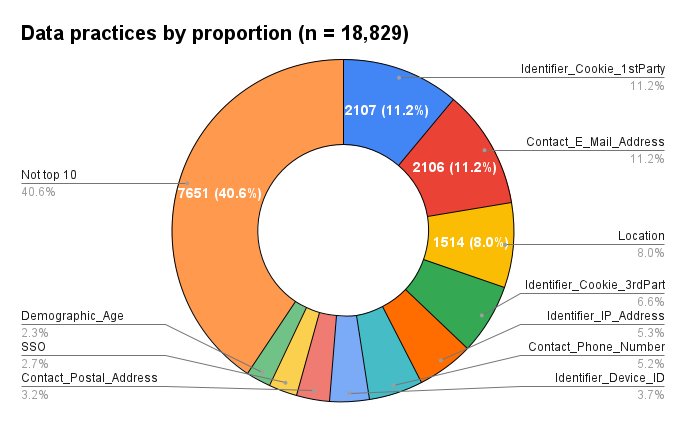
\includegraphics[width=1\textwidth]{figures/eda_data_practices.png}      
    \caption{Breakdown of data practices by proportion}
    \label{fig:eda_data_practice}
\end{figure}

\begin{table}[!ht]
	\centering
	\begin{tabular}{lrr}
		\toprule
		{} &  Mean sentence length &  Median sentence length \\
		\midrule
		count &             10.0 &               10.0 \\
		mean  &             29.8 &               25.5 \\
		std   &              2.5 &                1.9 \\
		min   &             25.4 &               22.0 \\
		25\%   &             28.7 &               24.3 \\
		50\%   &             29.1 &               25.5 \\
		75\%   &             32.0 &               26.8 \\
		max   &             33.1 &               28.0 \\
		\bottomrule
	\end{tabular}
	\caption{Summary statistics of top 10 occurring practices.}
	\label{tab:summary_top_10_practices}
\end{table}

\begin{figure}[!ht]
	\centering
	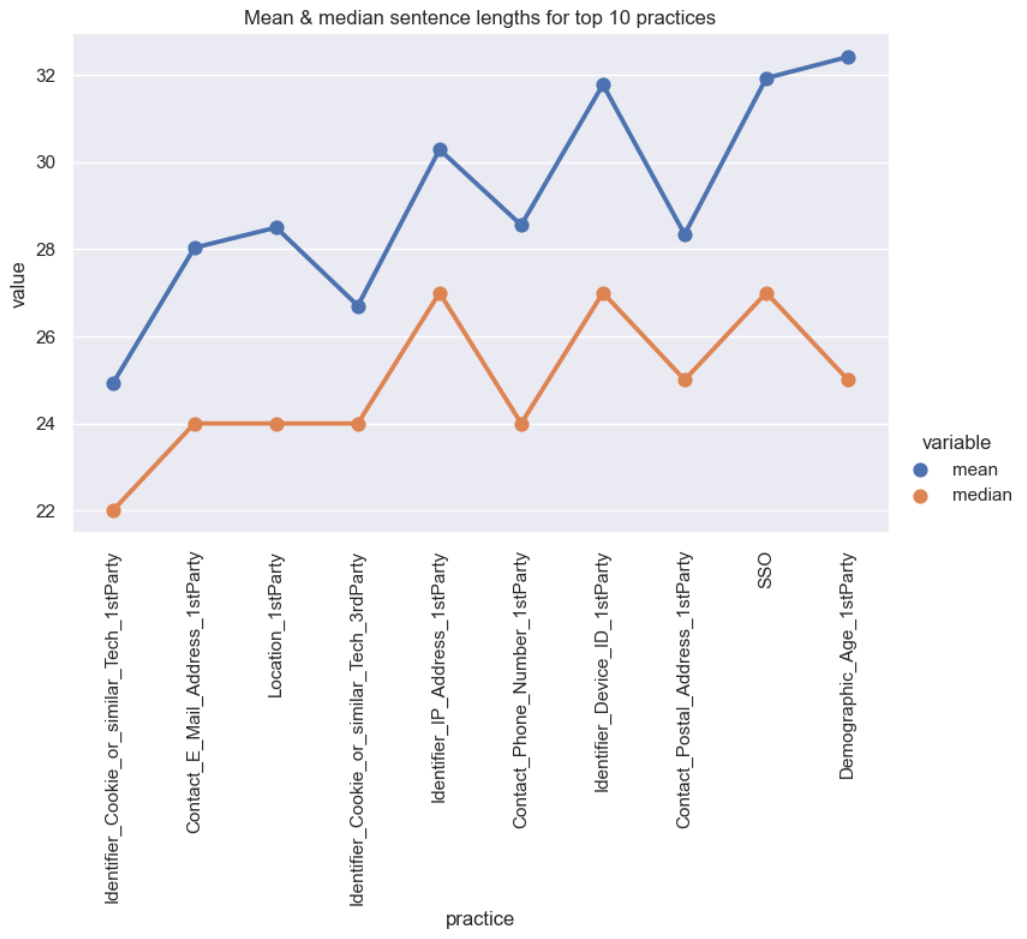
\includegraphics[width=1\textwidth]{figures/eda_mean_median.png}      
    \caption{Mean and median sentence length}
    \label{fig:graph_sentence_length}
\end{figure}


\begin{figure}[!ht]
	\begin{subfigure}[t]{.5\linewidth}
	  \centering
	  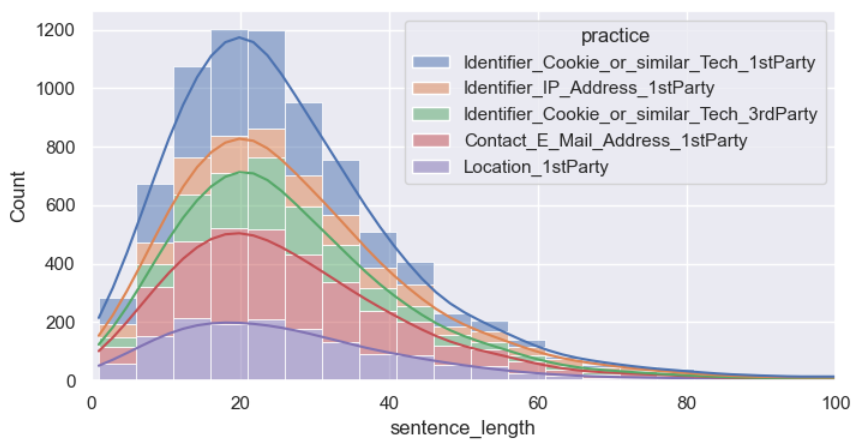
\includegraphics[width=1\linewidth]{figures/hist_eda.png}
	  \caption{Histogram of top 5 practices}
	  \label{fig:hist}
	\end{subfigure}
	\hfill
	\begin{subfigure}[t]{.5\linewidth}
		\centering
		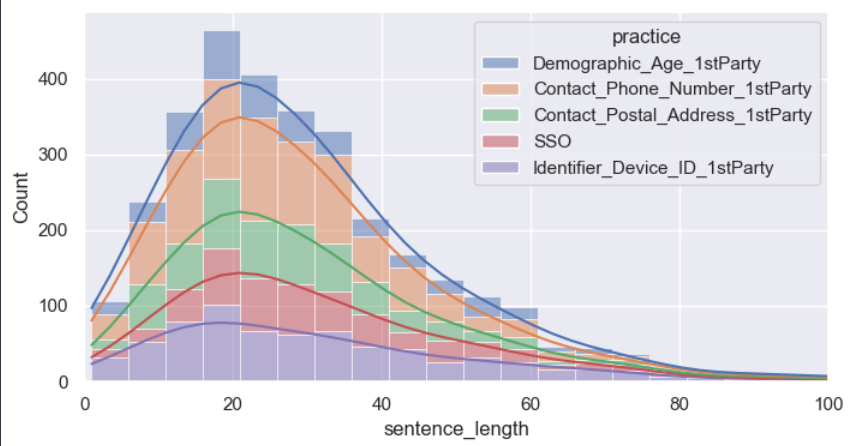
\includegraphics[width=1\linewidth]{figures/hist_eda_2.png}
		\caption{Histogram of next top 5 practices}
		\label{fig:hist_2}
	\end{subfigure}
	\medskip
	\begin{subfigure}[b]{1\linewidth}
	  \centering
	  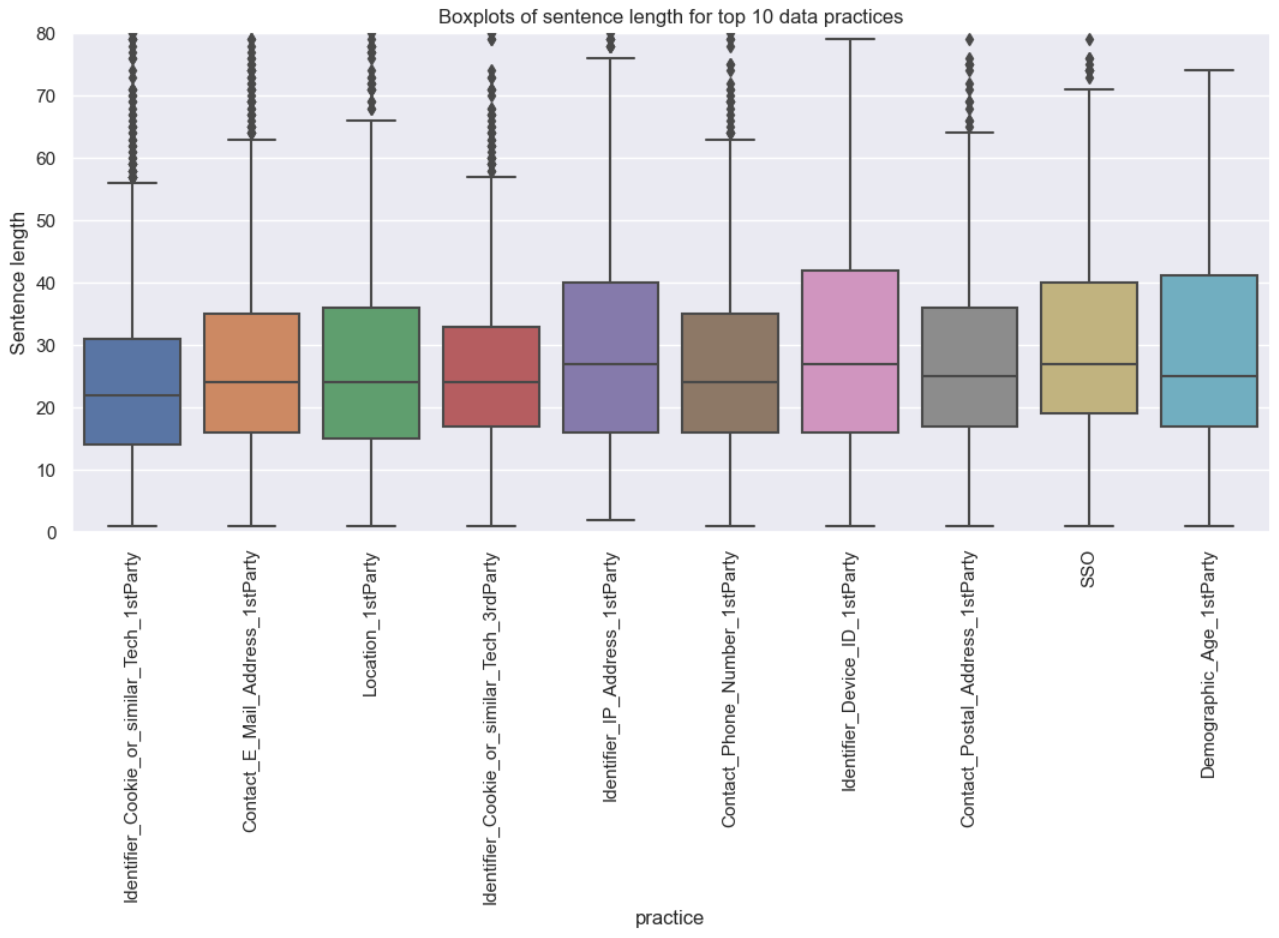
\includegraphics[width=0.85\linewidth]{figures/eda_boxplots.png}
	  \caption{Boxplots of sentence length (Practices shown in order of descending frequency)}
	  \label{fig:boxplot_top_10}
	\end{subfigure}
	\caption{Summary plots for top 10 frequently occurring data practices (note: not all outliers shown to focus on visualising IQR)}
	\label{fig:eda}
\end{figure}

With regard to top 10 frequently occurring 4-grams in the top 5 practices (Figure~\ref{fig:4_grams_sentence}), both 4-grams of \texttt{Cookie 1st Party} and \texttt{Cookie 3rd Party} contain many instances of "cookies", and it is hard to tell from the 4-grams alone whether they refer to collection of Cookies by 1st or 3rd parties. The same is seen to a lesser extent between the 4-grams of \texttt{Location} and \texttt{IP Address}, where both have instances of "IP address" and "mac address". In comparison, 4-grams of \texttt{Email} are clearly distinct from the rest of the data practices with unique tokens of "email" and "phone number".


\begin{figure}[!ht]
	\begin{subfigure}[t]{.5\textwidth}
	  \centering
	  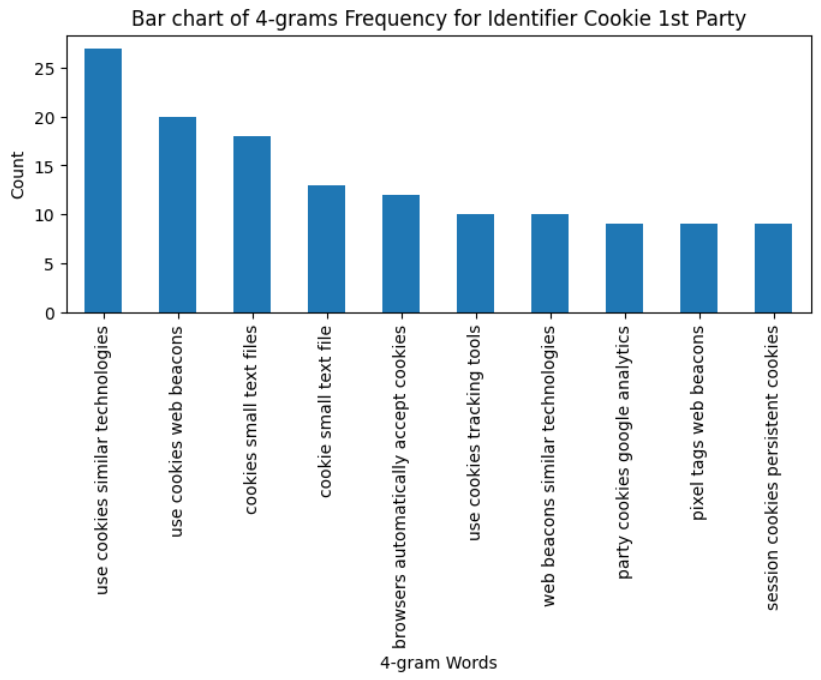
\includegraphics[width=\linewidth]{figures/4_grams_cookie_1stParty.png}
	  \caption{Identifier Cookie 1st Party}
	\end{subfigure}
	\hfill
	\begin{subfigure}[t]{.5\textwidth}
	  \centering
	  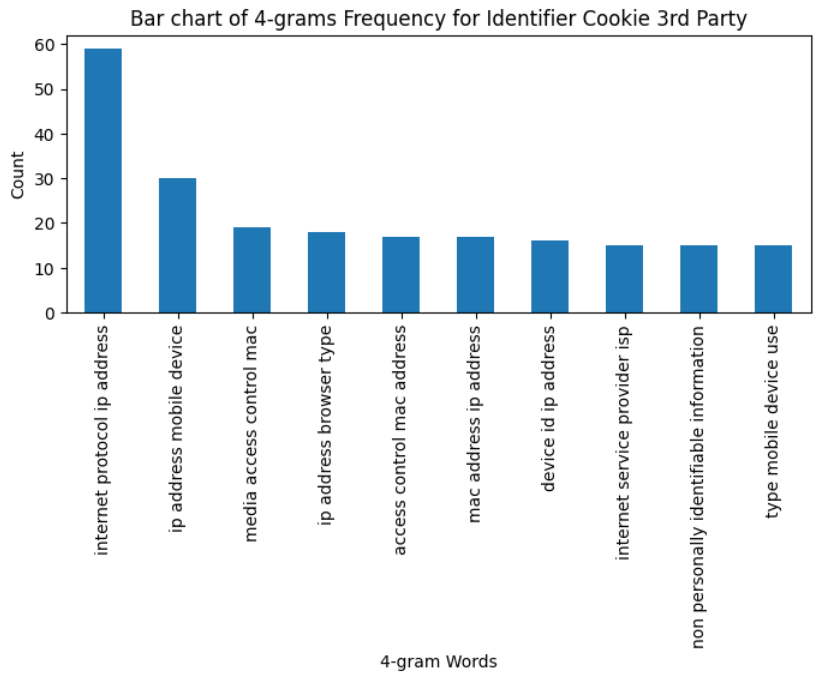
\includegraphics[width=\linewidth]{figures/4_grams_cookie_3rdParty.png}
	  \caption{Identifier Cookie 3rd Party}
	\end{subfigure}
	
	\medskip
  
	\begin{subfigure}[t]{.5\textwidth}
	  \centering
	  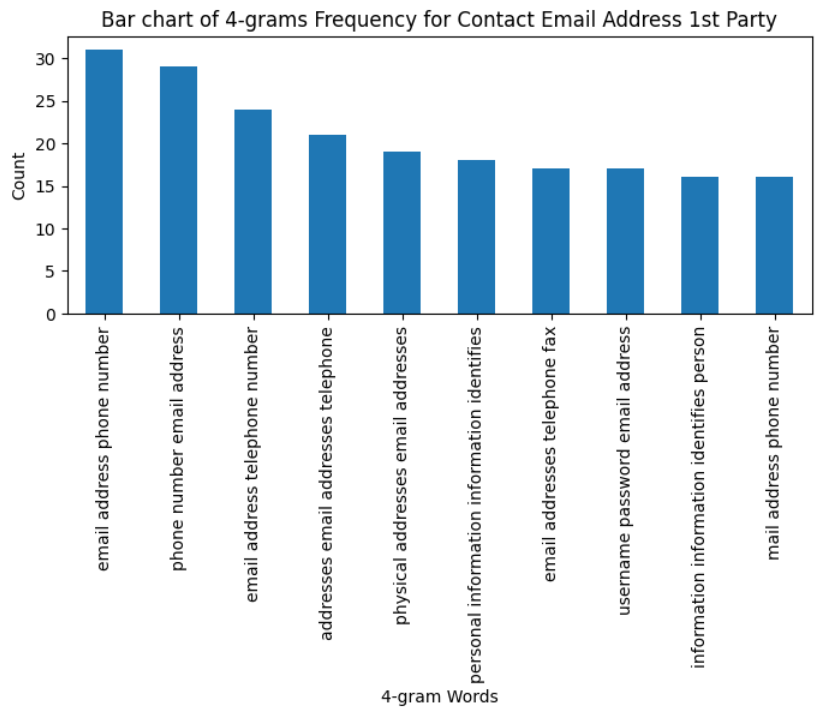
\includegraphics[width=\linewidth]{figures/4_grams_email.png}
	  \caption{Identifier Email}
	\end{subfigure}
	\hfill
	\begin{subfigure}[t]{.5\textwidth}
	  \centering
	  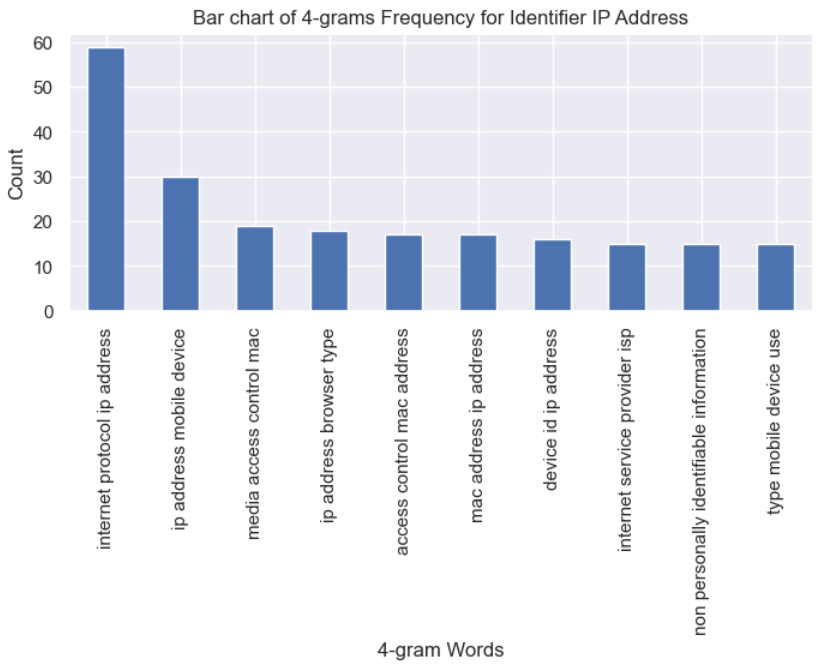
\includegraphics[width=\linewidth]{figures/4_grams_ip_address.png}
	  \caption{Identifier IP Address}
	\end{subfigure}
	\begin{subfigure}[t]{.5\textwidth}
		\centering
		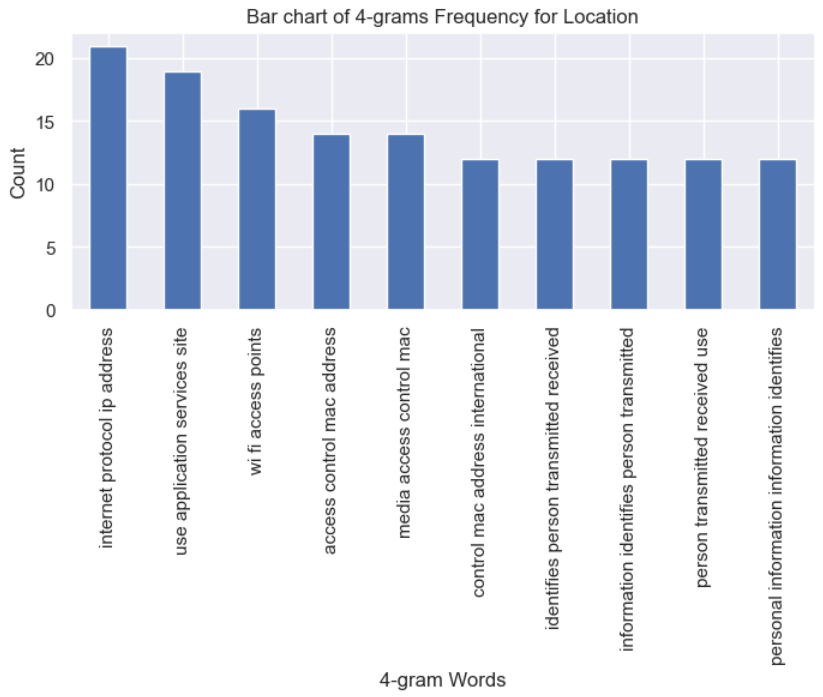
\includegraphics[width=\linewidth]{figures/4_grams_location.png}
		\caption{Location 1st Party}
	\end{subfigure}
	\caption{Top 10 most frequently occurring 4-grams in the top most frequently occurring 5 data practices at the sentence level}
	\label{fig:4_grams_sentence}
  \end{figure}

\section{Performance of classifiers for top N practices}
I compare the weighted precision, recall and F1 scores of the classifiers below. Since there is neither a high risk of identifying false positives or false negatives, F1 score is primarily used to assess the performance of the classifiers. As there is class imbalance in the top 10 data practices (Table~\ref{fig:eda_data_practice}), I focus on the weighted average F1 scores as the most important indicator of classifier performance. 

Given that there are in total 57 practices for the entire dataset but the top 10 data practices already comprise 60\% of all sentences, training classifiers on all 57 practices would likely lead to low performance. Thus, to find an optimal balance between classifier performance but still maintain realistic sentence complexity, I first assess the performance of the three classifiers using Tf-IDF for the top N (where $3 \le N \le 10$) frequently occurring practices. SVC performs the best across the metrics and across the top N frequently occurring practices (Figure~\ref{fig:top_n_practices}). This corresponds with the findings by \cite{zimmeck2019}. Also, performance of all the classifiers generally decreases with increasing $N$, which is not surprising since it is more difficult for the classifier to find a decision boundary with more classes. The following sections focuses on classifier performance of the top 5 practices as performance was still reasonable at 60\% weighted P/R/F1 scores. Also, since SGDClassifier performed the worst compared to the 2 other classifiers, I focus only on comparing logistic regression and SVC, with logistic regression as a baseline classifier.

\begin{figure}[!ht]
	\centering
	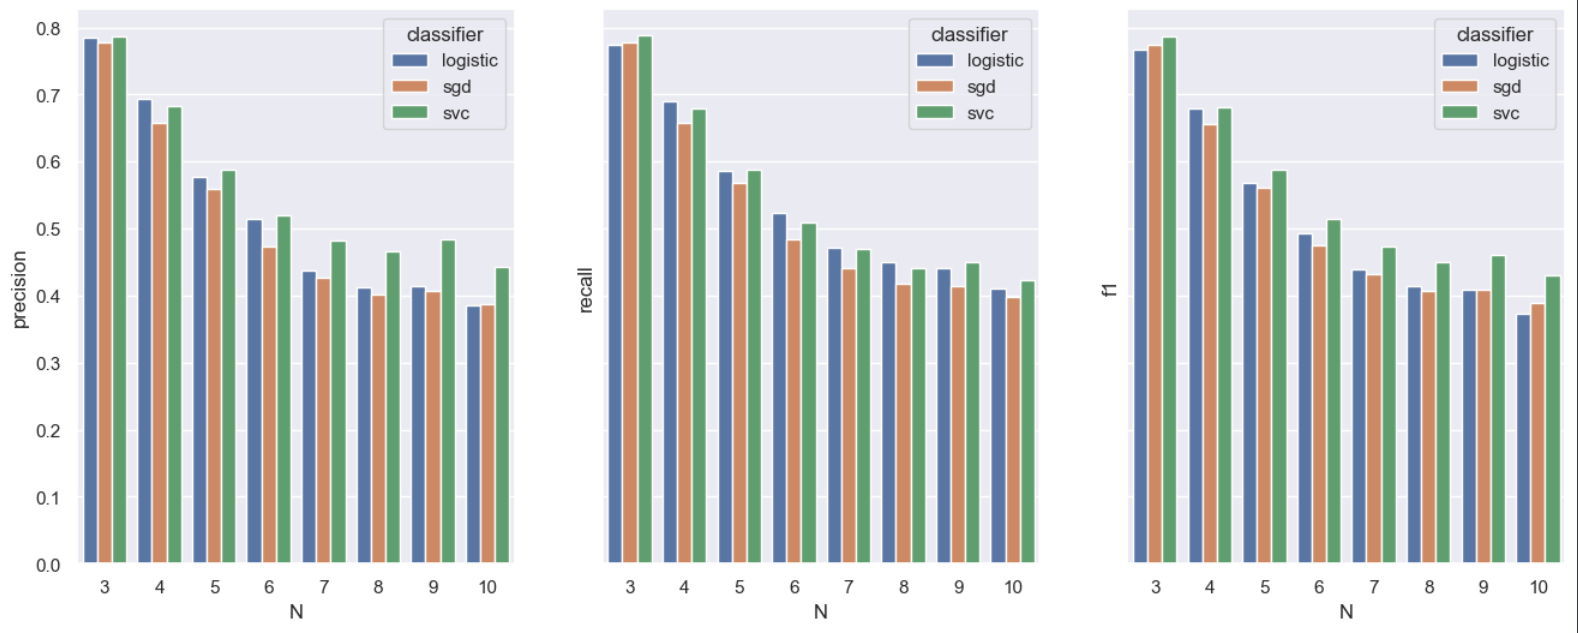
\includegraphics[width=1\textwidth]{figures/model_n_testing_sentence.png}      
    \caption{Weighted average P/R/F1 scores for top N ($3 \le N \le 10$) practices}
    \label{fig:top_n_practices}
\end{figure}

\section{Performance of individual classifiers for top 5 practices}
I report the individual performance of all 4 combinations of text representations and models. With regard to P/R/F1 scores (Figure~\ref{fig:heatmaps_perf}), similarly to what \cite{zimmeck2019} found, SVC + Tf-IDF provided the best overall performance with the weighted average at 66\%. This is quite a significant performance difference from the lowest performing model, logistic regression + GloVe at 54\%. Specifically for \texttt{Cookie 1st Party}, both logistic regression + Tf-IDF and SVC + Tf-IDF performed similarly at 68\% F1, but SVC + Tf-IDF had a more balanced performance across precision and recall. With regard to the ROC curves (Figure~\ref{fig:roc_curve}), looking at the micro-averaged AUC, the classifiers all performed similarly well within a small difference of 0.03, and similarly for \texttt{Cookie 1st Party}, the difference in AUC was 0.02. GloVe embeddings seem to cause a greater variance when comparing the AUC for each class. For instance, the difference between the highest and lowest AUC for logistic regression + GloVe is $0.89 - 0.77 = 0.12$, while for logistic regression + Tf-IDF it was $0.91 - 0.85 = 0.06$.

Overall, these performance figures confirm that SVC is the better performing model, though the performance difference between the benchmark logistic regression model and SVC is not that significant (from 62\% to 66\% weighted average F1). It is also interesting to note that GloVe embeddings performed worse and caused higher variance in performance compared to Tf-IDF regardless of the model used, when GloVe is the more sophisticated text representation that can capture some semantic meaning of the tokens. These results correspond with a study measuring performance of supervised machine learning for classification tasks using generalised text datasets \cite{hsu2020}, where LinearSVC followed by logistic regression were the highest performing models.


\begin{figure}[!ht]
	\begin{subfigure}[t]{.5\textwidth}
	  \centering
	  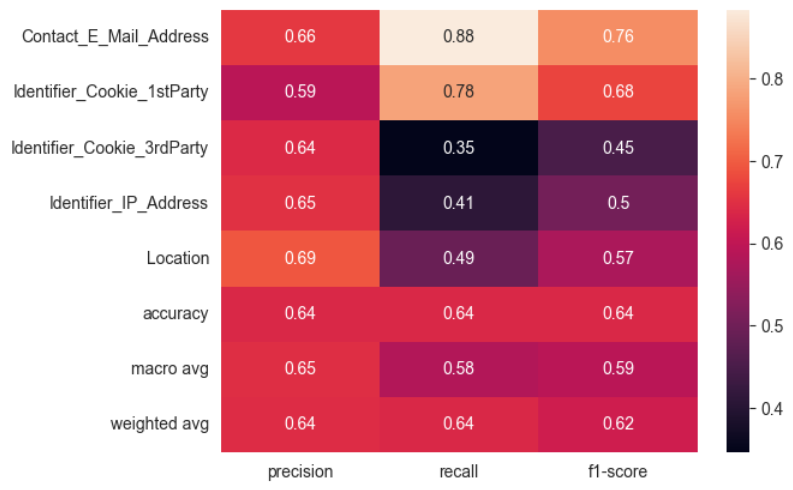
\includegraphics[width=\linewidth]{figures/heatmap_log_tfidf.png}
	  \caption{Logistic regression + TfIDF}
	\end{subfigure}
	\hfill
	\begin{subfigure}[t]{.5\textwidth}
	  \centering
	  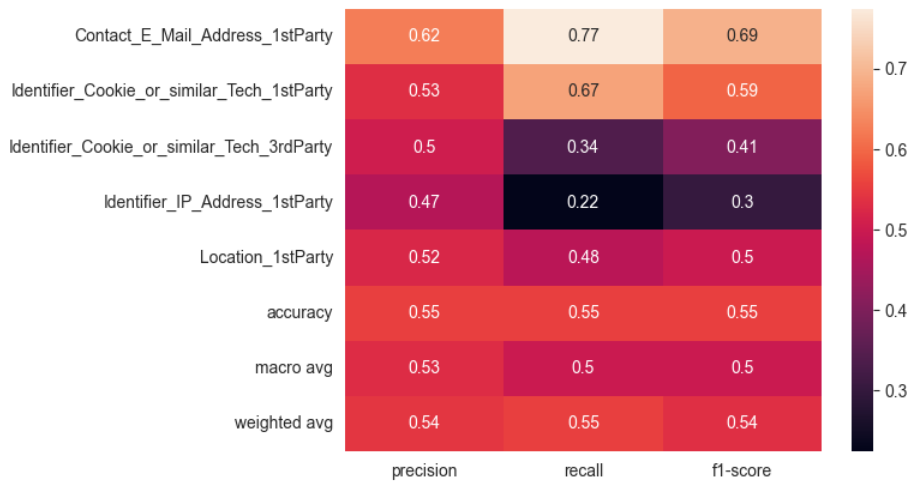
\includegraphics[width=\linewidth]{figures/heatmap_log_glove.png}
	  \caption{Logistic regression + GloVe}
	\end{subfigure}
	
	\medskip
  
	\begin{subfigure}[t]{.5\textwidth}
	  \centering
	  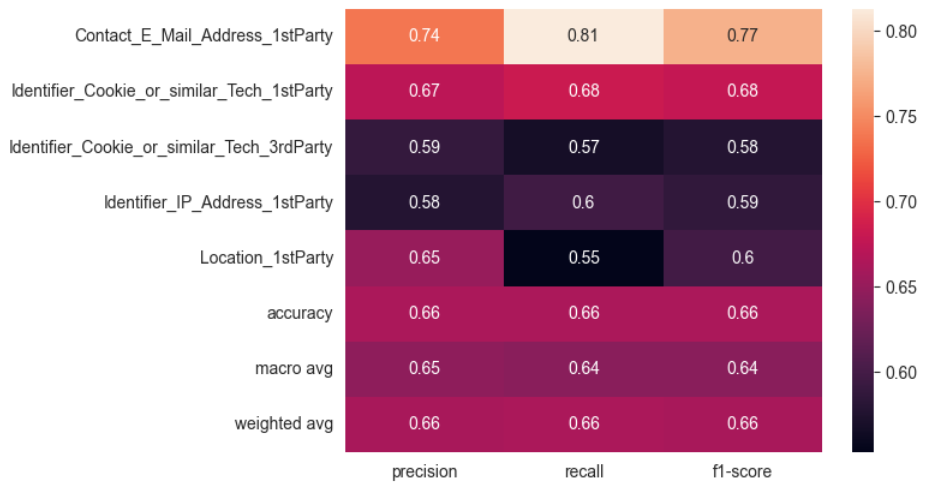
\includegraphics[width=\linewidth]{figures/heatmap_svc_tfidf.png}
	  \caption{SVC + TfIDF}
	\end{subfigure}
	\hfill
	\begin{subfigure}[t]{.5\textwidth}
	  \centering
	  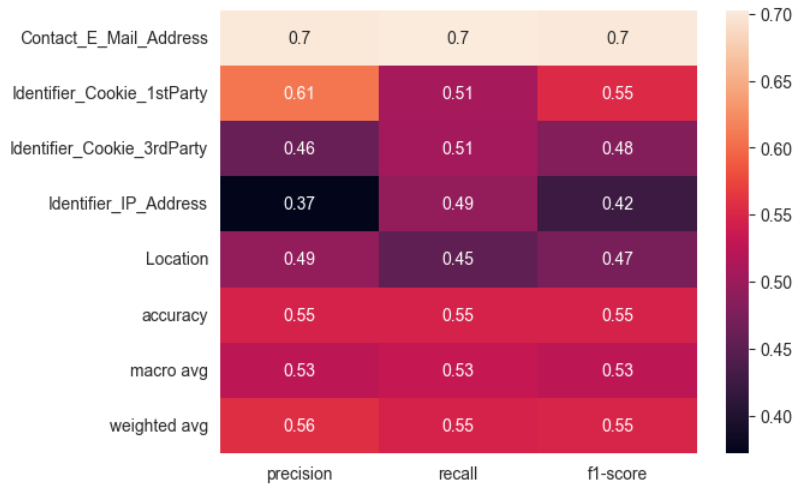
\includegraphics[width=\linewidth]{figures/heatmap_svc_glove.png}
	  \caption{SVC + GloVe}
	\end{subfigure}
	\caption{Performance heatmaps of the 4 classifiers (averaged over 5-fold cross validation)}
	\label{fig:heatmaps_perf}
  \end{figure}

\begin{figure}[!ht]
	\begin{subfigure}[t]{.5\textwidth}
	  \centering
	  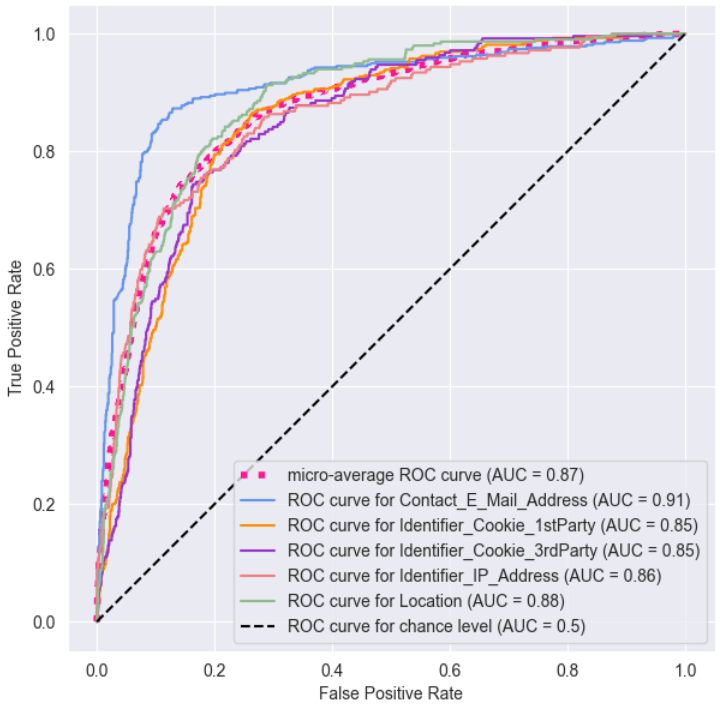
\includegraphics[width=\linewidth]{figures/roc_logistic_tfidf.png}
	  \caption{Logistic regression + TfIDF}
	\end{subfigure}
	\hfill
	\begin{subfigure}[t]{.5\textwidth}
	  \centering
	  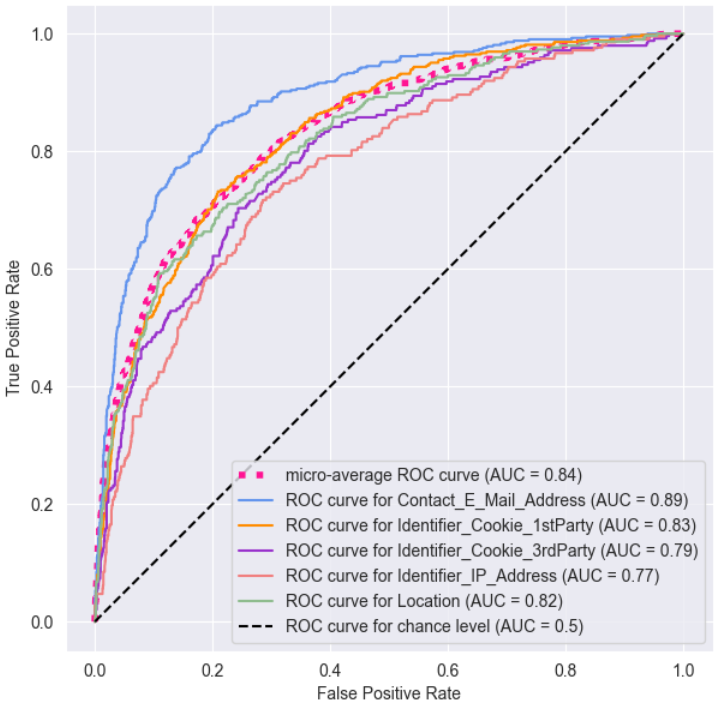
\includegraphics[width=\linewidth]{figures/roc_logistic_glove.png}
	  \caption{Logistic regression + GloVe}
	\end{subfigure}
	
	\medskip
  
	\begin{subfigure}[t]{.5\textwidth}
	  \centering
	  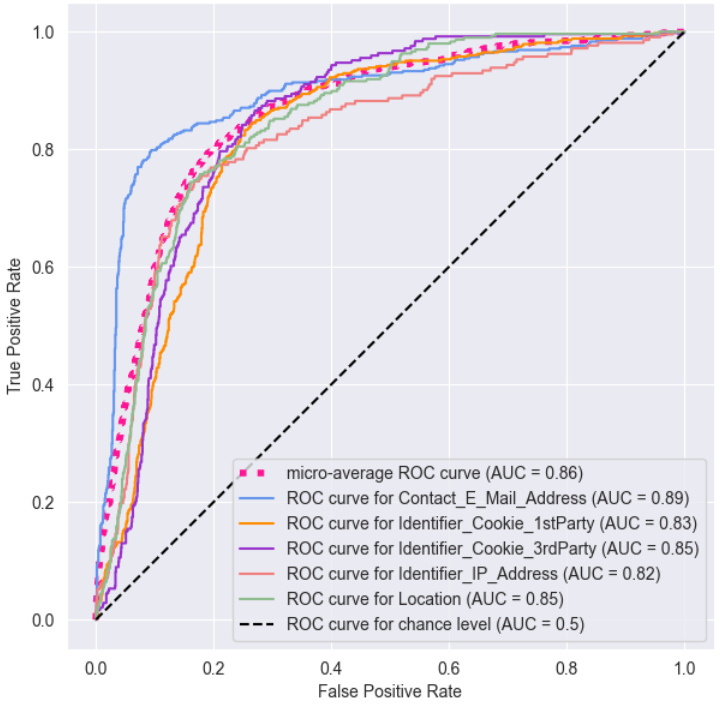
\includegraphics[width=\linewidth]{figures/roc_svc_tfidf.png}
	  \caption{SVC + TfIDF}
	\end{subfigure}
	\hfill
	\begin{subfigure}[t]{.5\textwidth}
	  \centering
	  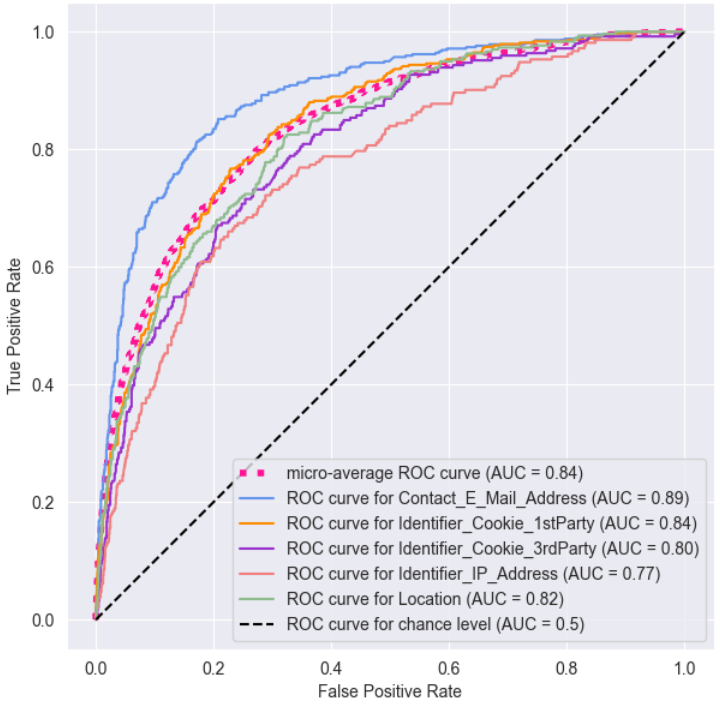
\includegraphics[width=\linewidth]{figures/roc_svc_glove.png}
	  \caption{SVC + GloVe}
	\end{subfigure}
	\caption{Multiclass Receiver Operating Characteristic (ROC) Curve of the 5 data practices for each classifier}
	\label{fig:roc_curve}
  \end{figure}


% 	\begin{table}[!ht]
% 		\resizebox{\textwidth}{!}{
% 		\begin{tabular}{lrrrr}
% 		\toprule
% 								practice &  counts &  sentence\_length\_mean &  sentence\_length\_median &  counts\_percentage \\
% 		\midrule
% 		Identifier\_Mobile\_Carrier\_3rdParty &      35 &             47.1 &                    30.0 &           0.19\% \\
% 					Contact\_ZIP\_3rdParty &      34 &             40.2 &                    41.0 &           0.18\% \\
% 		Identifier\_SSID\_BSSID\_1stParty &      33 &             28.1 &                    24.0 &           0.18\% \\
% 			  Contact\_Password\_3rdParty &      33 &             24.2 &                    20.0 &           0.18\% \\
% 					Contact\_City\_3rdParty &      24 &             180 &                    14.0 &           0.13\% \\
% 		Contact\_Address\_Book\_3rdParty &      17 &             39.6 &                    34.0 &           0.1\% \\
% 			  Identifier\_IMSI\_1stParty &      13 &             48.2 &                    44.0 &           0.07\% \\
% 		Identifier\_SIM\_Serial\_3rdParty &       5 &             41.2 &                    54.0 &           0.03\% \\
% 			  Identifier\_IMSI\_3rdParty &       4 &             54.3 &                    47.5 &           0.02\% \\
% 		Identifier\_SSID\_BSSID\_3rdParty &       2 &             65.5 &                    65.5 &           0.01\% \\
% 		\bottomrule
% 	\end{tabular}
% 	}
% 	\caption{Summary statistics for bottom 10 frequently occurring practices.}
% 	\label{tab:bottom_10_sentence}
% \end{table}


% \begin{table}[!ht]
% 	\resizebox{\textwidth}{!}{
% 		\begin{tabular}{lllll}
% 		\hline
% 		\multicolumn{1}{|l|}{\textbf{Data Practice}}          & \multicolumn{1}{l|}{\textbf{Precision}} & \multicolumn{1}{l|}{\textbf{Recall}} & \multicolumn{1}{l|}{\textbf{F1}} & \multicolumn{1}{l|}{\textbf{Support}} \\ \hline
% 		\multicolumn{1}{|l|}{Contact Email Address 1st Party} & \multicolumn{1}{l|}{0.66}               & \multicolumn{1}{l|}{0.88}            & \multicolumn{1}{l|}{0.76}        & \multicolumn{1}{l|}{2106}              \\ \hline
% 		\multicolumn{1}{|l|}{Identifier Cookie 1st Party}    & \multicolumn{1}{l|}{0.59}               & \multicolumn{1}{l|}{0.78}            & \multicolumn{1}{l|}{0.68}        & \multicolumn{1}{l|}{2107}              \\ \hline
% 		\multicolumn{1}{|l|}{Identifier Cookie 3rd Party}     & \multicolumn{1}{l|}{0.64}               & \multicolumn{1}{l|}{0.35}            & \multicolumn{1}{l|}{0.45}        & \multicolumn{1}{l|}{1250}              \\ \hline
% 		\multicolumn{1}{|l|}{Identifier IP Address 1st Party} & \multicolumn{1}{l|}{0.66}               & \multicolumn{1}{l|}{0.41}            & \multicolumn{1}{l|}{0.50}        & \multicolumn{1}{l|}{1005}              \\ \hline
% 		\multicolumn{1}{|l|}{Location 1st Party}              & \multicolumn{1}{l|}{0.69}               & \multicolumn{1}{l|}{0.49}            & \multicolumn{1}{l|}{0.57}        & \multicolumn{1}{l|}{1514}              \\ \hline
% 																&                                         &                                      &                                  &                                       \\ \hline
% 		\multicolumn{1}{|l|}{\textbf{accuracy}}               & \multicolumn{1}{l|}{}                   & \multicolumn{1}{l|}{}                & \multicolumn{1}{l|}{0.64}        & \multicolumn{1}{l|}{7982}             \\ \hline
% 		\multicolumn{1}{|l|}{\textbf{macro avg}}              & \multicolumn{1}{l|}{0.65}               & \multicolumn{1}{l|}{0.58}            & \multicolumn{1}{l|}{0.59}        & \multicolumn{1}{l|}{7982}             \\ \hline
% 		\multicolumn{1}{|l|}{\textbf{weighted avg}}           & \multicolumn{1}{l|}{0.64}               & \multicolumn{1}{l|}{0.64}            & \multicolumn{1}{l|}{0.62}        & \multicolumn{1}{l|}{7982}             \\ \hline
% 		\end{tabular}
% 	}
% 	\caption{Logistic regression + Tf-IDF}
% 	\label{tab:lr+tfidf}
% \end{table}


% \begin{table}[!ht]
% 	\resizebox{\textwidth}{!}{
% 		\begin{tabular}{lllll}
% 		\hline
% 		\multicolumn{1}{|l|}{\textbf{Data Practice}}          & \multicolumn{1}{l|}{\textbf{Precision}} & \multicolumn{1}{l|}{\textbf{Recall}} & \multicolumn{1}{l|}{\textbf{F1}} & \multicolumn{1}{l|}{\textbf{Support}} \\ \hline
% 		\multicolumn{1}{|l|}{Contact Email Address 1st Party} & \multicolumn{1}{l|}{0.62}               & \multicolumn{1}{l|}{0.77}            & \multicolumn{1}{l|}{0.70}        & \multicolumn{1}{l|}{2106}              \\ \hline
% 		\multicolumn{1}{|l|}{Identifier Cookie 1st Party}    & \multicolumn{1}{l|}{0.53}               & \multicolumn{1}{l|}{0.67}            & \multicolumn{1}{l|}{0.59}        & \multicolumn{1}{l|}{2107}              \\ \hline
% 		\multicolumn{1}{|l|}{Identifier Cookie 3rd Party}     & \multicolumn{1}{l|}{0.50}               & \multicolumn{1}{l|}{0.34}            & \multicolumn{1}{l|}{0.41}        & \multicolumn{1}{l|}{1250}              \\ \hline
% 		\multicolumn{1}{|l|}{Identifier IP Address 1st Party} & \multicolumn{1}{l|}{0.47}               & \multicolumn{1}{l|}{0.22}            & \multicolumn{1}{l|}{0.30}        & \multicolumn{1}{l|}{1005}              \\ \hline
% 		\multicolumn{1}{|l|}{Location 1st Party}              & \multicolumn{1}{l|}{0.52}               & \multicolumn{1}{l|}{0.48}            & \multicolumn{1}{l|}{0.50}        & \multicolumn{1}{l|}{1514}              \\ \hline
% 																&                                         &                                      &                                  &                                       \\ \hline
% 		\multicolumn{1}{|l|}{\textbf{accuracy}}               & \multicolumn{1}{l|}{}                   & \multicolumn{1}{l|}{}                & \multicolumn{1}{l|}{0.55}        & \multicolumn{1}{l|}{7982}             \\ \hline
% 		\multicolumn{1}{|l|}{\textbf{macro avg}}              & \multicolumn{1}{l|}{0.53}               & \multicolumn{1}{l|}{0.50}            & \multicolumn{1}{l|}{0.50}        & \multicolumn{1}{l|}{7982}             \\ \hline
% 		\multicolumn{1}{|l|}{\textbf{weighted avg}}           & \multicolumn{1}{l|}{0.54}               & \multicolumn{1}{l|}{0.55}            & \multicolumn{1}{l|}{0.54}        & \multicolumn{1}{l|}{7982}             \\ \hline
% 		\end{tabular}
% 	}
% 	\caption{Logistic regression + GloVe embeddings}
% 	\label{tab:lr+glove}
% \end{table}


% \begin{table}[!ht]
% 	\resizebox{\textwidth}{!}{
% 	\begin{tabular}{lllll}
% 		\hline
% 		\multicolumn{1}{|l|}{\textbf{Data Practice}}          & \multicolumn{1}{l|}{\textbf{Precision}} & \multicolumn{1}{l|}{\textbf{Recall}} & \multicolumn{1}{l|}{\textbf{F1}} & \multicolumn{1}{l|}{\textbf{Support}} \\ \hline
% 		\multicolumn{1}{|l|}{Contact Email Address 1st Party} & \multicolumn{1}{l|}{0.74}               & \multicolumn{1}{l|}{0.81}            & \multicolumn{1}{l|}{0.77}        & \multicolumn{1}{l|}{2106}              \\ \hline
% 		\multicolumn{1}{|l|}{Identifier Cookie 1st Party}     & \multicolumn{1}{l|}{0.67}               & \multicolumn{1}{l|}{0.68}            & \multicolumn{1}{l|}{0.68}        & \multicolumn{1}{l|}{2107}              \\ \hline
% 		\multicolumn{1}{|l|}{Identifier Cookie 3rd Party}     & \multicolumn{1}{l|}{0.59}               & \multicolumn{1}{l|}{0.57}            & \multicolumn{1}{l|}{0.58}        & \multicolumn{1}{l|}{1250}              \\ \hline
% 		\multicolumn{1}{|l|}{Identifier IP Address 1st Party} & \multicolumn{1}{l|}{0.58}               & \multicolumn{1}{l|}{0.60}            & \multicolumn{1}{l|}{0.59}        & \multicolumn{1}{l|}{1005}              \\ \hline
% 		\multicolumn{1}{|l|}{Location 1st Party}              & \multicolumn{1}{l|}{0.65}               & \multicolumn{1}{l|}{0.55}            & \multicolumn{1}{l|}{0.60}        & \multicolumn{1}{l|}{1514}              \\ \hline
% 																&                                         &                                      &                                  &                                       \\ \hline
% 		\multicolumn{1}{|l|}{\textbf{accuracy}}               & \multicolumn{1}{l|}{}                   & \multicolumn{1}{l|}{}                & \multicolumn{1}{l|}{0.66}        & \multicolumn{1}{l|}{7982}             \\ \hline
% 		\multicolumn{1}{|l|}{\textbf{macro avg}}              & \multicolumn{1}{l|}{0.65}               & \multicolumn{1}{l|}{0.64}            & \multicolumn{1}{l|}{0.64}        & \multicolumn{1}{l|}{7982}             \\ \hline
% 		\multicolumn{1}{|l|}{\textbf{weighted avg}}           & \multicolumn{1}{l|}{0.66}               & \multicolumn{1}{l|}{0.66}            & \multicolumn{1}{l|}{0.66}        & \multicolumn{1}{l|}{7982}             \\ \hline
% 		\end{tabular}
% 	}
% 	\caption{SVC + Tf-IDF}
% 	\label{tab:svc+tfidf}
% \end{table}

% \begin{table}[!ht]
% 	\resizebox{\textwidth}{!}{
% 	\begin{tabular}{lllll}
% 		\hline
% 		\multicolumn{1}{|l|}{\textbf{Data Practice}}          & \multicolumn{1}{l|}{\textbf{Precision}} & \multicolumn{1}{l|}{\textbf{Recall}} & \multicolumn{1}{l|}{\textbf{F1}} & \multicolumn{1}{l|}{\textbf{Support}} \\ \hline
% 		\multicolumn{1}{|l|}{Contact Email Address 1st Party} & \multicolumn{1}{l|}{0.70}               & \multicolumn{1}{l|}{0.70}            & \multicolumn{1}{l|}{0.70}        & \multicolumn{1}{l|}{2106}              \\ \hline
% 		\multicolumn{1}{|l|}{Identifier Cookie 1st Party}     & \multicolumn{1}{l|}{0.61}               & \multicolumn{1}{l|}{0.51}            & \multicolumn{1}{l|}{0.55}        & \multicolumn{1}{l|}{2107}              \\ \hline
% 		\multicolumn{1}{|l|}{Identifier Cookie 3rd Party}     & \multicolumn{1}{l|}{0.46}               & \multicolumn{1}{l|}{0.51}            & \multicolumn{1}{l|}{0.48}        & \multicolumn{1}{l|}{1250}              \\ \hline
% 		\multicolumn{1}{|l|}{Identifier IP Address 1st Party} & \multicolumn{1}{l|}{0.37}               & \multicolumn{1}{l|}{0.49}            & \multicolumn{1}{l|}{0.42}        & \multicolumn{1}{l|}{1005}              \\ \hline
% 		\multicolumn{1}{|l|}{Location 1st Party}              & \multicolumn{1}{l|}{0.49}               & \multicolumn{1}{l|}{0.45}            & \multicolumn{1}{l|}{0.47}        & \multicolumn{1}{l|}{1514}              \\ \hline
% 																&                                         &                                      &                                  &                                       \\ \hline
% 		\multicolumn{1}{|l|}{\textbf{accuracy}}               & \multicolumn{1}{l|}{}                   & \multicolumn{1}{l|}{}                & \multicolumn{1}{l|}{0.55}        & \multicolumn{1}{l|}{7982}             \\ \hline
% 		\multicolumn{1}{|l|}{\textbf{macro avg}}              & \multicolumn{1}{l|}{0.53}               & \multicolumn{1}{l|}{0.53}            & \multicolumn{1}{l|}{0.53}        & \multicolumn{1}{l|}{7982}             \\ \hline
% 		\multicolumn{1}{|l|}{\textbf{weighted avg}}           & \multicolumn{1}{l|}{0.56}               & \multicolumn{1}{l|}{0.55}            & \multicolumn{1}{l|}{0.55}        & \multicolumn{1}{l|}{7982}             \\ \hline
% 	\end{tabular}
% 	}
% 	\caption{SVC + GloVe embeddings}
% 	\label{tab:svc+glove}
% \end{table}
% Chapter Template
\chapter{Discussion of survey results}
\label{chapter4}

In total, 31 responses were collected. The majority of respondents majored in law (58\%) vs non-law (42\%) respondents (Figure~\ref{fig:demo_1}). Except for the questions relating to subject matter expertise (data privacy and AI), the level of agreement of law vs non-law respondents about their beliefs relating to data privacy and AI were about the same (Figure~\ref{fig:demo_3}). Law respondents had less expertise in AI, while conversely, non-law respondents had less experience with data privacy. Across all respondents, while they rated that decisions by AI could be a risk to society (about 4), they also agreed that decisions by AI could be equally useful. This perhaps suggests that the respondents think the balance between "usefulness" and "risks" are not zero-sum; AI could be very helpful in solving problems, but at the same time users should be cognisant of the risks.

I mainly used sentences annotated as \texttt{Identifier Cookie 1st Party} to produce explanations for the survey. This is because the class performance of \texttt{Identifier Cookie 1st Party} performed relatively well, and has the highest number of instances in the dataset which provides a large variety of drafting styles.

\begin{figure}[!ht]
  \centering
  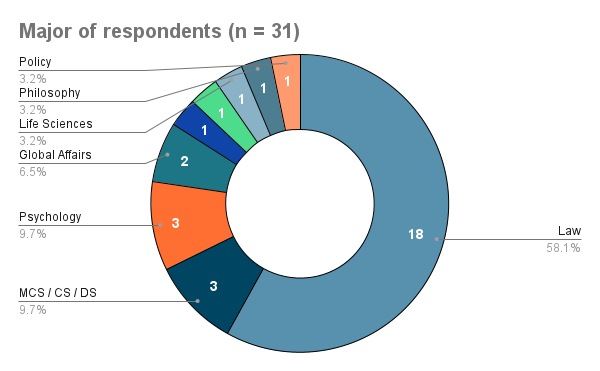
\includegraphics[width=0.85\linewidth]{figures/major_respondents.png}
  \caption{Breakdown of respondents' expertise by major}
  \label{fig:demo_1}
\end{figure}

% \begin{table}[!ht]
%     \resizebox{\textwidth}{!}{
%     \begin{tabular}{|p{0.45\linewidth}|l|l|}
%     \hline
%     \textbf{Major / Expected major}                    & \textbf{Count} & \textbf{Percentage of total (\%)} \\ \hline
%     Law                                                & 18             & 58                                \\ \hline
%     MCS / Computer Science / Data Science / Statistics & 3              & 9.7                               \\ \hline
%     Psychology                                         & 3              & 9.7                               \\ \hline
%     Global Affairs / Political Science                 & 2              & 6.5                               \\ \hline
%     Environmental Studies                              & 1              & 3.2                               \\ \hline
%     Economics                                          & 1              & 3.2                               \\ \hline
%     Life Sciences                                      & 1              & 3.2                               \\ \hline
%     Philosophy                                         & 1              & 3.2                               \\ \hline
%     Policy                                             & 1              & 3.2                               \\ \hline
%     \end{tabular}
%     }
%     \caption{Demographic breakdown of respondents according to academic discipline}
%     \label{tab:demo_1}
% \end{table}

\begin{figure}[!ht]
    \begin{subfigure}[b]{1\textwidth}
      \centering
      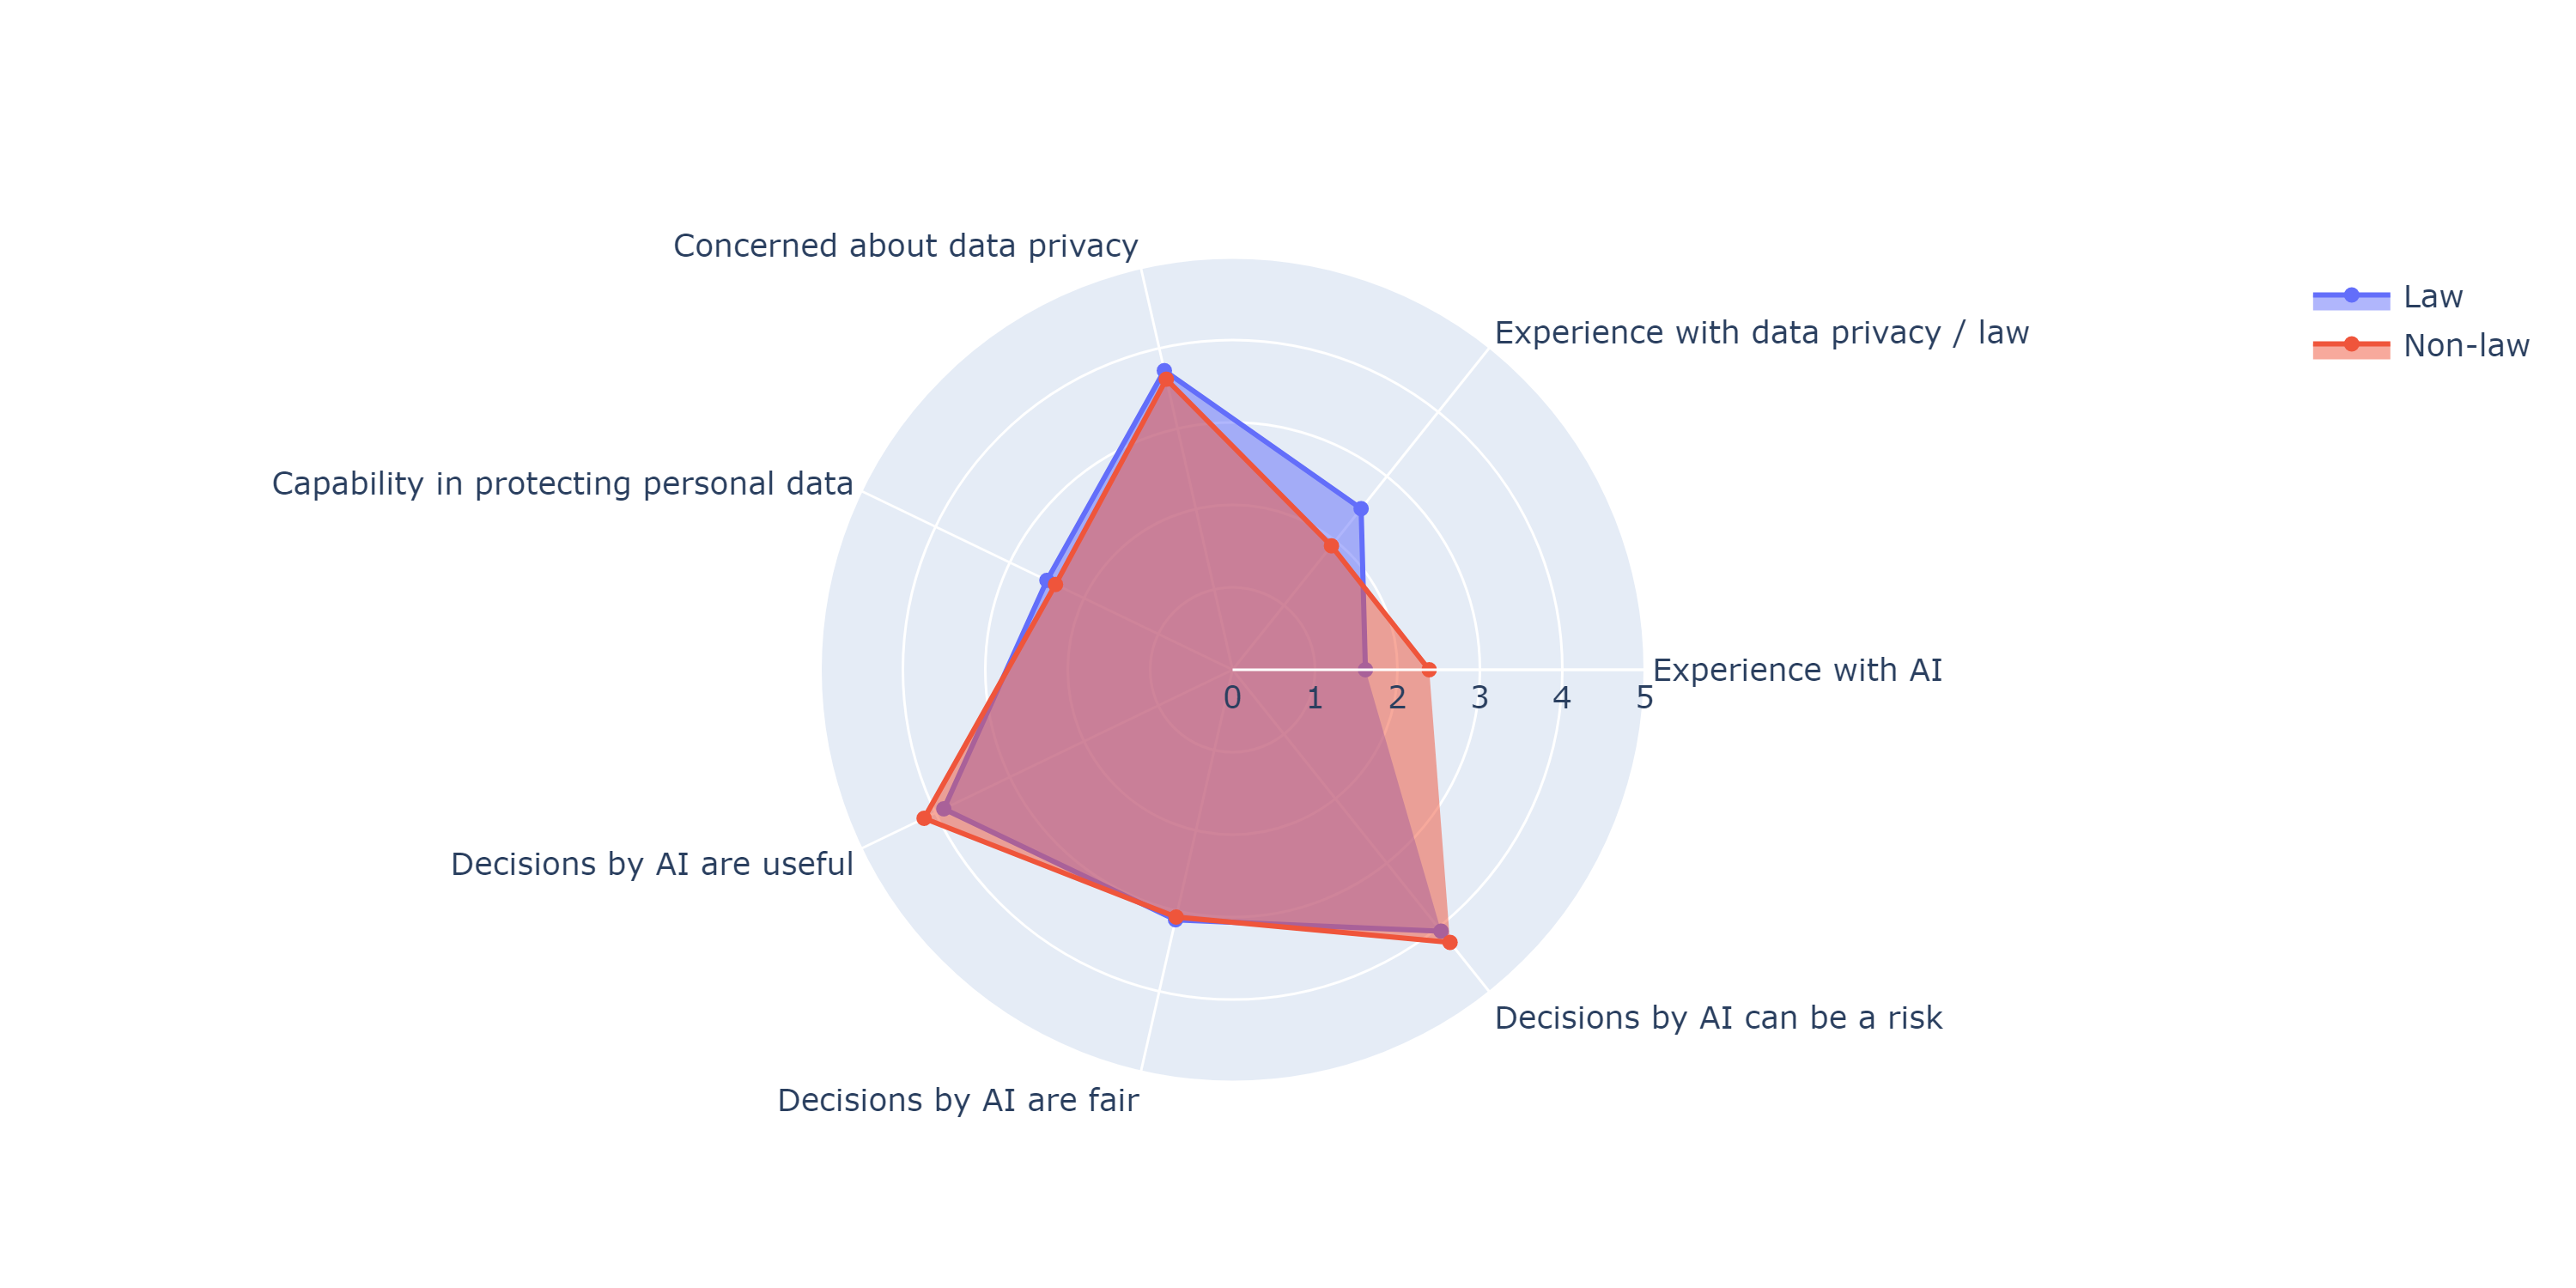
\includegraphics[width=1\linewidth]{figures/demo_3.png}
      \caption{Law vs Non-law respondents}
    \end{subfigure}
    \hfill
    \begin{subfigure}[b]{1\textwidth}
      \centering
      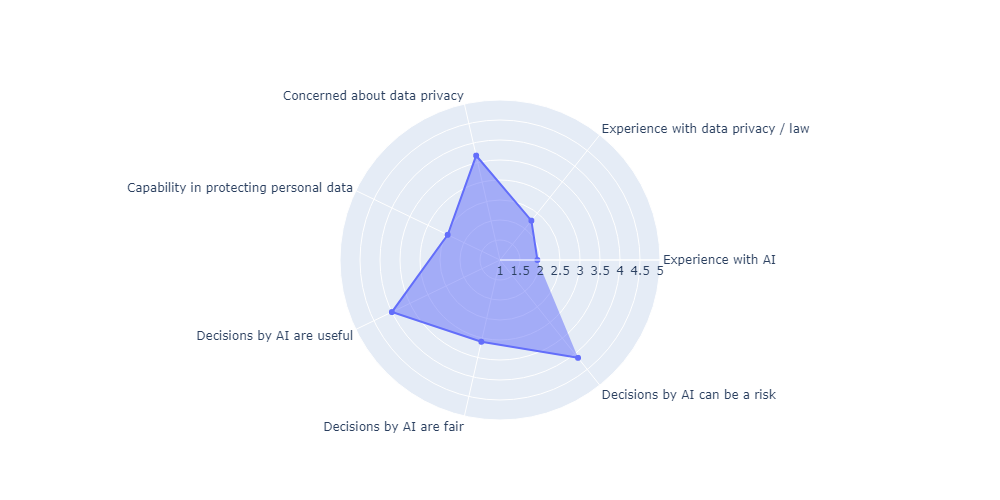
\includegraphics[width=1\linewidth]{figures/demo_4.png}
      \caption{All respondents}
    \end{subfigure}
    \caption{Mean scores of self-reported beliefs of respondents regarding AI \& data privacy. (1 = least agree, 5 = strongly agree. $n=31$)}
    \label{fig:demo_3}
\end{figure}

\section{Part 2 \& Part 6: Comparison of self-reported scores of explainability across the three contexts}
\label{sec:three_contexts_comparison}
Using the Wilcoxon Rank Sum Test, I tested for the following, setting $\alpha = 0.1$: 
\begin{align*}
    H0&: \text{There is no increase / decrease in scores after viewing the explainations.} \\
    H1&: \text{There is an increase / decrease in scores after viewing the explainations.}
\end{align*}
The 1-sided test was used to check whether the distribution underlying the difference between the initial and final paired scores was symmetric below or above 0 \cite{scipy}. Mathematically this difference can be stated as $d = i - f$, where $i$ and $f$ are the scores reported before and after viewing the explanations, and $d$ is the difference. Hence, if $d < 0$, then $i < f$ and the scores increased after viewing. Conversely, if $d > 0$, then $i > f$ and the scores decreased after viewing. p-values are reported in Table~\ref{tab:context_comparison} and~\ref{tab:context_comparison_2}. For Table~\ref{tab:context_comparison_2a} and~\ref{tab:context_comparison_2b}, I took the mean of self-reported scores across contexts, and across each metric respectively. For Table~\ref{tab:context_comparison_2c}, the self-reported scores were averaged across both context and metric. The trending in scores across the contexts are visualised in Figure~\ref{fig:part2_part6_comparison}.

\begin{table}[!ht]
    \centering
    \resizebox{\textwidth}{!}{    
    \begin{tabular}{|p{0.3\textwidth}|p{0.15\textwidth}|p{0.15\textwidth}|p{0.15\textwidth}|p{0.15\textwidth}|p{0.15\textwidth}|p{0.15\textwidth}|}
    \hline
        \textbf{Question} & \textbf{Context 1: Increase} & \textbf{Context 1: Decrease} & \textbf{Context 2: Increase} & \textbf{Context 2: Decrease} & \textbf{Context 3: Increase} & \textbf{Context 3: Decrease} \\ \hline
        \textbf{Do you think model is effective?} & \cellcolor{red!25}0.013 & 0.987 & 0.932 & \cellcolor{red!25}0.0684 & 0.856 & 0.144 \\ \hline
        \textbf{Do you think model is a fair method?} & 0.382 & 0.618 & 0.841 & 0.159 & 0.933 & \cellcolor{red!25}0.0671 \\ \hline
        \textbf{Do you think model is a risk to society?} & 0.756 & 0.244 & 0.428 & 0.572 & 0.825 & 0.175 \\ \hline
        \textbf{Do you trust the prediction of the model?} & 0.887 & 0.113 & 0.945 & \cellcolor{red!25}0.055 & 0.837 & 0.163 \\ \hline
    \end{tabular}
    }
    \caption{p-values comparing whether there was a statistically significant increase / decrease in the explainability scores before and after viewing explanations.}
    \label{tab:context_comparison}
\end{table}

\begin{table}[!ht]
    \centering
    \begin{subtable}[h]{0.45\textwidth}
      \centering  
      \begin{tabular}{|l|l|}
        \hline
            \textbf{Context} & \textbf{p-value} \\ \hline
            1: Increase & 0.369 \\ \hline
            1: Decrease & 0.633 \\ \hline
            2: Increase & 0.940 \\ \hline
            2: Decrease & \cellcolor{red!25}0.060 \\ \hline
            3: Increase & 0.955 \\ \hline
            3: Decrease & \cellcolor{red!25}0.0450 \\ \hline
        \end{tabular}
        \caption{p-values by metrics, taking the mean of scores across contexts}
        \label{tab:context_comparison_2a}
    \end{subtable}
    \hfill
    \begin{subtable}[h]{0.45\textwidth}
      \centering  
      \begin{tabular}{|l|l|}
            \hline  
            \textbf{Metric}                                    & \textbf{p-value}                     \\ 
            \hline
            Effective: Increase & 0.485  \\ \hline
            Effective: Decrease & 0.515  \\ \hline
            Fair: Increase      & 0.826  \\ \hline
            Fair: Decrease      & 0.174  \\ \hline
            Risk: Increase      & 0.660  \\ \hline
            Risk : Decrease     & 0.340  \\ \hline
            Trust: Increase     & 0.953  \\ \hline
            Trust: Decrease     & \cellcolor{red!25}0.0468 \\ \hline
        \end{tabular}
        \caption{p-values by contexts, taking the mean of scores across metrics}
        \label{tab:context_comparison_2b}
    \end{subtable}
    \hfill
    \begin{subtable}[h]{0.45\textwidth}
      \centering
      \begin{tabular}{|l|l|}
        \hline
        \textbf{Increase} & \textbf{Decrease} \\ \hline
        0.844             & 0.156           \\ \hline
      \end{tabular}
    \caption{p-values taking the mean scores across contexts and metrics}
    \label{tab:context_comparison_2c}
    \end{subtable}
    \caption{p-values comparing mean scores (cells highlighted in red are statistically significant)}
    \label{tab:context_comparison_2}
\end{table}

\begin{figure}[!ht]
  \centering
  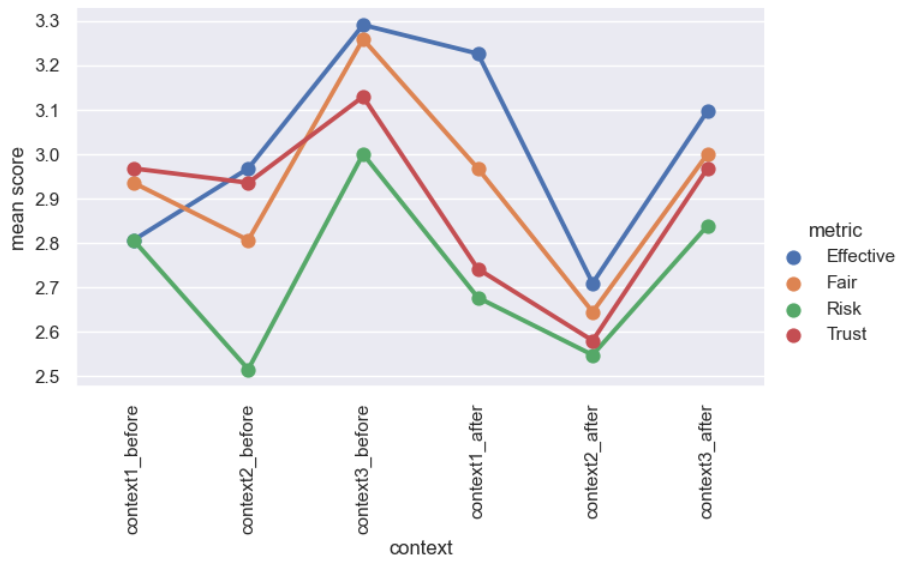
\includegraphics[width=1\linewidth]{figures/part2_part6_metric_comparison.png}
  \caption{Mean scores for each metric and each context before and after respondents viewed explanations}
  \label{fig:part2_part6_comparison}
\end{figure}


Here are the instances when $p<0.1$, and therefore $H0$ can be rejected in favour of $H1$:
\begin{enumerate}
    \item Effectiveness and trust significantly decreased for context 2 (PDPC), and fairness significantly decreased for context 3 (user). Effectiveness significantly increased for context 1 (app developer) (Table~\ref{tab:context_comparison}).
    \item There is a statistically significant decrease in explainability metrics for context 1 and 2 when comparing the mean of the scores across the metrics (Table~\ref{tab:context_comparison_2a}) and for trust across the three contexts (Table~\ref{tab:context_comparison_2b}). Interestingly, there seems to be a higher correlation between the scores of the 4 metrics specifically for context 2 and 3 after the the respondents viewed the explanations (Figure~\ref{fig:part2_part6_comparison}).
\end{enumerate}

Remember that the explanations given to respondents were deliberately chosen to demonstrate the limitations of the model. Hence, respondents were likely more cognisant of such limitations\footnote{This can also be inferred from the negative trend of interpretability and understandability as explained \hyperref[sec:interpret_understand]{below}.} when they answered the same questions again in Part 6. Here are some inferences that I draw from these observations:
\begin{enumerate}
    \item \textit{"Efficiency" is dependent on the risks of making wrong predictions (App developer, PDPC)}: The speed of automation of reading privacy policies would be the same regardless whether an app developer or PDPC uses it. However, changes in efficiency differed between the 2 contexts, suggesting that automation was not the only metric that respondents considered as part of "effectiveness". Respondents could have considered that automation was more important to app developers when balanced against the risks of making a wrong prediction, as compared to the PDPC, where the risks were too high to justify automation. Hence, the classifier is not "effective" in terms of making a legally defensible decision given that it is fallible.
    \item \textit{Classifier's interpretability is especially critical for the PDPC such that trust was affected}: Respondents could have thought that PDPC, as a regulatory body in comparison to app developers and users who are not, should fully understand and explicitly justify the decision of finding an organisation (such as an app developer) liable for breaching the PDPA. Hence, when respondents reported a drop in overall interpretability and understandability, it especially affected their trust in the logic of the classifier.
    \item \textit{Fairness is perceived in relation to the user's own interests, rather than systematic fairness}: If respondents believed that the logic of the classifier was unfair because it would unfairly discriminate against a certain style of writing data privacy policies (a kind of "systemic fairness"), respondents would also have reported a drop in fairness for the PDPC context as there would be the most expectation on a regulatory body to treat data subjects and organisations equally. However, fairness only dropped for the user and not the PDPC. This could suggest that respondents viewed the drop in fairness as not being able to get recourse for their data rights which have been violated because the classifier they are relying on for evidence to the PDPC could make wrong predictions which would affect their legal claim.
    \item \textit{Expertise of the end user of explanations affects explainability}: In relation to the overall drop in explainability metrics for the contexts of the PDPC and the user, perhaps the respondents thought that PDPC and the user did not have technical knowledge to better understand the classifier's logic beyond the explanations that were presented to them, whereas the app developer would have such technical knowledge. Hence, the lack of technical expertise of the PDPC and the user caused the drop in explainability metrics.
    \item \textit{Mismatch in expectations particularly affects trust}: In the case of trust being the only metric that significantly decreased across the contexts, this could point to a mismatch of expectations. Intuitively, if respondents do not understand how a process works, they are less likely to trust the results of that process. Perhaps respondents' expectations of AI was that AI would reason similarly to how humans would, or that AI functioned entirely objectively similar to applying a formula in Excel where it is clear how the result was obtained from the formula. Instead, the explanations provided showed that the classifier was inconsistent, sometimes relying heavily on words like "cookies" and other times not so much without any discernible reason. So respondents' expectations were not met, and this caused the overall drop in trust.
\end{enumerate}

\section{Part 3: Testing whether viewing more visualisations increased explainability}
\subsection{Analysis of the reported scores of interpret and understand}
\label{sec:interpret_understand}
There is a decreasing trend of both understandability and interpretability after viewing each explanation (Figure~\ref{fig:part3_trend}, explanations can be viewed in Figure~\ref{fig:part4_explanations}). Using the Wilcoxon Rank Sum Test, I separately tested for significant differences of understandability and interpretability, setting $\alpha = 0.1$: 

\noindent H0: There is no difference in reported interpretability / understandability between the first and last questions.

\noindent H1: There is an increase / decrease of reported interpretability / understandability between the first and last questions.

\begin{table}[!ht]
  \centering
  \begin{tabular}{l|l|l|}
  \cline{2-3}
                                                & \textbf{Increase} & \textbf{Decrease} \\ \hline
  \multicolumn{1}{|l|}{\textbf{Interpretable}} & 0.867             & 0.132             \\ \hline
  \multicolumn{1}{|l|}{\textbf{Understandable}}  & 0.999             & \cellcolor{red!25}\textless{}0.001  \\ \hline
  \end{tabular}
  \caption{p-values comparing reported understandability and interpretability between the first and last question (cells highlighted in red are statistically significant)}
  \label{tab:p_values_interpret_understand}
\end{table}

\begin{figure}[!ht]
  \centering
  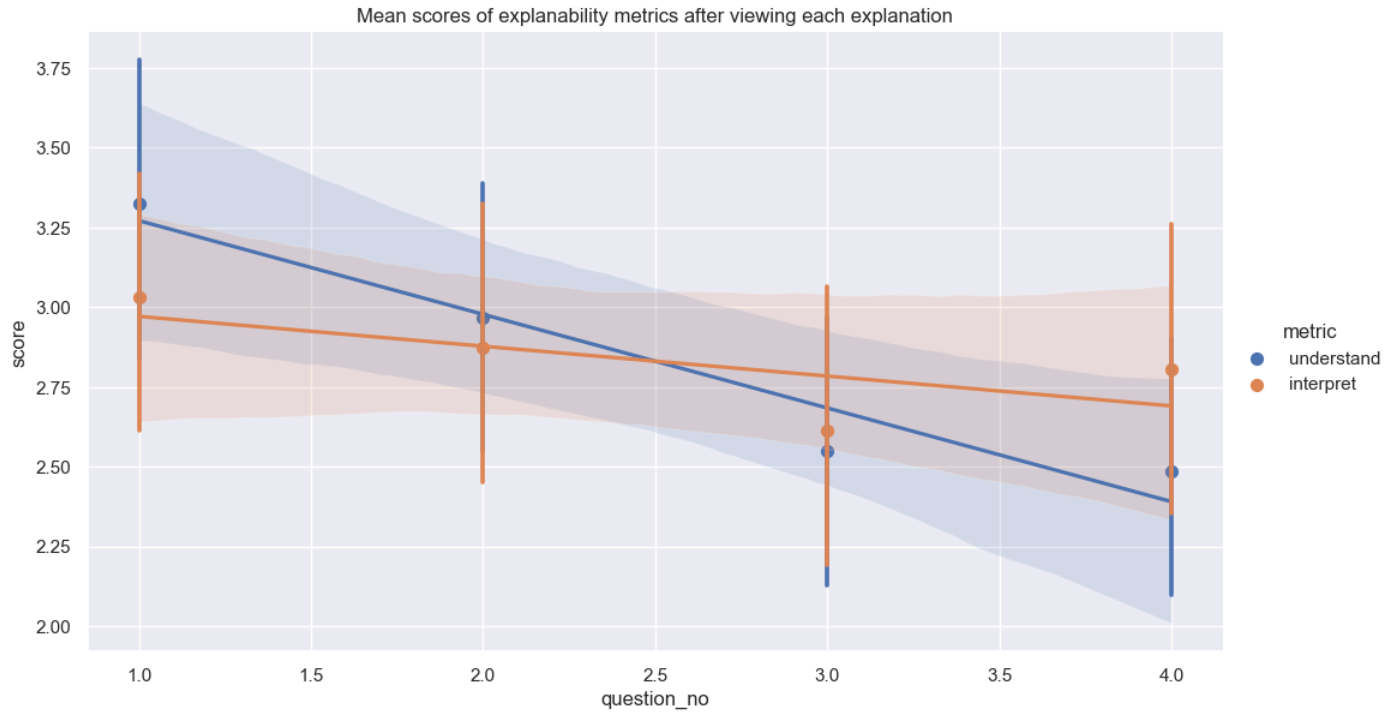
\includegraphics[width=1\linewidth]{figures/part3.png}
  \caption{Trend of the mean of self-reported understanding and interpretability after viewing each explanation}
  \label{fig:part3_trend}
\end{figure}

\begin{figure}[!ht]
  \begin{subfigure}[b]{1\textwidth}
    \centering
    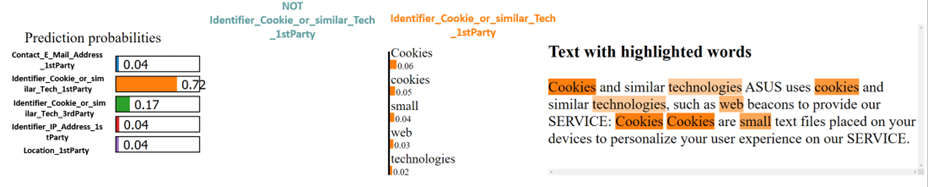
\includegraphics[width=1\linewidth]{figures/explanations_visualisations/section_4a/Picture1.png}
    \caption{1}
  \end{subfigure}
  \hfill
  \begin{subfigure}[b]{1\textwidth}
    \centering
    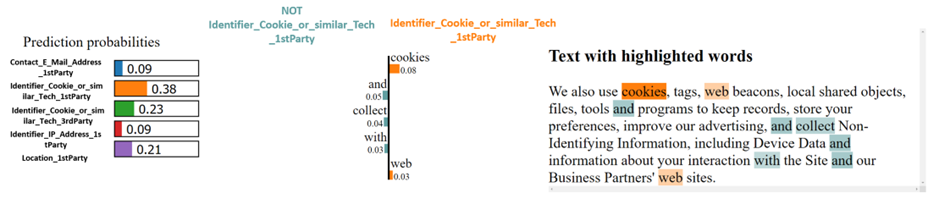
\includegraphics[width=1\linewidth]{figures/explanations_visualisations/section_4a/Picture2.png}
    \caption{2}
  \end{subfigure}
  \hfill
  \begin{subfigure}[b]{1\textwidth}
    \centering
    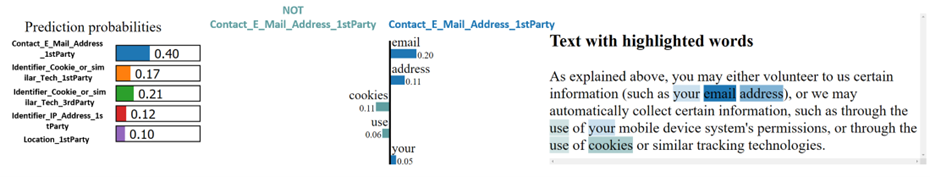
\includegraphics[width=1\linewidth]{figures/explanations_visualisations/section_4a/Picture3.png}
    \caption{3}
  \end{subfigure}
  \hfill
  \begin{subfigure}[b]{1\textwidth}
    \centering
    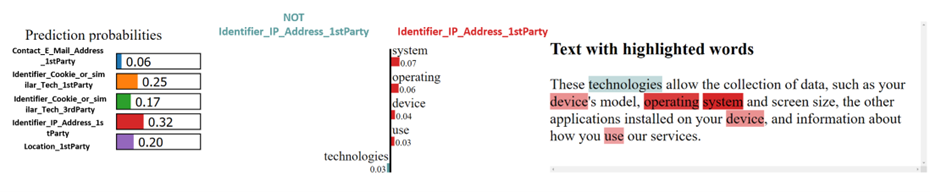
\includegraphics[width=1\linewidth]{figures/explanations_visualisations/section_4a/Picture4.png}
    \caption{4}
  \end{subfigure}
  \caption{The 4 visualisations shown to respondents. Respondents were asked to rate how far they understood why the model made the prediction, and how far they found the visualisation easy to interpret. All 4 sentences were annotated as \texttt{Identifier Cookie 1st Party}.}
  \label{fig:part4_explanations}
\end{figure}

There was a statistically significant decrease in understandability but not interpretability (Table~\ref{tab:p_values_interpret_understand}). Hence, H0 can be rejected in favour of H1. 

A reason for why there was no significant decrease in interpretability was because the questions I posed to the respondents were clear in distinguishing the visualisation from the classifier's logic. Hence, respondents understood how to interpret the visualisation, but were less clear about the classifier's logic that was presented through the visualisation. 

With regards to the significant decrease in understandability, the respondents could be confused about how the model works globally after being exposed to specific predictions that were in themselves explainable, rather than being confused about a specific prediction of the model. As mentioned, the visualisations for this part were specifically chosen to demonstrate the limits of the classifier by changing keywords which were strong predictors of the data practice. This means that respondents were being exposed to a more complex (and confusing) of the model globally as they found contradictions in how the model used certain keywords in some examples but not in others. Therefore, each explanation was actually effective in communicating to the respondents how that particular prediction was made, and therefore could be considered as locally explainable. However, as a whole, respondents' understandability of the model given the contradictions seen through comparing each explanation decreased. Therefore, the classifier could be said to be locally understandable, but globally less understandable.

Another inference is that the underlying explainability method also influences the respondents' perception of the interpretability of the visualisation technique (or vice versa). This can be seen by how there is a positive correlation between the understand and interpret scores. This is not surprising since if the visualisation technique is unclear or poor, understandability of the model itself would also decrease since respondents' only way of viewing the results of the explainability technique is through the visualisation technique. To respondents, both the visualisation technique and the explainability technique are one and the same thing.

\subsection{Analysis of predicting counterfactuals}
Given the lack of any consistent trend of the respondents' votes across the questions (Figure~\ref{fig:part3_counterfactual}), it is difficult to draw any definitive interpretations from the respondents' predictions of counterfactuals. Further, the classifier itself gave ambivalent predicted probabilities for each data practice. For example (Figure~\ref{fig:part3_counterfactual_1}), the classifier predicted \texttt{Contact Email Address} at 25\% while \texttt{Cookie 1st Party} was predicted at 23\%.

\begin{figure}[!ht]
  \begin{subfigure}[b]{1\textwidth}
    \centering
    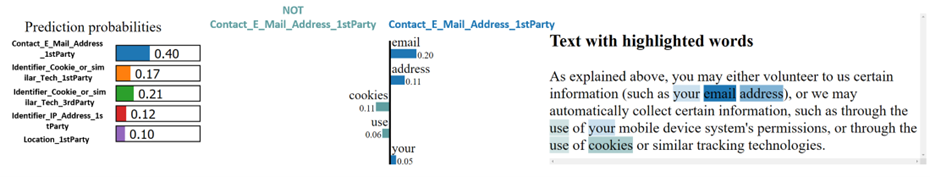
\includegraphics[width=1\linewidth]{figures/explanations_visualisations/counterfactual/3.3.png}
    \caption{Original explanation}
  \end{subfigure}
  \hfill
  \begin{subfigure}[b]{1\textwidth}
    \centering
    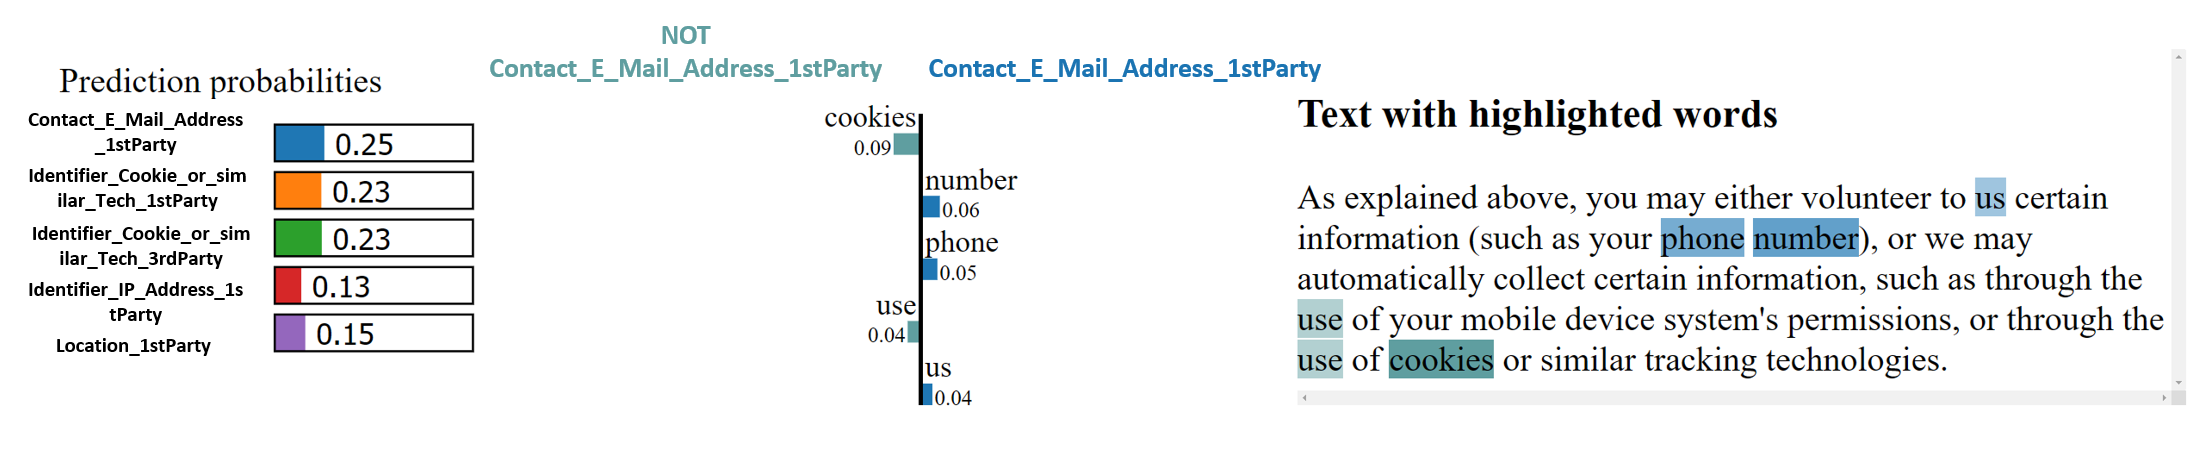
\includegraphics[width=1\linewidth]{figures/explanations_visualisations/counterfactual/3_3_counterfactual.png}
    \caption{Counterfactual explanation (not shown to respondents)}
    \label{fig:part3_counterfactual_1}
  \end{subfigure}
  \caption{Sample counterfactual explanation (1 out of 3)}
  \label{fig:part3_counterfactuals_example}
\end{figure}

\begin{figure}[!ht]
    \centering
    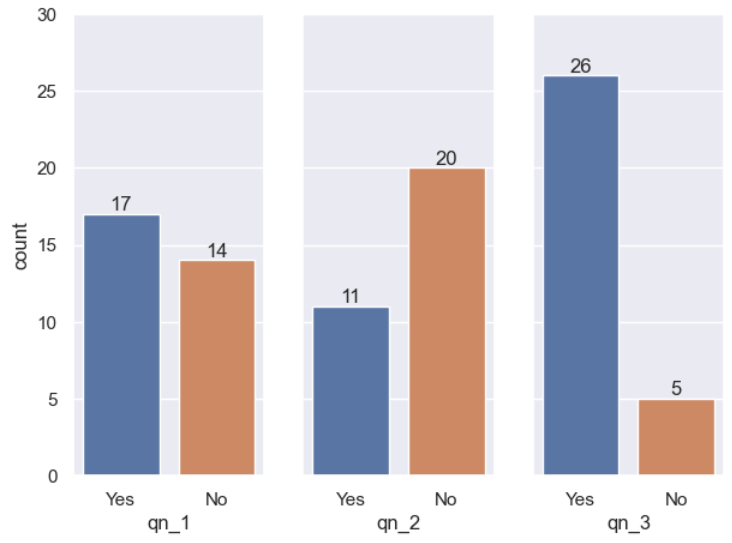
\includegraphics[width=1\linewidth]{figures/part_3_counterfactual.png}
    \caption{Votes for predicting whether counterfactual would be classified as \texttt{Identifier\_Cookie\_1st\_Party}}
    \label{fig:part3_counterfactual}
\end{figure}

\section{Part 4 \& 5: Testing which model and text representation is more explainable}
As there were three questions in each section to test the explainability of each pair of text representation and model, I totalled up the votes for each option for each part and each question (Figure~\ref{fig:part4} and~\ref{fig:part5}).

Overall, respondents found no difference in understandability between logistic regression and SVC (Figure~\ref{fig:part4}), while it was more contentious when comparing text representations, with a third split across the three options (Figure~\ref{fig:part5}). Remember that classifier performance for each pair actually did not differ significantly. In terms of comparing respondents' votes with the "ground truth" metric of model performance, most respondents would be expected to indicate that there were minimal differences between the understandability of the classifiers. This was seen when comparing logistic regression vs SVC but not seen when comparing Tf-IDF and GloVe. While there is no majority consensus for the comparison of text representations, with votes which were almost equally split instead of being heavily weighted in favour of one option show that respondents were more undecided in the understandability of the models. One inference of such results is that while respondents collectively did not give a definitive answer as to the more explainable word representation, there are still possible differences in understandability even when comparing classifiers of relatively similar performance.

\begin{figure}[!ht]
  \centering
    \begin{subfigure}[b]{0.75\textwidth}
      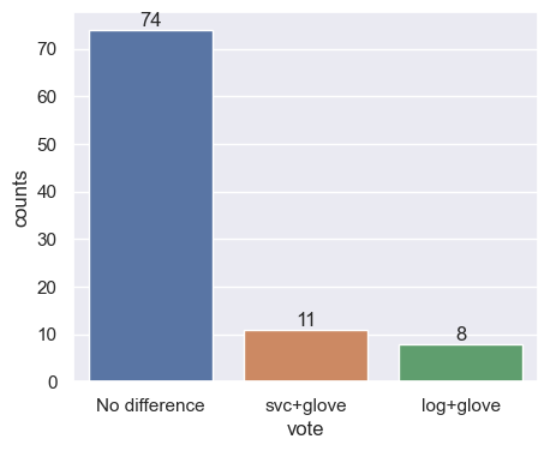
\includegraphics[width=1\linewidth]{figures/part4_votes.png}
      \caption{Total votes across 3 questions}
      %\label{fig:draketl}
    \end{subfigure}
    \hfill
    \centering
    \begin{subfigure}[b]{1\textwidth}
      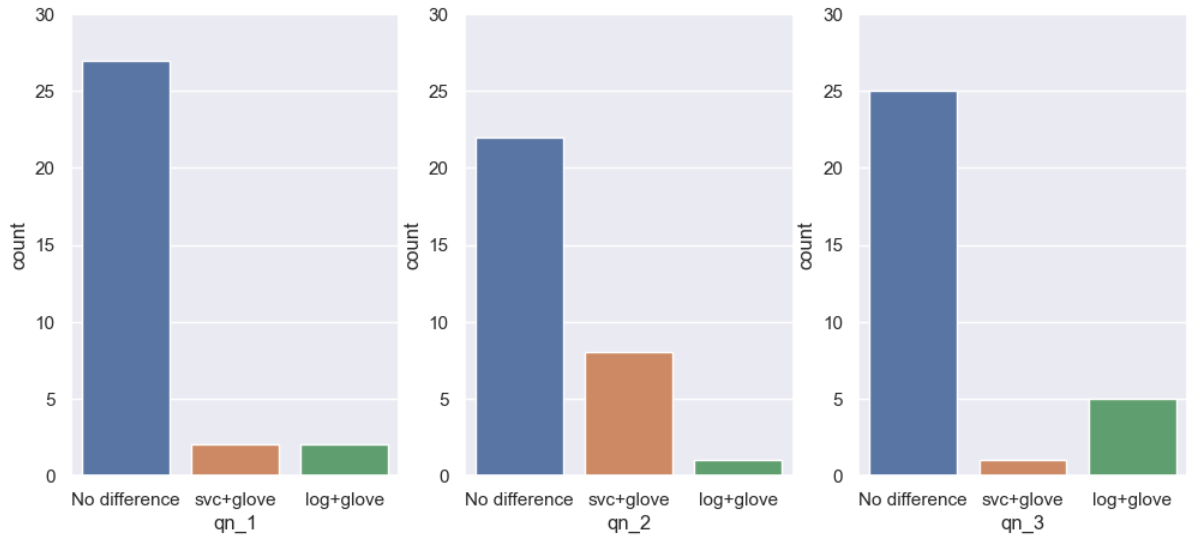
\includegraphics[width=1\linewidth]{figures/part_4_votes_1.png}
      \caption{Votes per question}
    \end{subfigure}
    \caption{Respondents' votes to whether SVC + GloVe or Logistic regression + GloVe were more understandable}
    \label{fig:part4}
\end{figure}

\begin{figure}[!ht]
  \centering
    \begin{subfigure}[b]{0.75\textwidth}
      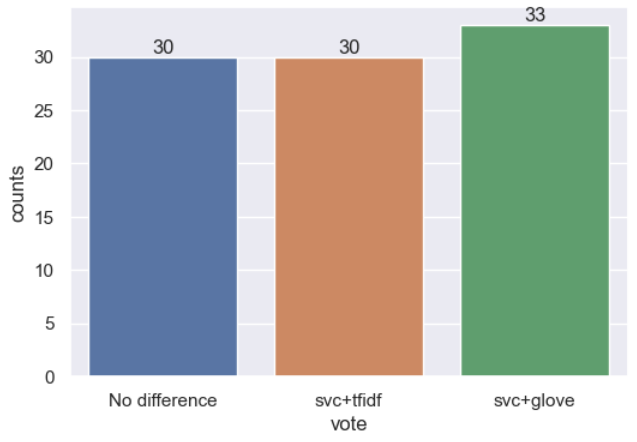
\includegraphics[width=1\linewidth]{figures/part5_votes.png}
      \caption{Total votes across 3 questions}
      %\label{fig:draketl}
    \end{subfigure}
    \hfill
    \centering
    \begin{subfigure}[b]{1\textwidth}
      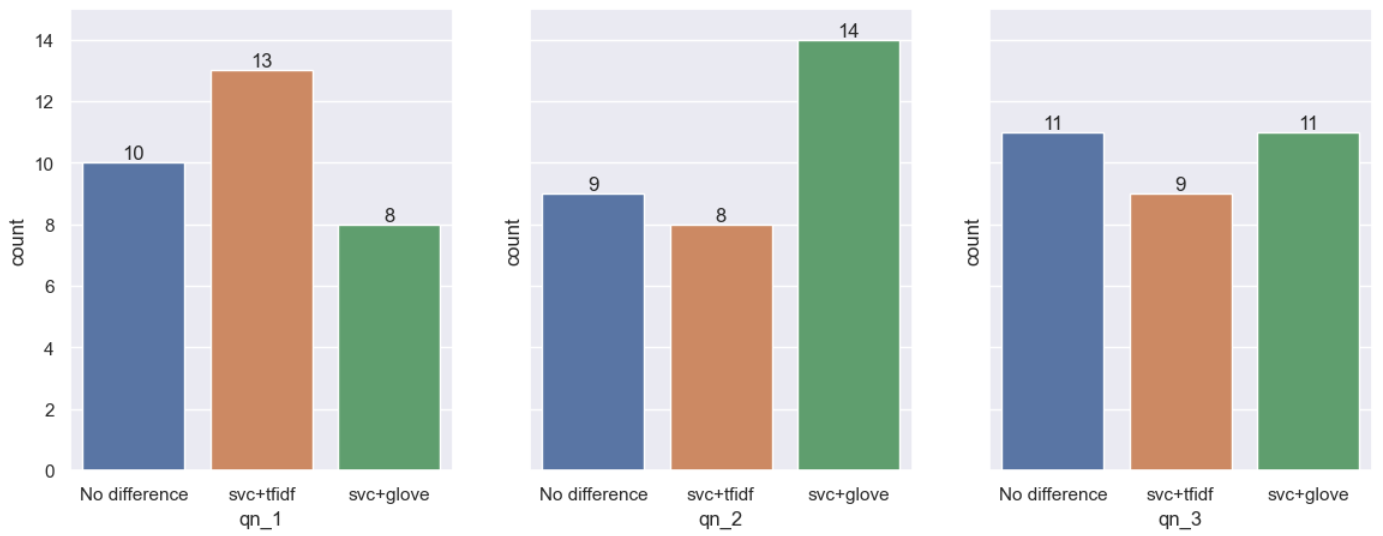
\includegraphics[width=1\linewidth]{figures/part_5_votes_1.png}
      \caption{Votes per question}
    \end{subfigure}
    \caption{Respondents' votes to whether SVC + TfIDF or SVC + GloVe were more understandable}
    \label{fig:part5}
\end{figure}

% Chapter Template
\chapter{Discussion of survey results}

\label{chapter5}

\section{Summary of results}
In total, 31 responses were collected. The table~\ref{tab:demo_1} below show the demographic data and aggregated responses relating to respondents' beliefs regarding AI and data privacy. While I originally intended to conduct analysis of the results across different demographics, there were limited non-law respondents. Therefore, I segmented the analysis that follows according to law (58\%) vs non-law (42\%) respondents.

\begin{table}[!ht]
    \resizebox{\textwidth}{!}{
    \begin{tabular}{|p{0.45\linewidth}|l|l|}
    \hline
    \textbf{Major / Expected major}                    & \textbf{Count} & \textbf{Percentage of total (\%)} \\ \hline
    Law                                                & 18             & 58                                \\ \hline
    MCS / Computer Science / Data Science / Statistics & 3              & 9.7                               \\ \hline
    Psychology                                         & 3              & 9.7                               \\ \hline
    Global Affairs / Political Science                 & 2              & 6.5                               \\ \hline
    Environmental Studies                              & 1              & 3.2                               \\ \hline
    Economics                                          & 1              & 3.2                               \\ \hline
    Life Sciences                                      & 1              & 3.2                               \\ \hline
    Philosophy                                         & 1              & 3.2                               \\ \hline
    Policy                                             & 1              & 3.2                               \\ \hline
    \end{tabular}
    }
    \caption{Demographic breakdown of respondents according to academic discipline}
    \label{tab:demo_1}
\end{table}

\subsection{Part 1: Beliefs relating to AI \& data privacy}
Except for the questions relating to subject matter expertise (data privacy and AI), the level of agreement of law vs non-law respondents were about the same (Figure~\ref{fig:demo_3}). Law respondents had less expertise in AI, while conversely, non-law respondents had less experience with data privacy. Across all respondents, while they rated that decisions by AI could be a risk to society (about 4), they also agreed that decisions by AI could be equally useful. This suggests that the respondents think the balance between "usefulness" and "risks" are not zero-sum; AI could be very helpful in solving problems, but at the same time users should be cognisant of the risks. Such a view seems optimistic, but also realistic.

\begin{figure}[!ht]
    \begin{subfigure}[b]{1\textwidth}
      \centering
      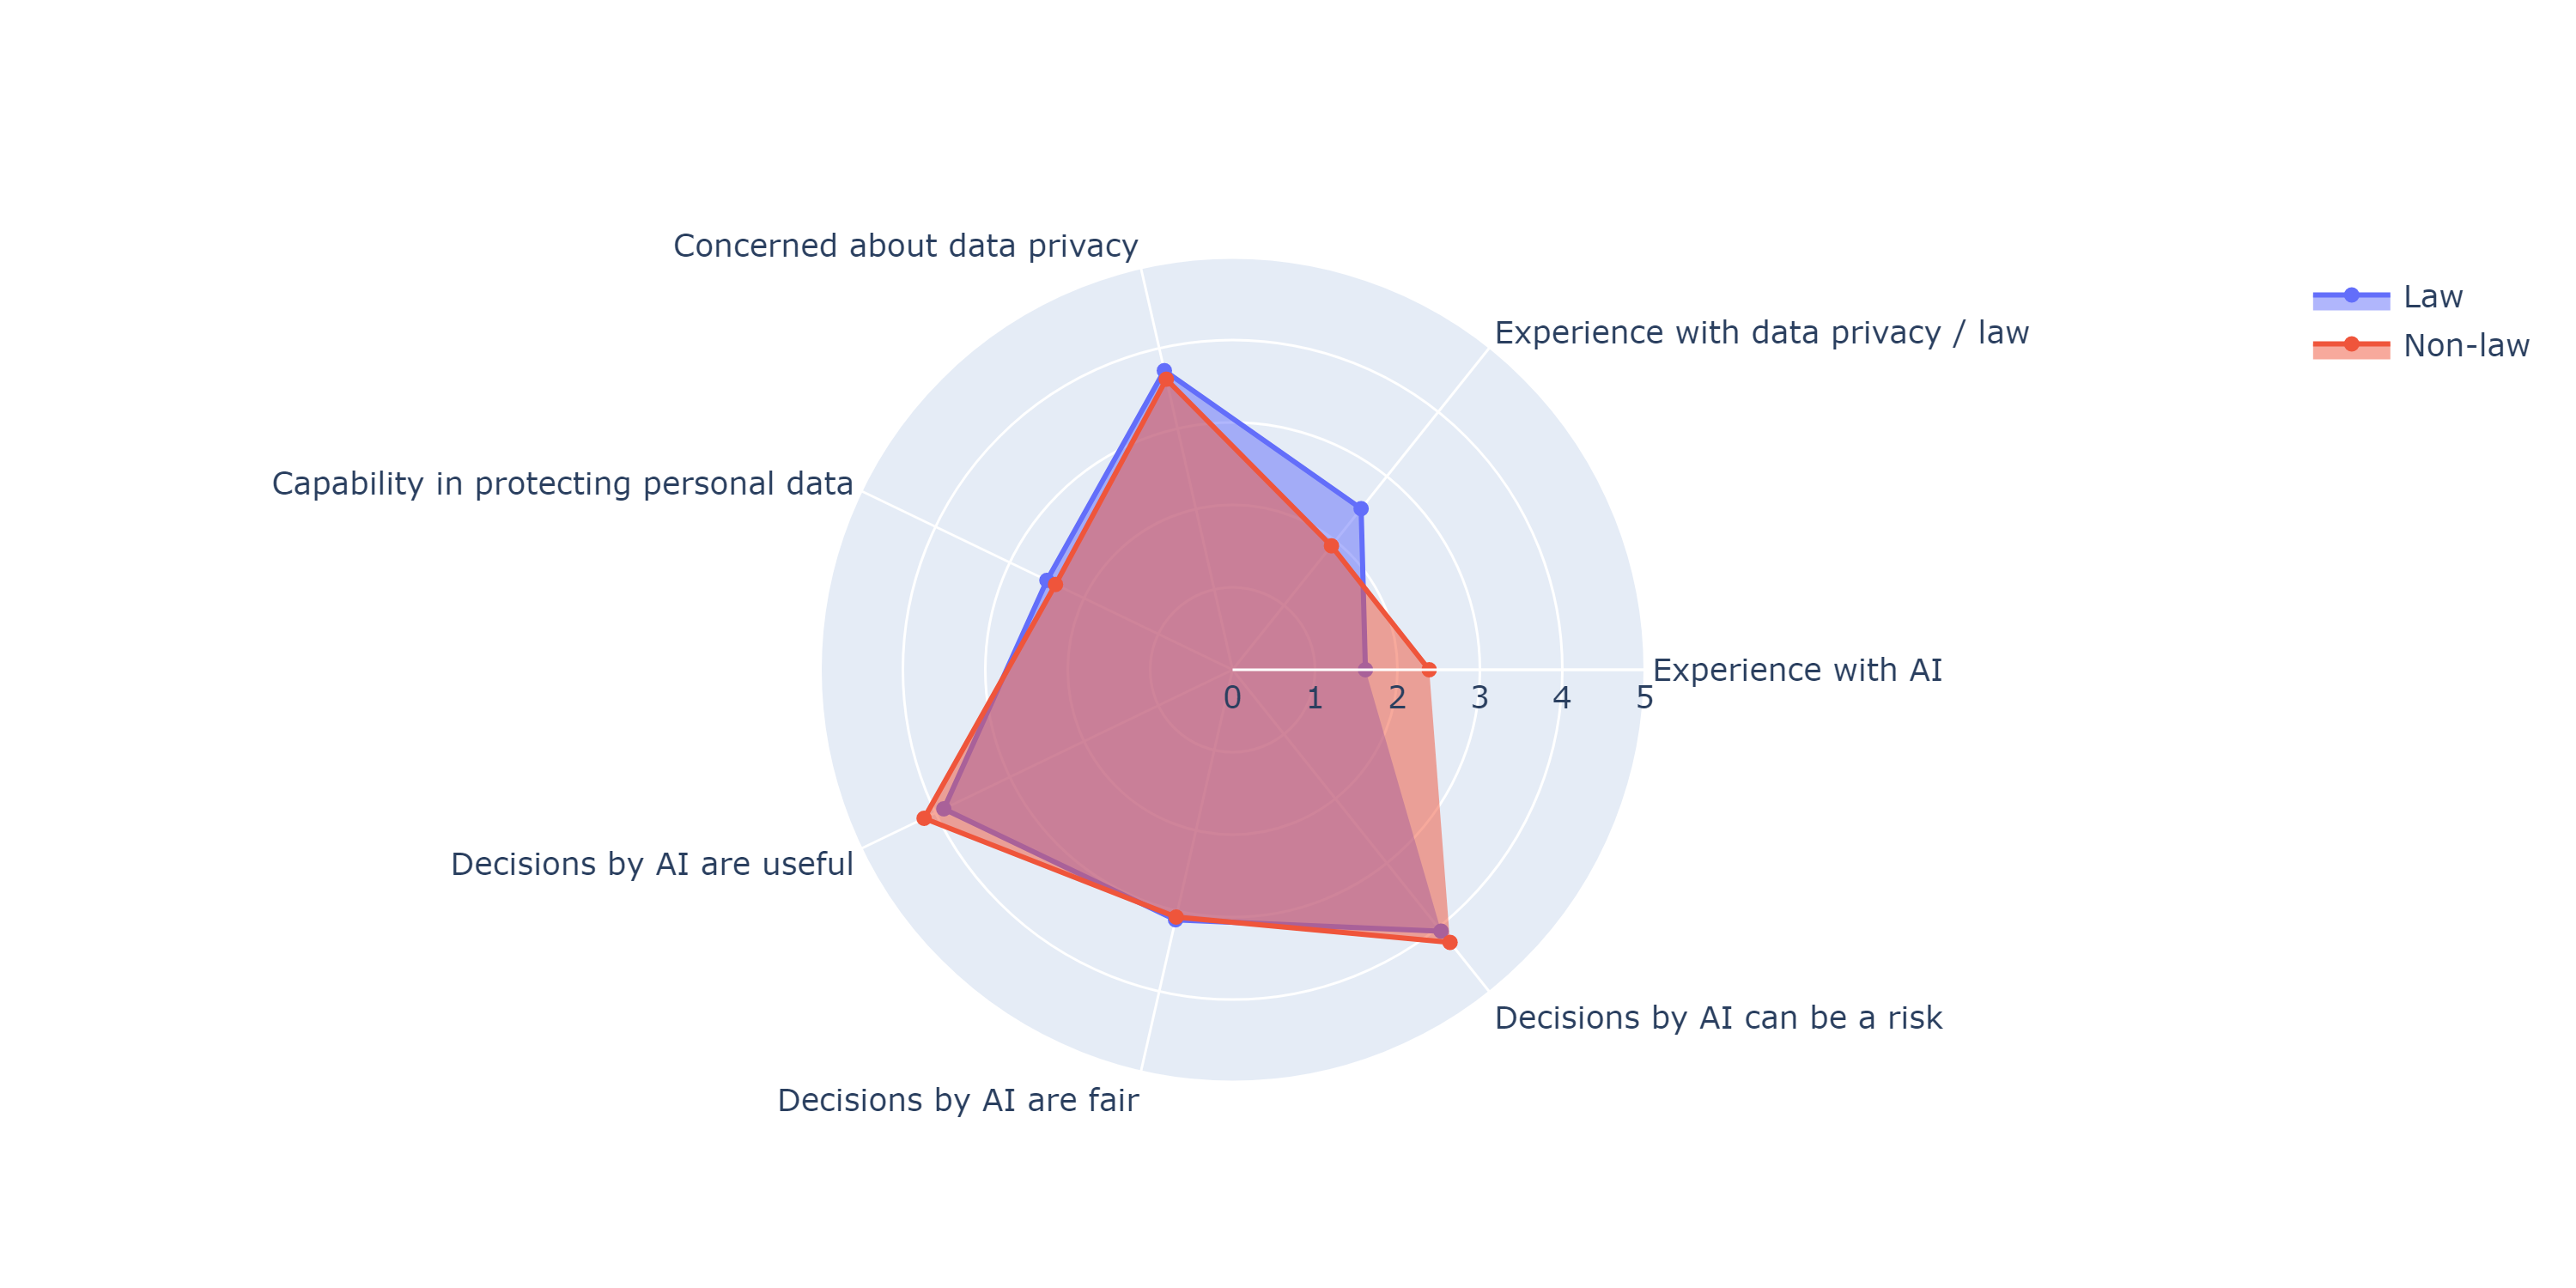
\includegraphics[width=1\linewidth]{figures/demo_3.png}
      \caption{Law vs Non-law respondents}
      %\label{fig:draketl}
    \end{subfigure}
    \hfill
    \begin{subfigure}[b]{1\textwidth}
      \centering
      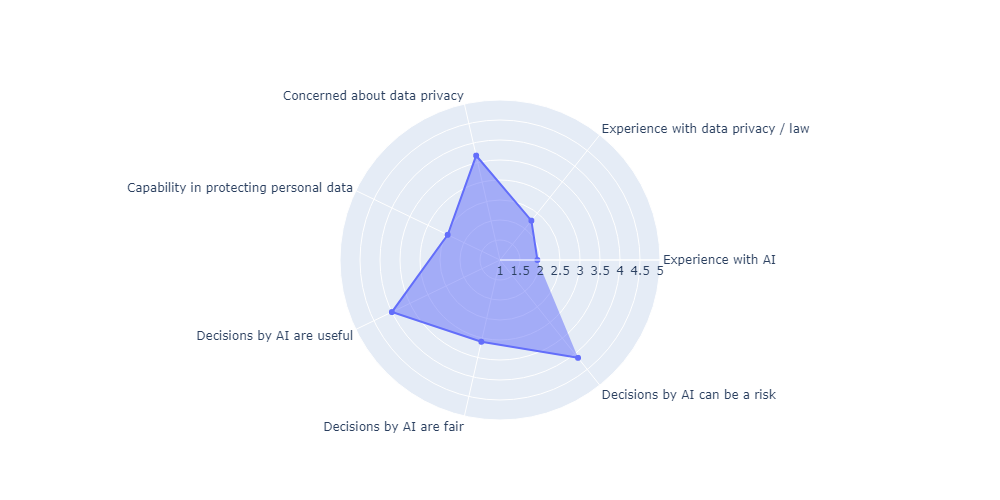
\includegraphics[width=1\linewidth]{figures/demo_4.png}
      \caption{All respondents}
    \end{subfigure}
    \caption{Mean scores of self-reported beliefs of respondents regarding AI \& data privacy. (1 = least agree, 5 = strongly agree. $n=31$)}
    \label{fig:demo_3}
\end{figure}

\subsection{Part 2 \& Part 6: Comparison of self-reported scores of explainability across the three contexts}
Using the Wilcoxon Rank Sum Test, I tested for the following, setting $\alpha = 0.1$: 
\begin{align*}
    H0&: \text{There is no increase / decrease in scores after viewing the explainations.} \\
    H1&: \text{There is an increase / decrease in scores after viewing the explainations.}
\end{align*}

The 1-sided test was used to check whether the distribution underlying the difference between the initial and final paired scores was symmetric below or above 0 (\cite{scipy}). Mathematically it can be stated as $d = i - f$, where $i$ and $f$ are the scores reported before and after viewing the explanations, and $d$ is the difference. Hence, if $d < 0$, then $i < f$ and the scores increased after viewing, and $d > 0$, then $i > f$ and the scores decreased after viewing.

\begin{table}[!ht]
    \centering
    \resizebox{\textwidth}{!}{    
    \begin{tabular}{|p{0.3\textwidth}|p{0.15\textwidth}|p{0.15\textwidth}|p{0.15\textwidth}|p{0.15\textwidth}|p{0.15\textwidth}|p{0.15\textwidth}|}
    \hline
        \textbf{Question} & \textbf{Context 1: Increase} & \textbf{Context 1: Decrease} & \textbf{Context 2: Increase} & \textbf{Context 2: Decrease} & \textbf{Context 3: Increase} & \textbf{Context 3: Decrease} \\ \hline
        \textbf{Do you think model is effective?} & \cellcolor{red!25}0.013 & 0.987 & 0.932 & \cellcolor{red!25}0.0684 & 0.856 & 0.144 \\ \hline
        \textbf{Do you think model is a fair method?} & 0.382 & 0.618 & 0.841 & 0.159 & 0.933 & \cellcolor{red!25}0.0671 \\ \hline
        \textbf{Do you think model is a risk to society?} & 0.756 & 0.244 & 0.428 & 0.572 & 0.825 & 0.175 \\ \hline
        \textbf{Do you trust the prediction of the model?} & 0.887 & 0.113 & 0.945 & \cellcolor{red!25}0.055 & 0.837 & 0.163 \\ \hline
    \end{tabular}
    }
    \caption{p-values comparing whether there was a statistically significant increase / decrease in the explainability scores before and after viewing explanations.}
    \label{tab:context_comparison}
\end{table}

\begin{table}[!ht]
    \centering
    \begin{subtable}{0.5\textwidth}
        \begin{tabular}{|l|l|}
        \hline
            \textbf{Context} & \textbf{p-value} \\ \hline
            1: Increase & 0.369 \\ \hline
            1: Decrease & 0.633 \\ \hline
            2: Increase & 0.940 \\ \hline
            2: Decrease & \cellcolor{red!25}0.060 \\ \hline
            3: Increase & 0.955 \\ \hline
            3: Decrease & \cellcolor{red!25}0.0450 \\ \hline
        \end{tabular}
        \caption{p-values averaged across metrics, compared by contexts}
        \label{tab:context_comparison_2a}
    \end{subtable}
    \hfill
    \begin{subtable}{0.5\textwidth}
        \begin{tabular}{|l|l|}
            \textbf{Metric}                                    & \textbf{p-value}                     \\ \hline
            Effective: Increase & 0.485  \\ \hline
            Effective: Decrease & 0.515  \\ \hline
            Fair: Increase      & 0.826  \\ \hline
            Fair: Decrease      & 0.174  \\ \hline
            Risk: Increase      & 0.660  \\ \hline
            Risk : Decrease     & 0.340  \\ \hline
            Trust: Increase     & 0.953  \\ \hline
            Trust: Decrease     & \cellcolor{red!25}0.0468 \\ \hline
        \end{tabular}
        \caption{p-values averaged across contexts, compared by metrics}
        \label{tab:context_comparison_2b}
    \end{subtable}
    \caption{p-values comparing aggregated scores by context and metric}
    \label{tab:context_comparison_2}
\end{table}

\begin{table}[!ht]
    \centering
    \begin{tabular}{|l|l|}
        \hline
        \textbf{Increase} & \textbf{Decrease} \\ \hline
        0.844             & 0.156           \\ \hline
    \end{tabular}
    \caption{p-values comparing aggregated scores across contexts and metrics}
    \label{tab:context_comparison_3}
\end{table}

The p-values are reported in Table~\ref{tab:context_comparison} ,~\ref{tab:context_comparison_2} and~\ref{tab:context_comparison_3}. "Increase" and "decrease" refer to the p-values of the test to check whether the scores significantly increased or decreased. Here are the instances when $p<0.1$, and therefore $H0$ can be rejected in favour of $H1$ such that there was a significant increase / decrease of scores after viewing the explanations:
\begin{enumerate}
    \item There is a statistically significant decrease in explainability for context 1 and 2 when aggregating across the metrics (Table~\ref{tab:context_comparison_2a}) and for trust when aggregating across the three contexts (Table~\ref{tab:context_comparison_2b}).
    \item In particular, effectiveness and trust significantly decreased for context 2, and fairness significantly decreased for context 3 (Table~\ref{tab:context_comparison}). 
    The overall explainability aggregated across both contexts and metrics did not significantly increase / decrease (Table~\ref{tab:context_comparison_3}).
\end{enumerate}

Here are some inferences that could be drawn from these observations:
\begin{enumerate}
    \item 
\end{enumerate}

\subsection{Part 3: Testing whether viewing more visualisations increase explainability}
From Figure~\ref{fig:part3_trend}, a decreasing trend of both understand and interpret after viewing each explanation, though understanding has a more negative gradient than interpret. Keeping in mind that the question asked was whether the respondent found the model's prediction more understandable and whether the visualisation was easier to interpret, respondents found the model less generally explainable after viewing more explanations, both in terms of the method of visualising the explanation, as well as understanding the inner logic of the model. 

A direct interpretation of this decreasing trend suggests that the model and LIME were not very effective. However, this could also be interpreted as the respondents being more confused about how the model works globally after being exposed to more nuanced details about the model, rather than being confused about a specific prediction of the model. As mentioned in Chapter~\ref{chapter2}, the visualisations for this part were specifically chosen to demonstrate the limits of the model by changing keywords which were strong predictors of the data practice. This means that respondents were getting a more complex (and confusing) conception of the model globally as they found contradictions in how the model used certain keywords in some examples but not in others. Therefore, each explanation was actually effective in communicating to the respondents how that particular prediction was made, but as a whole how the model functioned was not understandable given the contradictions between each explanation. This decrease in explainability could be likened to a variation of the Dunning-Kruger effect (\cite{dunning_kruger}), whereby the respondents who initially had no experience with the model believed that they understood the model well because they were unaware of the complexity of the model, but when they were given more information, they had more awareness of the complexity and therefore reported a drop in explainability of the model as a whole.

\begin{figure}[!ht]
    \centering
    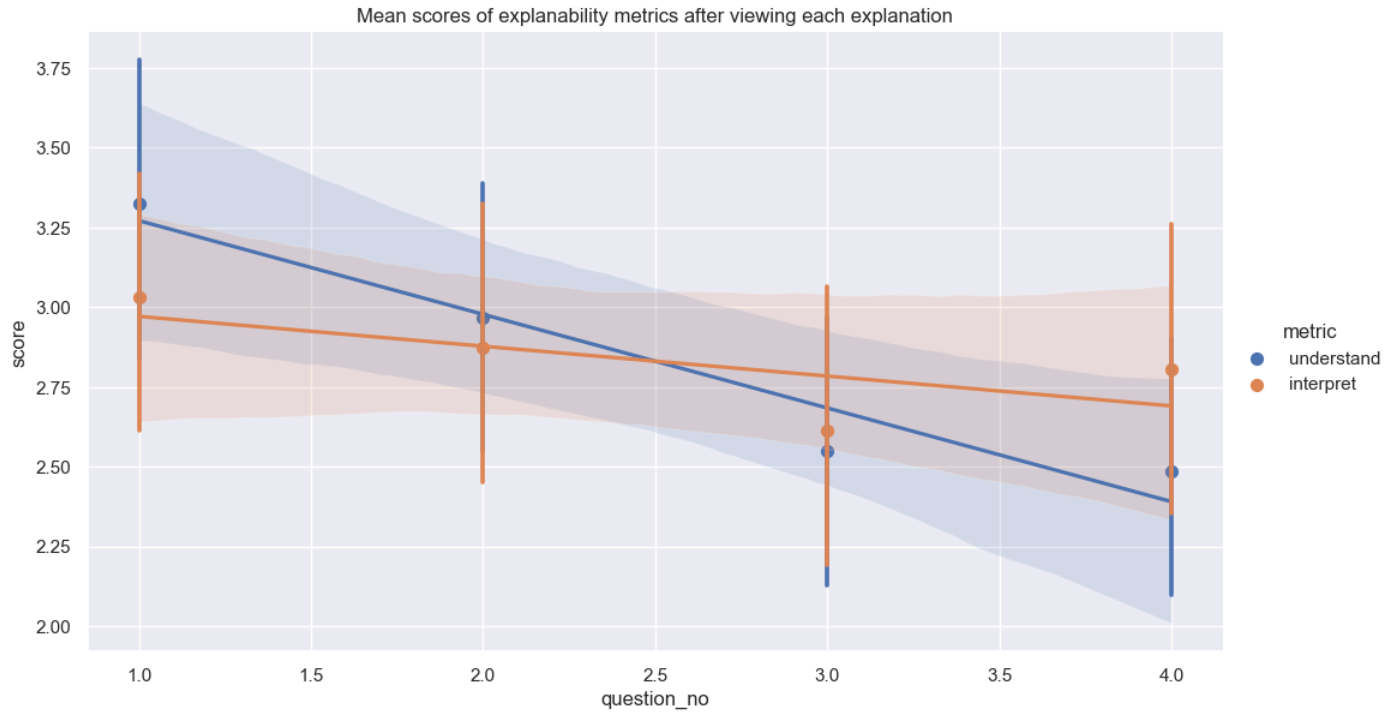
\includegraphics[width=1\linewidth]{figures/part3.png}
    \caption{Trend of the mean of self-reported understanding and interpretability after viewing each explanation}
    \label{fig:part3_trend}
\end{figure}

(need to add the visualisations for the counterfactuals here)

Since the model itself gave quite ambivalent predicted probabilities for each data practice, the respondents' votes of predicting whether these counterfactuals would be classified as \texttt{Identifier\_Cookie} should also be equally ambivalent if the respondents actually had a good sense of how the model would predict. Only the results of the first question had some similarity to the predicted probabilities of the model, while the results of the third question differed the most from the model. Nevertheless, given the lack of any consistent trend across the questions, it is difficult to draw any definitive interpretations from this section.

\begin{figure}[!ht]
    \centering
    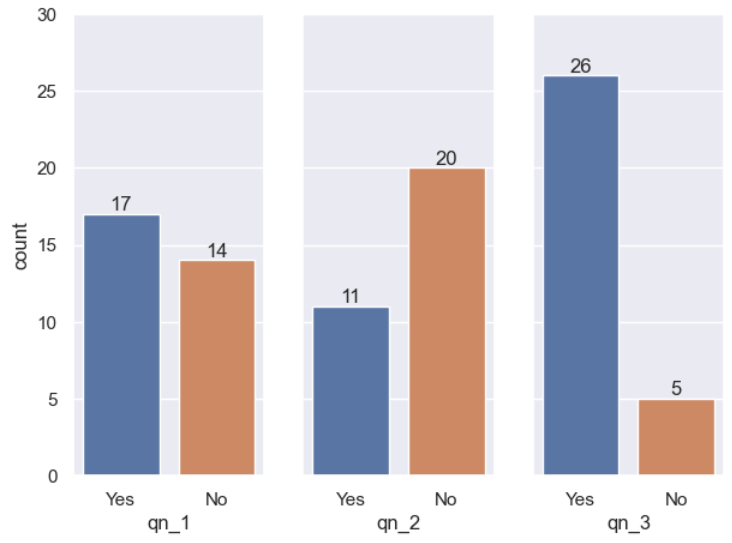
\includegraphics[width=1\linewidth]{figures/part_3_counterfactual.png}
    \caption{Votes for predicting whether counterfactual would be classified as \texttt{Identifier\_Cookie\_or\_Similar\_Tech\_1st\_Party}}
    \label{fig:part3_counterfactual}
\end{figure}

\subsection{Part 4 \& 5: Testing which model and word representation is more explainable}
Overall, respondents found no difference between logistic regression and SVC (Figure~\ref{fig:part4}), while it was more contentious for the word representation, with a third split across the three categories (Figure~\ref{fig:part5}). For logistic regression vs SVC, the results coincided with the performance of the classifiers. However for word representations , I found GloVE more explainable than Tf-IDF. While there is no majority consensus in favour of GloVe, the fact that the votes were almost equally split instead of being heavily weighted in favour of one category shows that respondents were more undecided. This means that while respondents might not be able to accurately discern which was the more explainable word representation as compared to an expert in the field, they still have some level of intuition when there are differences in the components of the models used. This suggests that LIME used in this context has a decent level of explainability, if not the distribution of votes for Part 4 \& Part 5 would be roughly equivalent.

\begin{figure}[!ht]
    \begin{subfigure}[b]{0.75\textwidth}
      \centering
      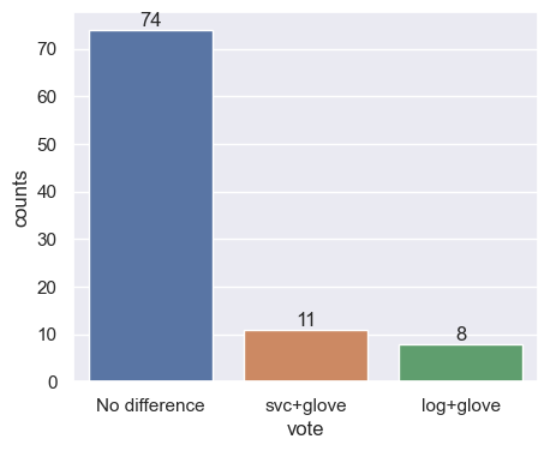
\includegraphics[width=1\linewidth]{figures/part4_votes.png}
      \caption{Total votes across 3 questions}
      %\label{fig:draketl}
    \end{subfigure}
    \hfill
    \begin{subfigure}[b]{1\textwidth}
      \centering
      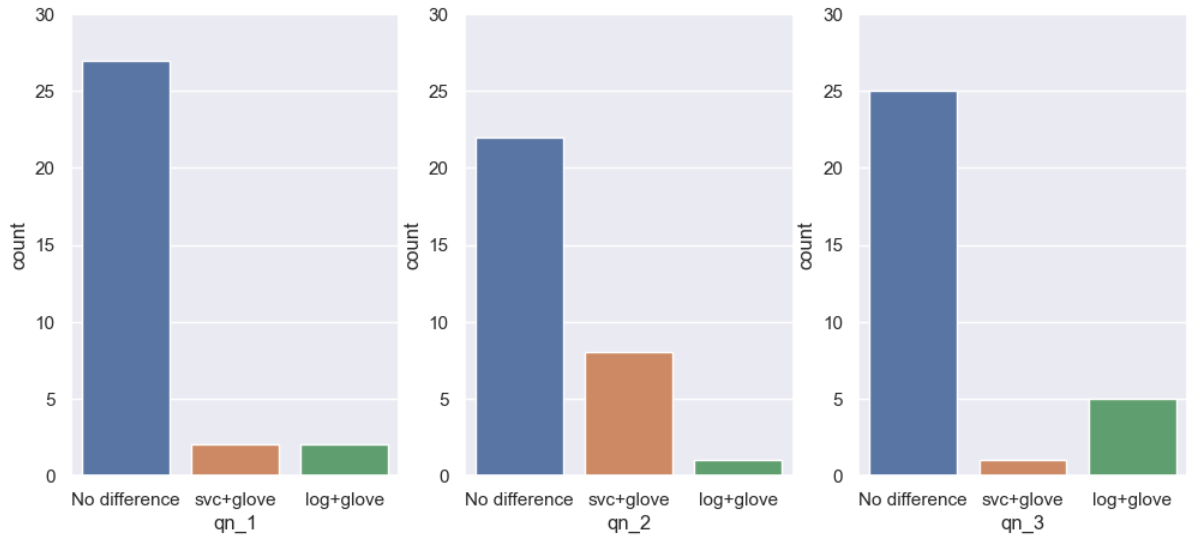
\includegraphics[width=1\linewidth]{figures/part_4_votes_1.png}
      \caption{Votes per question}
    \end{subfigure}
    \caption{Testing for which model was more explainable: Respondents' votes to whether SVC + GloVe or Logistic regression + GloVe were more explaninable}
    \label{fig:part4}
\end{figure}

\begin{figure}[!ht]
    \begin{subfigure}[b]{0.75\textwidth}
      \centering
      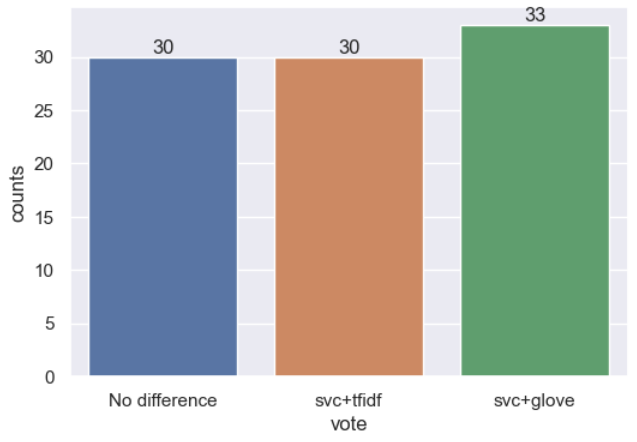
\includegraphics[width=1\linewidth]{figures/part5_votes.png}
      \caption{Total votes across 3 questions}
      %\label{fig:draketl}
    \end{subfigure}
    \hfill
    \begin{subfigure}[b]{1\textwidth}
      \centering
      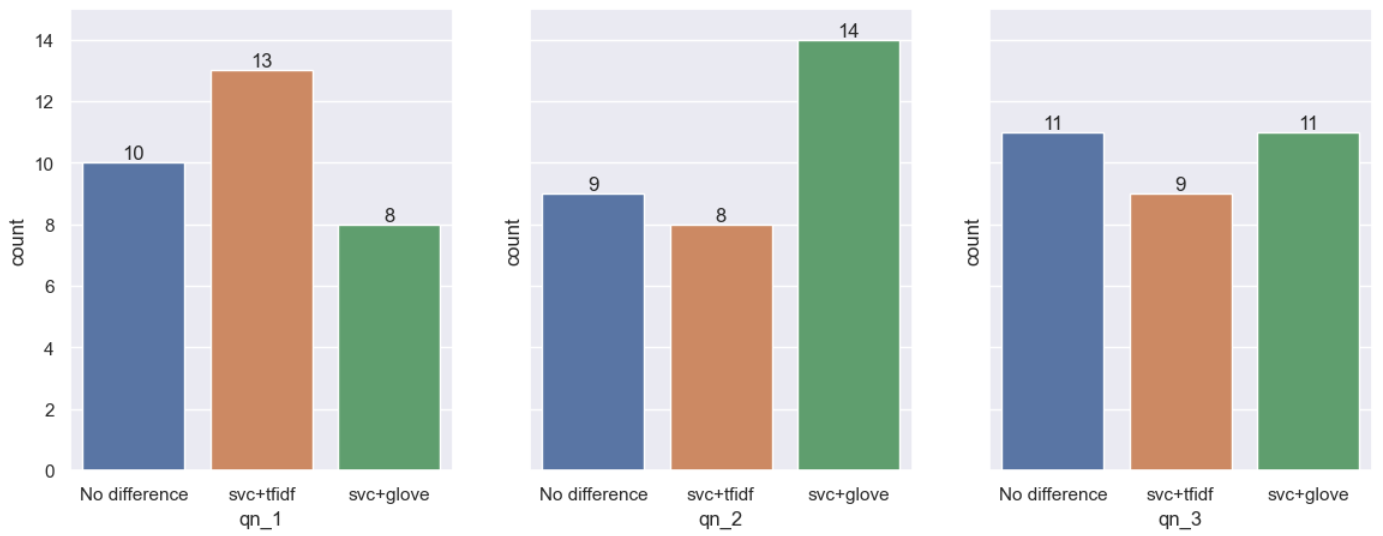
\includegraphics[width=1\linewidth]{figures/part_5_votes_1.png}
      \caption{Votes per question}
    \end{subfigure}
    \caption{Testing for which word representation was more explainable: Respondents' votes to whether SVC + TfIDF or SVC + GloVe were more explaninable}
    \label{fig:part5}
\end{figure}

\subsection{General interpretation of results}


%----------------------------------------------------------------------------------------
%	BIBLIOGRAPHY
%----------------------------------------------------------------------------------------

\printbibliography[heading=bibintoc]

%----------------------------------------------------------------------------------------
%	THESIS CONTENT - APPENDICES
%----------------------------------------------------------------------------------------

\appendix % Cue to tell LaTeX that the following "chapters" are Appendices

% Include the appendices of the thesis as separate files from the Appendices folder
% Uncomment the lines as you write the Appendices

 % Appendix A

\chapter{Survey Questions} % Main appendix title

\label{AppendixA} % For referencing this appendix elsewhere, use \ref{AppendixA}

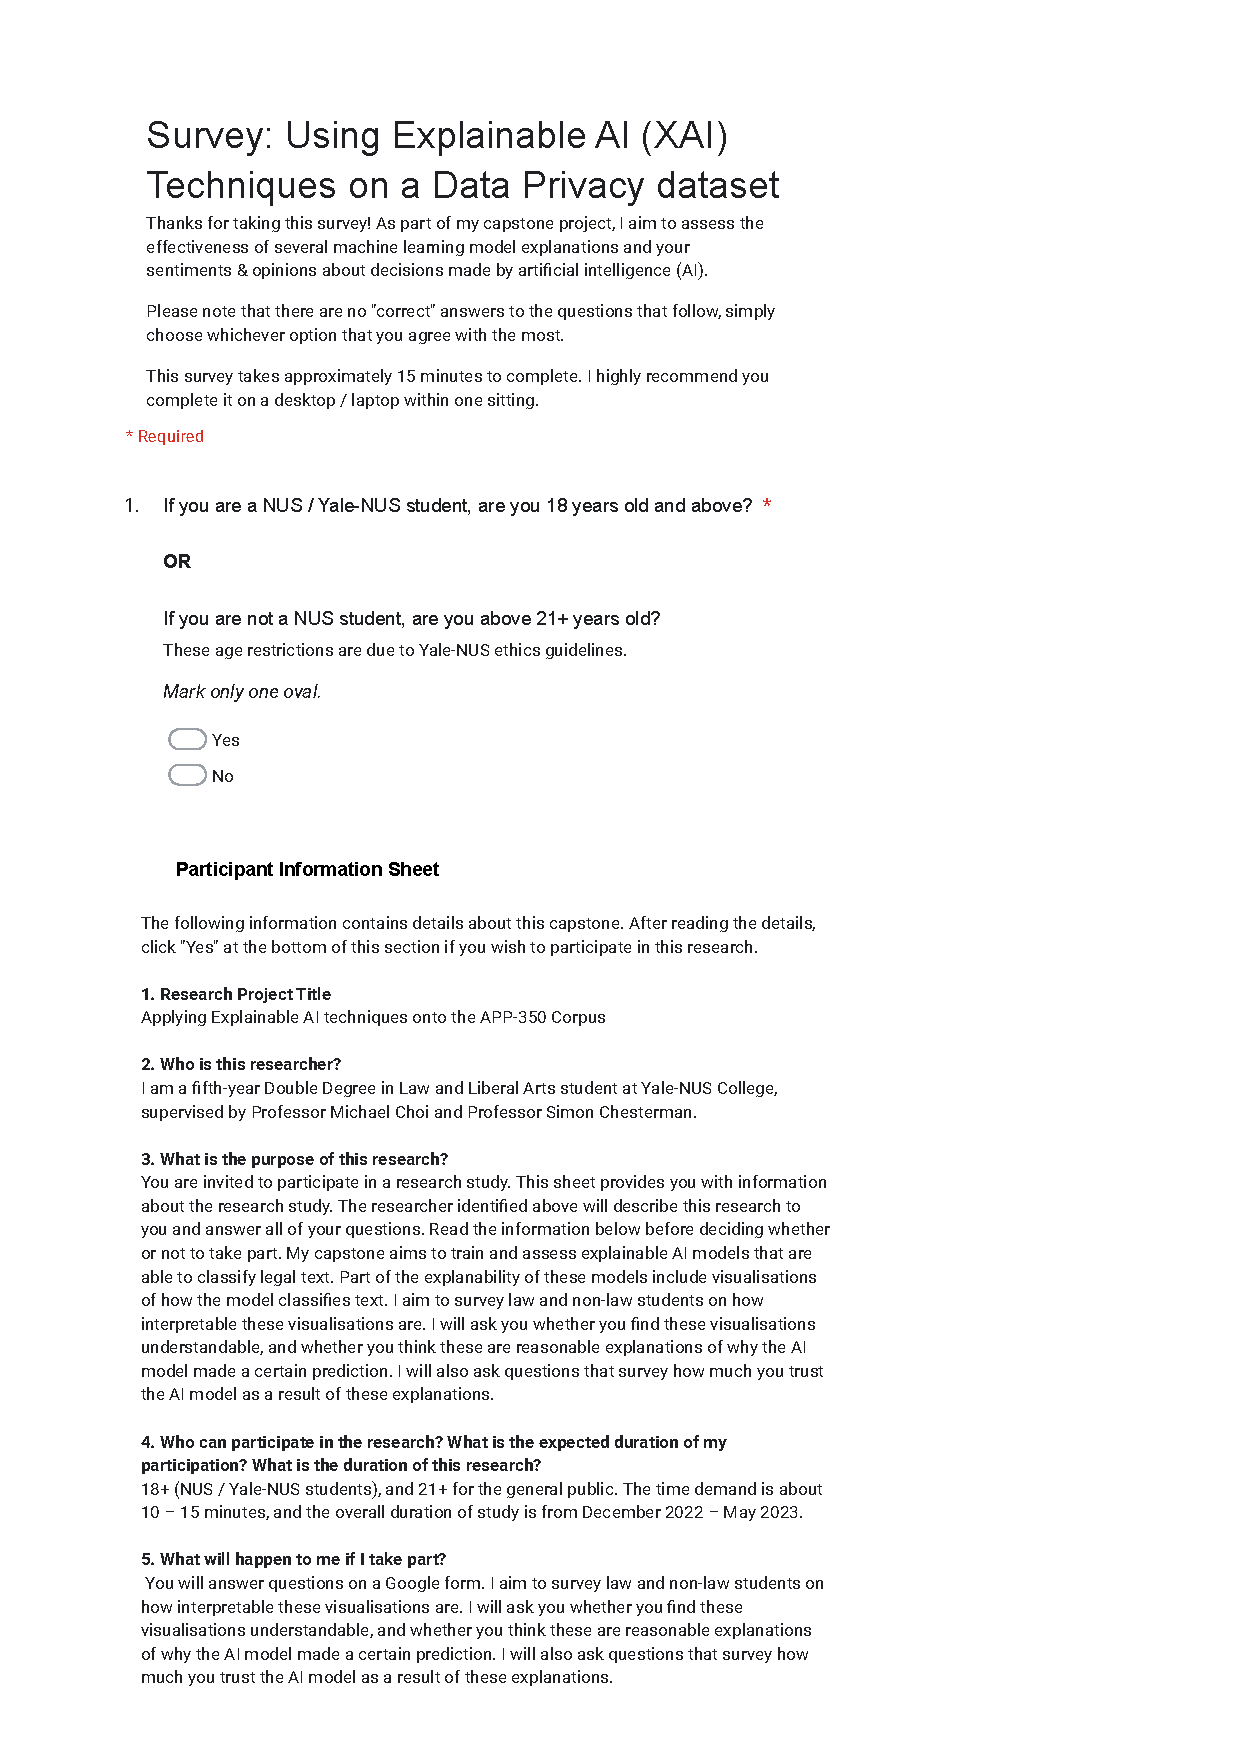
\includepdf[pages=-, pagecommand={},width=\textwidth]{../appendix/survey_questions.pdf}

% \noindent If you want to have obvious links in the PDF but not the printed text, use:

% {\small\verb!\hypersetup{colorlinks=false}!}.


%----------------------------------------------------------------------------------------

\end{document}
